% defer/rcu.tex
% mainfile: ../perfbook.tex
% SPDX-License-Identifier: CC-BY-SA-3.0

\section{Read-Copy Update (RCU)}
\label{sec:defer:Read-Copy Update (RCU)}
%
\epigraph{``Free'' is a \emph{very} good price!}{Tom Peterson}

All of the mechanisms discussed in the preceding sections
used one of a number of approaches to defer specific actions
until they may be carried out safely.
The reference counters discussed in
\cref{sec:defer:Reference Counting}
use explicit counters to defer actions that could disturb readers,
which results in read-side contention and thus poor scalability.
The hazard pointers covered by
\cref{sec:defer:Hazard Pointers}
use implicit reference counters in the guise of per-thread lists of
pointers.
This avoids read-side contention, but requires readers to do stores and
conditional branches, as well as either \IXhpl{full}{memory barrier}
in read-side primitives or real-time-unfriendly \IXacrlpl{ipi} in
update-side primitives.\footnote{
	In some important special cases, this extra work can be avoided
	by using link counting as exemplified by the UnboundedQueue
	and ConcurrentHashMap data structures implemented in Folly
	open-source library
	(\url{https://github.com/facebook/folly}).}
The sequence lock presented in
\cref{sec:defer:Sequence Locks}
also avoids read-side contention, but does not protect pointer
traversals and, like hazard pointers, requires either full memory barriers
in read-side primitives, or inter-processor interrupts in update-side
primitives.
These schemes' shortcomings raise the question of
whether it is possible to do better.

This section introduces \IXBacrfst{rcu}, which provides
an API that allows readers to be associated with regions in the source code,
rather than with expensive updates to frequently updated shared data.

Although RCU has gained a reputation for being subtle and difficult,
when used properly, it is quite straightforward.
In fact, no less an authority than Butler Lampson classifies it as easy
concurrency~\cite{ButlerLampson2022ProgrammingConcurrentSystems}.
And Lampson is quite right:
The core concept behind RCU is nothing more than updaters waiting for
all pre-existing readers to complete, but neither blocking nor necessarily
being blocked by new readers.
For their part, Balmau, Guerraoui, Herlihy, and Zablotchi state
``QSBR [a particular class of RCU implementations] is fast and can be
applied to virtually any data structure''.

\QuickQuiz{
	There is no way RCU can be this simple!!!
	What on earth could you \emph{possibly} do with a synchronization
	primitive that is nothing more than a simple delay???
}\QuickQuizAnswer{
	I am sorry, but RCU's core concept really is that simple!
	And you can do many amazing things with RCU's simple delay
	by combining it with combinations of other cleverly chosen
	techniques.
	Please continue reading this section in order to learn how.
}\QuickQuizEnd

On the other hand, making good use of RCU often requires that you think
differently about concurrency in general and about your use case in
particular.
Much of the remainder of this section therefore provides a guide to
mapping use cases onto RCU.

\QuickQuiz{
	Enough of this noise!!!
	Isn't RCU nothing more nor less than a replacement for some
	reader-writer-locking use cases???
}\QuickQuizAnswer{
	It is true that Linux-kernel RCU has been most frequently used
	to replace reader-writer locking on linked data structures.
	In fact, such replacement accounts for about 95\pct\ of the uses
	of RCU in the Linux kernel.
	However,
	\cref{sec:defer:RCU Usage}
	presents many additional (although much less common) RCU use
	cases.
}\QuickQuizEnd

The remainder of this
section examines RCU from a number of different perspectives.
\Cref{sec:defer:Introduction to RCU} provides the classic
introduction to RCU,
\cref{sec:defer:RCU Fundamentals} covers fundamental RCU
concepts,
\cref{sec:defer:RCU Linux-Kernel API} presents the Linux-kernel
API,
\cref{sec:defer:RCU Usage} introduces some common RCU use cases,
and finally
\cref{sec:defer:RCU Related Work} covers recent work related
to RCU.

% defer/rcuintro.tex
% mainfile: ../perfbook.tex
% SPDX-License-Identifier: CC-BY-SA-3.0

\subsection{Introduction to RCU}
\label{sec:defer:Introduction to RCU}

The approaches discussed in the preceding sections have provided
good scalability but decidedly non-ideal performance for the
Pre-BSD routing table.
Therefore, in the spirit of ``only those who have gone too far
know how far you can go'',\footnote{
	With apologies to T.~S.~Eliot.}
we will go all the way, looking into algorithms in which concurrent
readers might well execute exactly the same sequence of assembly language
instructions as would a single-threaded lookup, despite the presence of
concurrent updates.
Of course, this laudable goal might raise serious implementability
questions, but we cannot possibly succeed if we don't even try!

And should we succeed, we will have uncovered yet another of the
mysteries set forth on
\cpageref{sec:defer:Mysteries RCU}.

\subsubsection{Minimal Insertion and Deletion}
\label{sec:defer:Minimal Insertion and Deletion}

\begin{figure}
\centering
\resizebox{3in}{!}{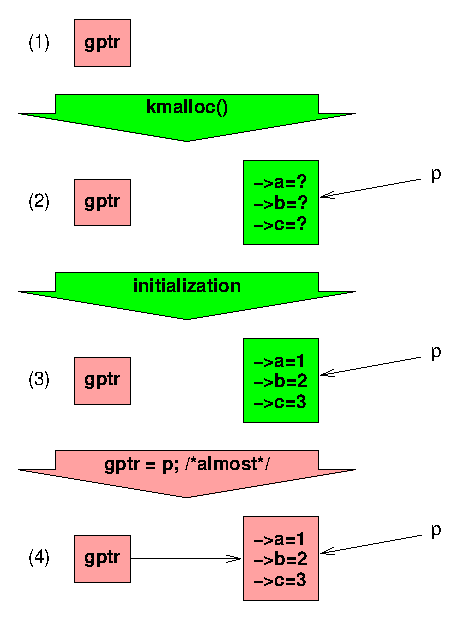
\includegraphics{defer/RCUListInsertClassic}}
\caption{Insertion With Concurrent Readers}
\label{fig:defer:Insertion With Concurrent Readers}
\end{figure}

To minimize implementability concerns, we focus on a minimal
data structure, which consists of a single global pointer that is either
\co{NULL} or references a single structure.
Minimal though it might be, this data structure is heavily used in
production~\cite{GeoffRomer2018C++DeferredReclamationP0561R4}.
A classic approach for insertion is shown in
\cref{fig:defer:Insertion With Concurrent Readers},
which shows four states with time advancing from top to bottom.
The first row shows the initial state, with \co{gptr} equal to \co{NULL}.
In the second row, we have allocated a structure which is uninitialized,
as indicated by the question marks.
In the third row, we have initialized the structure.
Finally, in the fourth and final row, we have updated \co{gptr} to
reference the newly allocated and initialized element.

We might hope that this assignment to \co{gptr} could use a simple
C-language assignment statement.
Unfortunately,
\cref{sec:toolsoftrade:Shared-Variable Shenanigans}
dashes these hopes.
Therefore, the updater cannot use a simple C-language assignment, but
must instead use \co{smp_store_release()} as shown in the figure,
or, as will be seen, \co{rcu_assign_pointer()}.

Similarly, one might hope that readers could use a single C-language
assignment to fetch the value of \co{gptr}, and be guaranteed to either
get the old value of \co{NULL} or to get the newly installed pointer,
but either way see a valid result.
Unfortunately, \cref{sec:toolsoftrade:Shared-Variable Shenanigans}
dashes these hopes as well.
To obtain this guarantee, readers must instead use \co{READ_ONCE()},
or, as will be seen, \co{rcu_dereference()}.
However, on most modern computer systems, each of these read-side primitives
can be implemented with a single load instruction, exactly the instruction
that would normally be used in single-threaded code.

\begin{listing}[tb]
\small
\fvset{numbers=left,numbersep=5pt,fontsize=\scriptsize,frame=single,xleftmargin=15pt,xrightmargin=5pt}
{\renewcommand{\theFancyVerbLine}{%
  {\rmfamily\tiny A\arabic{FancyVerbLine}}}
\begin{Verbatim}
 p = gp;
 do_something_with(p->a);
 do_something_with(p->b);
\end{Verbatim}
}
Might be transformed to:
{\renewcommand{\theFancyVerbLine}{%
  {\rmfamily\tiny B\arabic{FancyVerbLine}}}
\begin{Verbatim}
 p = gp;
 do_something_with(p->a);
 p = gp;
 do_something_with(p->b);
\end{Verbatim}
}
The compiler assumes normal variables do not spontaneously change,
\co{do_something_with()} might use many machine registers, and this
transformation reduces register pressure.
But if some other thread changes \co{gp} between lines~B1 and~B3 of the
transformed code, the values of \co{p->a} and \co{p->b} will be mismatched.
Prevent this by using \co{rcu_dereference()} as follows:
{\renewcommand{\theFancyVerbLine}{%
  {\rmfamily\tiny C\arabic{FancyVerbLine}}}
\begin{Verbatim}
 p = rcu_dereference(gp);
 do_something_with(p->a);
 do_something_with(p->b);
\end{Verbatim}
}
\caption{Compilers Can Reload Values}
\label{lst:defer:Compilers Can Reload Values}
\end{listing}

\begin{listing}[tb]
\small
\fvset{numbers=left,numbersep=5pt,fontsize=\scriptsize,frame=single,xleftmargin=15pt,xrightmargin=5pt}
{\renewcommand{\theFancyVerbLine}{%
  {\rmfamily\tiny A\arabic{FancyVerbLine}}}
\begin{Verbatim}
 p = malloc(sizeof(*p));
 p->a = compute_value();
 p->b = 42;
 gp = p;
\end{Verbatim}
}
Might be transformed to:
{\renewcommand{\theFancyVerbLine}{%
  {\rmfamily\tiny B\arabic{FancyVerbLine}}}
\begin{Verbatim}
 p = malloc(sizeof(*p));
 gp = p;
 p->a = compute_value();
 p->b = 42;
\end{Verbatim}
}
The compiler assumes normal variables are not concurrently accessed,
and thus that the order of stores does not matter.
If \co{compute_value()} was inlined, this transformation might produce
better code.
In this example, if some other thread loads \co{gp} immediately after
line~B2 of the transformed code, that thread might see pre-initialization
garbage in \co{p->a} and \co{p->b}.
Prevent this by using \co{rcu_assign_pointer()} as follows:
{\renewcommand{\theFancyVerbLine}{%
  {\rmfamily\tiny C\arabic{FancyVerbLine}}}
\begin{Verbatim}
 p = malloc(sizeof(*p));
 p->a = compute_value();
 p->b = 42;
 rcu_assign_pointer(gp, p);
\end{Verbatim}
}
\caption{Compilers Can Reorder Accesses}
\label{lst:defer:Compilers Can Reorder Accesses}
\end{listing}

To see the need for \co{rcu_dereference()}, please see lines~A1--A3 of
\cref{lst:defer:Compilers Can Reload Values}.
Here, the compiler may assume that \co{gp} retains the same value
throughout.
If \co{do_something_with()} uses many machine registers, then the
compiler might transform this code to the form shown in lines~B1--B4 of
this listing, thus avoiding the need to dedicate a register to the value
loaded from \co{gp}, but also possibly passing values from two
different structures to the pair of calls to \co{do_something_with()}
on lines~B2 and~B4.
This transformation would fatally confuse any implementation of
\co{do_something_with()} that assumed that it was being passed values
from the same structure.
To prevent this transformation, use \co{rcu_dereference()} as
shown on lines~C1--C3 of this listing, thus informing the compiler of the
possibility of concurrent updates to \co{gp}.

To see the need for \co{rcu_assign_pointer()}, please see lines~A1--A4 of
\cref{lst:defer:Compilers Can Reorder Accesses},
in which the compiler may assume that \co{gp} is not concurrently accessed
at all.
If \co{compute_value()} is inlined, the compiler might generate better
code by pulling the assignment to \co{gp} from line~A4 to follow line~A1,
as shown in the transformed code on lines~B1--B4.
If some other thread were to load fields \co{gp->a} or \co{gp->b} between
the store on line~B2 and the initializations on lines~B3 and~B4, that
other thread's acceses would return pre-initialization garbage.
You can prevent this transformation by using \co{rcu_assign_pointer()}
as shown on lines~C1--C4, thus informing the compiler of the possibility
of concurrent accesses to \co{gp} and of the need to preserve ordering.

Reviewing \cref{fig:defer:Insertion With Concurrent Readers}
from the viewpoint of readers, in the first three states all readers
see \co{gptr} having the value \co{NULL}.
Upon entering the fourth state, some readers might see \co{gptr} still
having the value \co{NULL} while others might see it referencing the
newly inserted element, but after some time, all readers will see this
new element.
At all times, all readers will see \co{gptr} as containing a valid pointer.
Therefore, it really is possible to add new data to linked data structures
while allowing concurrent readers to execute the same sequence of machine
instructions that is normally used in single-threaded code.
This no-cost approach to concurrent reading provides excellent performance
and scalability, and also is eminently suitable for real-time use.

\begin{figure}
\centering
\resizebox{3in}{!}{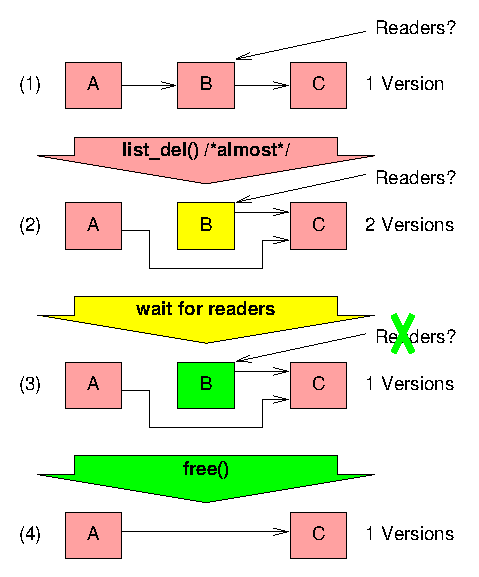
\includegraphics{defer/RCUListDeleteClassic}}
\caption{Deletion With Concurrent Readers}
\label{fig:defer:Deletion With Concurrent Readers}
\end{figure}

Insertion is of course quite useful, but sooner or later, it will also
be necessary to delete data.
As can be seen in
\cref{fig:defer:Deletion With Concurrent Readers},
the first step is easy.
Again taking the lessons from
\cref{sec:toolsoftrade:Shared-Variable Shenanigans}
to heart, \co{smp_store_release()} is used to \co{NULL} the pointer,
thus moving from the first row to the second in the figure.
At this point, pre-existing readers see the old structure with
\co{->addr} of~42 and \co{->iface} of~1, but new readers will see
a \co{NULL} pointer, that is, concurrent readers can disagree on
the state, as indicated by the ``2~Versions'' in the figure.

\QuickQuizSeries{%
\QuickQuizB{
	Why does
	\cref{fig:defer:Deletion With Concurrent Readers}
	use \co{smp_store_release()} given that it is storing
	a \co{NULL} pointer?
	Wouldn't \co{WRITE_ONCE()} work just as well in this case,
	given that there is no structure initialization to order
	against the store of the \co{NULL} pointer?
}\QuickQuizAnswerB{
	Yes, it would.

	Because a \co{NULL} pointer is being assigned, there is nothing
	to order against, so there is no need for \co{smp_store_release()}.
	In contrast, when assigning a non-\co{NULL} pointer, it is
	necessary to use \co{smp_store_release()} in order to ensure
	that initialization of the pointed-to structure is carried
	out before assignment of the pointer.

	In short, \co{WRITE_ONCE()} would work, and would
	save a little bit of CPU time on some architectures.
	However, as we will see, software-engineering concerns
	will motivate use of a special \co{rcu_assign_pointer()}
	that is quite similar to \co{smp_store_release()}.
}\QuickQuizEndB
%
\QuickQuizE{
	Readers running concurrently with each other and with the procedure
	outlined in
	\cref{fig:defer:Deletion With Concurrent Readers}
	can disagree on the value of \co{gptr}.
	Isn't that just a wee bit problematic???
}\QuickQuizAnswerE{
	Not necessarily.

	As hinted at in
	\cref{sec:cpu:Hardware Optimizations,sec:cpu:Hardware Free Lunch?},
	speed-of-light delays mean that a computer's data is always
	stale compared to whatever external reality that data is intended
	to model.

	Real-world algorithms therefore absolutely must tolerate
	inconsistencies between external reality and the in-computer
	data reflecting that reality.
	Many of those algorithms are also able to tolerate some degree
	of inconsistency within the in-computer data.
	\Cref{sec:datastruct:RCU-Protected Hash Table Discussion}
	discusses this point in more detail.

	Please note that this need to tolerate inconsistent and stale
	data is not limited to RCU\@.
	It also applies to reference counting, hazard pointers, sequence
	locks, and even to some locking use cases.
	For example, if you compute some quantity while holding a lock,
	but use that quantity after releasing that lock,
	you might well be using stale data.
	After all, the data that quantity is based on might change
	arbitrarily as soon as the lock is released.

	So yes, RCU readers can see stale and inconsistent data, but no,
	this is not necessarily problematic.
	And, when needed, there are RCU usage patterns that avoid both
	staleness and inconsistency~\cite{Arcangeli03}.
}\QuickQuizEndE
}

We get back to a single version simply by waiting for all the
pre-existing readers to complete, as shown in row~3.\footnote{
	Which means that the wait-for-readers property introduced in
	\cref{sec:defer:Read-Copy Update (RCU)}
	really did have an important use after all!}
At that point, all the pre-existing readers are done, and no later
reader has a path to the old data item, so there can no longer be
any readers referencing it.
It may therefore be safely freed, as shown on row~4.

Thus, given a way to wait for pre-existing readers to complete,
it is possible to both add data to and remove data from a linked
data structure, despite the readers executing the same sequence
of machine instructions that would be appropriate for single-threaded
execution.
So perhaps going all the way was not too far after all!

But how can we tell when all of the pre-existing readers have in
fact completed?
This question is the topic of \cref{sec:defer:Waiting for Readers}.
But first, the next section defines RCU's core API.

\subsubsection{Core RCU API}
\label{sec:defer:Core RCU API}

The full Linux-kernel API is quite extensive, with more than one
hundred API members.
However, this section will confine itself to six core RCU API members,
which suffices for the upcoming sections introducing RCU and covering
its fundamentals.
The full API is covered in \cref{sec:defer:RCU Linux-Kernel API}.

Three members of the core APIs are used by readers.
The \apik{rcu_read_lock()} and \apik{rcu_read_unlock()} functions delimit
\IXhmrpl{RCU read-side}{critical section}.
These may be nested, so that one \co{rcu_read_lock()}--\co{rcu_read_unlock()}
pair can be enclosed within another.
In this case, the nested set of RCU read-side critical sections act as
one large critical section covering the full extent of the nested set.
The third read-side API member, \apik{rcu_dereference()}, fetches an
\IXr{RCU-protected pointer}.
Conceptually, \co{rcu_dereference()} simply loads from memory, but we
will see in
\cref{sec:defer:Publish-Subscribe Mechanism}
that \co{rcu_dereference()} must prevent the compiler and (in
one case) the CPU from reordering its load with later memory operations
that dereference this pointer.

\QuickQuiz{
	What is an RCU-protected pointer?
}\QuickQuizAnswer{
	A pointer to \IXr{RCU-protected data}.
	RCU-protected data is in turn a block of dynamically allocated
	memory whose freeing will be deferred such that an RCU grace
	period will elapse between the time that there were no longer
	any RCU-reader-accessible pointers to that block and the time
	that that block is freed.
	This ensures that no RCU readers will have access to that block at
	the time that it is freed.

	RCU-protected pointers must be handled carefully.
	For example, any reader that intends to dereference an
	RCU-protected pointer must use \co{rcu_dereference()} (or
	stronger) to load that pointer.
	In addition, any updater must use \co{rcu_assign_pointer()}
	(or stronger) to store to that pointer.
}\QuickQuizEnd

The other three members of the core APIs are used by updaters.
The \apik{synchronize_rcu()} function implements the ``wait for readers''
operation from \cref{fig:defer:Deletion With Concurrent Readers}.
The \apik{call_rcu()} function is the asynchronous counterpart of
\co{synchronize_rcu()} by invoking the specified function after
all pre-existing RCU readers have completed.
Finally, the \apik{rcu_assign_pointer()} macro is used to update an
RCU-protected pointer.
Conceptually, this is simply an assignment statement, but we will
see in
\cref{sec:defer:Publish-Subscribe Mechanism}
that \co{rcu_assign_pointer()} must prevent the compiler and the CPU
from reordering this assignment to precede any prior assignments used
to initialize the pointed-to structure.

\begin{table*}
\renewcommand*{\arraystretch}{1.25}
\rowcolors{2}{}{lightgray}
\small
\centering
\ebresizewidth{
\begin{tabular}{llp{2.4in}}
\toprule
&
	Primitive &
		Purpose \\
\midrule
\cellcolor{white}\emph{Readers} &
	\tco{rcu_read_lock()} &
		Start an RCU read-side critical section. \\
&
	\tco{rcu_read_unlock()} &
		End an RCU read-side critical section. \\
\cellcolor{white}&
	\tco{rcu_dereference()} &
		Safely load an RCU-protected pointer. \\
\midrule
\emph{Updaters} &
	\tco{synchronize_rcu()} &
		Wait for all pre-existing RCU read-side critical sections to
		complete. \\
\cellcolor{white}&
	\tco{call_rcu()} &
		Invoke the specified function after all pre-existing RCU read-side
		critical sections complete. \\
&
	\tco{rcu_assign_pointer()} &
		Safely update an RCU-protected pointer. \\
\bottomrule
\end{tabular}
}
\caption{Core RCU API}
\label{tab:defer:Core RCU API}
\end{table*}

\QuickQuiz{
	What does \co{synchronize_rcu()} do if it starts at about
	the same time as an \co{rcu_read_lock()}?
}\QuickQuizAnswer{
	If a \co{synchronize_rcu()} cannot prove that it started
	before a given \co{rcu_read_lock()}, then it must wait
	for the corresponding \co{rcu_read_unlock()}.
}\QuickQuizEnd

The core RCU API is summarized in \cref{tab:defer:Core RCU API} for
easy reference.
With that, we are ready to continue this introduction to RCU with
the key RCU operation, waiting for readers.

\subsubsection{Waiting for Readers}
\label{sec:defer:Waiting for Readers}

It is tempting to base the reader-waiting functionality of
\co{synchronize_rcu()} and \co{call_rcu()} on a reference counter
updated by \co{rcu_read_lock()} and \co{rcu_read_unlock()}, but
\cref{fig:count:Atomic Increment Scalability on x86}
in
\cref{chp:Counting}
shows that concurrent reference counting results in extreme overhead.
This extreme overhead was confirmed in the specific case of
reference counters in
\cref{fig:defer:Pre-BSD Routing Table Protected by Reference Counting}
on
\cpageref{fig:defer:Pre-BSD Routing Table Protected by Reference Counting}.
Hazard pointers profoundly reduce this overhead, but, as we saw in
\cref{fig:defer:Pre-BSD Routing Table Protected by Hazard Pointers}
on
\cpageref{fig:defer:Pre-BSD Routing Table Protected by Hazard Pointers},
not to zero.
Nevertheless, many RCU implementations use counters with carefully
controlled cache locality.

A second approach observes that memory synchronization is expensive,
and therefore uses registers instead, namely each CPU's or thread's
program counter (PC), thus imposing no overhead on readers, at least
in the absence of concurrent updates.
The updater polls each relevant PC, and if that PC is not within read-side
code, then the corresponding CPU or thread is within a quiescent state,
in turn signaling the completion of any reader that might have access
to the newly removed data element.
Once all CPU's or thread's PCs have been observed to be outside of any
reader, the \IX{grace period} has completed.
Please note that this approach poses some serious challenges, including
memory ordering, functions that are \emph{sometimes} invoked from readers,
and ever-exciting code-motion optimizations.
Nevertheless, this approach is said to be used in
production~\cite{MikeAsh2015Apple}.

A third approach is to simply wait for a fixed period of time that is
long enough to comfortably exceed the lifetime of any reasonable
reader~\cite{Jacobson93,AjuJohn95}.
This can work quite well in hard real-time systems~\cite{YuxinRen2018RTRCU},
but in less exotic
settings, Murphy says that it is critically important to be prepared
even for unreasonably long-lived readers.
To see this, consider the consequences of failing to do so:
A data item will be freed while the unreasonable reader is still
referencing it, and that item might well be immediately reallocated,
possibly even as a data item of some other type.
The unreasonable reader and the unwitting reallocator would then
be attempting to use the same memory for two very different purposes.
The ensuing mess will be exceedingly difficult to debug.
Nevertheless, \ppl{Paul}{Khuong} reports that this approach is
occasionally used in production, which can work acceptably well when the
fixed period of time is long enough, or when a failure rate is
acceptable.\footnote{
	Paul Khuong also reports that in the case he knows best, they
	eventually transitioned to a more principled approach.}

A fourth approach is to wait forever, secure in the knowledge that
doing so will accommodate even the most unreasonable reader.
This approach is also called ``leaking memory'', and has a bad reputation
due to the fact that memory leaks often require untimely and
inconvenient reboots.
Nevertheless, this is a viable strategy when the update rate and the
uptime are both sharply bounded.
For example, this approach could work well in a high-availability
cluster where systems were periodically crashed in order to ensure
that cluster really remained highly available.\footnote{
	The program that forces the periodic crashing is sometimes
	known as a ``chaos monkey'':
	\url{https://netflix.github.io/chaosmonkey/}.
	However, it might also be a mistake to neglect chaos caused
	by systems running for too long.}
Leaking the memory is also a viable strategy in environments having
garbage collectors, in which case the garbage collector can be thought
of as plugging the leak~\cite{Kung80}.
However, if your environment lacks a garbage collector, read on!

A fifth approach avoids the periodic crashes in favor of periodically
``stopping the world'', as exemplified by the traditional stop-the-world
garbage collector.
This approach was also heavily used during the decades before
ubiquitous connectivity, when it was common practice to power systems
off at the end of each working day.
However, in today's always-connected always-on world, stopping the world
can gravely degrade response times, which has been one motivation for the
development of concurrent garbage collectors~\cite{DavidFBacon2003RTGC}.
Furthermore, although we need all pre-existing readers to complete, we do
not need them all to complete at the same time.

This observation leads to the sixth approach, which is stopping
one CPU or thread at a time.
This approach has the advantage of not degrading reader response times
at all, let alone gravely.
Furthermore, numerous applications already have states (termed
\emph{\IXpl{quiescent state}}) that can be
reached only after all pre-existing readers are done.
In transaction-processing systems, the time between a pair of
successive transactions might be a quiescent state.
In reactive systems, the state between a pair of successive events
might be a quiescent state.
Within non-preemptive operating-systems kernels, a context switch can be
a quiescent state~\cite{McKenney98}.
Either way, once all CPUs and/or threads have passed through a quiescent
state, the system is said to have completed a \emph{grace period},
at which point all readers in existence at the start of that grace period
are guaranteed to have completed.
As a result, it is also guaranteed to be safe to free any removed data
items that were removed prior to the start of that grace period.\footnote{
	It is possible to do much more with RCU than simply defer
	reclamation of memory, but deferred reclamation is RCU's most
	common use case, and is therefore an excellent place to start.
	For an example of the more general case of deferred execution,
	please see phased state change in \cref{sec:defer:Phased State
	Change}.}

Within a non-preemptive operating-system kernel, for a context switch to be
a valid quiescent state, readers must be prohibited from blocking while
referencing a given instance of the data structure obtained via the \co{gptr}
pointer shown in
\cref{fig:defer:Insertion With Concurrent Readers,%
fig:defer:Deletion With Concurrent Readers}.
This no-blocking constraint is consistent with similar constraints
on pure spinlocks, where a CPU is forbidden from blocking while
holding a spinlock.
Without this constraint, all CPUs might be consumed by threads
spinning attempting to acquire a spinlock held by a blocked thread.
The spinning threads will not relinquish their CPUs until they acquire
the lock, but the thread holding the lock cannot possibly release it
until one of the spinning threads relinquishes a CPU\@.
This is a classic deadlock situation, and this \IX{deadlock} is avoided
by forbidding blocking while holding a spinlock.

Again, this same constraint is imposed on reader threads dereferencing
\co{gptr}:
Such threads are not allowed to block until after
they are done using the pointed-to data item.
Returning to the second row of
\cref{fig:defer:Deletion With Concurrent Readers},
where the updater has just completed executing the \co{smp_store_release()},
imagine that CPU~0 executes a context switch.
Because readers are not permitted to block while traversing the linked
list, we are guaranteed that all prior readers that might have been running on
CPU~0 will have completed.
Extending this line of reasoning to the other CPUs, once each CPU has
been observed executing a context switch, we are guaranteed that all
prior readers have completed, and that there are no longer any reader
threads referencing the newly removed data element.
The updater can then safely free that data element, resulting in the
state shown at the bottom of
\cref{fig:defer:Deletion With Concurrent Readers}.

\begin{figure}
\centering
\resizebox{3in}{!}{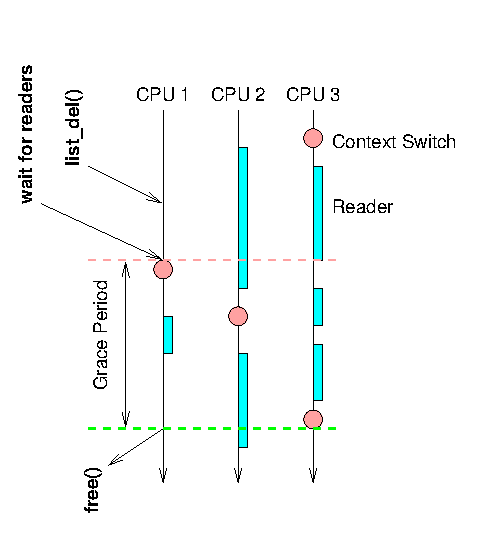
\includegraphics{defer/QSBRGracePeriod}}
\caption{QSBR\@:
		 Waiting for Pre-Existing Readers}
\label{fig:defer:QSBR: Waiting for Pre-Existing Readers}
\end{figure}

This approach is termed \IXacrfst{qsbr}~\cite{ThomasEHart2006a}.
A QSBR schematic is shown in
\cref{fig:defer:QSBR: Waiting for Pre-Existing Readers},
with time advancing from the top of the figure to the bottom.
The cyan-colored boxes depict RCU read-side critical sections,
each of which begins with \co{rcu_read_lock()} and ends with
\co{rcu_read_unlock()}.
CPU~1 does the \co{WRITE_ONCE()} that removes the current data
item (presumably having previously read the pointer value and
availed itself of appropriate synchronization), then waits
for readers.
This wait operation results in an immediate context switch, which is a
quiescent state (denoted by the pink circle), which in turn means that
all prior reads on CPU~1 have completed.
Next, CPU~2 does a context switch, so that all readers on CPUs~1 and~2
are now known to have completed.
Finally, CPU~3 does a context switch.
At this point, all readers throughout the entire system are known to have
completed, so the grace period ends, permitting \co{synchronize_rcu()} to
return to its caller, in turn permitting CPU~1 to free the old data item.

\QuickQuiz{
	In \cref{fig:defer:QSBR: Waiting for Pre-Existing Readers},
	the last of CPU~3's readers that could possibly have
	access to the old data item ended before the grace period
	even started!
	So why would anyone bother waiting until CPU~3's later context
	switch???
}\QuickQuizAnswer{
	Because that waiting is exactly what enables readers to use
	the same sequence of instructions that is appropriate for
	single-theaded situations.
	In other words, this additional ``redundant'' waiting enables
	excellent read-side performance, scalability, and real-time
	response.
}\QuickQuizEnd

\subsubsection{Toy Implementation}
\label{sec:defer:Toy Implementation}

Although production-quality QSBR implementations can be quite complex,
a toy non-preemptive Linux-kernel implementation is quite simple:

\begin{VerbatimN}[samepage=true]
void synchronize_rcu(void)
{
	int cpu;

	for_each_online_cpu(cpu)
		sched_setaffinity(current->pid, cpumask_of(cpu));
}
\end{VerbatimN}

The \co{for_each_online_cpu()} primitive iterates over all CPUs, and
the \co{sched_setaffinity()} function causes the current thread to
execute on the specified CPU, which forces the destination CPU to execute
a context switch.
Therefore, once the \co{for_each_online_cpu()} has completed, each CPU
has executed a context switch, which in turn guarantees that
all pre-existing reader threads have completed.

\begin{listing}
\begin{fcvlabel}[ln:defer:Insertion and Deletion With Concurrent Readers]
\begin{VerbatimL}[commandchars=\\\[\]]
struct route *gptr;

int access_route(int (*f)(struct route *rp))
{
	int ret = -1;
	struct route *rp;

	rcu_read_lock();
	rp = rcu_dereference(gptr);
	if (rp)
		ret = f(rp);		\lnlbl[access_rp]
	rcu_read_unlock();
	return ret;
}

struct route *ins_route(struct route *rp)
{
	struct route *old_rp;

	spin_lock(&route_lock);
	old_rp = gptr;
	rcu_assign_pointer(gptr, rp);
	spin_unlock(&route_lock);
	return old_rp;
}

int del_route(void)
{
	struct route *old_rp;

	spin_lock(&route_lock);
	old_rp = gptr;
	RCU_INIT_POINTER(gptr, NULL);
	spin_unlock(&route_lock);
	synchronize_rcu();
	free(old_rp);
	return !!old_rp;
}
\end{VerbatimL}
\end{fcvlabel}
\caption{Insertion and Deletion With Concurrent Readers}
\label{lst:defer:Insertion and Deletion With Concurrent Readers}
\end{listing}

Please note that this approach is \emph{not} production quality.
Correct handling of a number of corner cases and the need for a number
of powerful optimizations mean that production-quality implementations
are quite complex.
In addition, RCU implementations for preemptible environments
require that readers actually do something, which in non-real-time
Linux-kernel environments can be as simple as defining
\co{rcu_read_lock()} and \co{rcu_read_unlock()} as \co{preempt_disable()}
and \co{preempt_enable()}, respectively.\footnote{
	Some toy RCU implementations that handle preempted
	read-side critical sections are shown in
	\cref{chp:app:``Toy'' RCU Implementations}\@.}
However, this simple non-preemptible approach is conceptually complete,
and demonstrates that it really is possible to provide read-side
synchronization at zero cost, even in the face of concurrent updates.
In fact,
\cref{lst:defer:Insertion and Deletion With Concurrent Readers}
shows how reading (\co{access_route()}),
\cref{fig:defer:Insertion With Concurrent Readers}'s
insertion (\co{ins_route()}) and
\cref{fig:defer:Deletion With Concurrent Readers}'s
deletion (\co{del_route()}) can
be implemented.
(A slightly more capable routing table is shown in
\cref{sec:defer:RCU for Pre-BSD Routing}.)

\QuickQuizSeries{%
\QuickQuizB{
	What is the point of \co{rcu_read_lock()} and \co{rcu_read_unlock()} in
	\cref{lst:defer:Insertion and Deletion With Concurrent Readers}?
	Why not just let the quiescent states speak for themselves?
}\QuickQuizAnswerB{
	Recall that readers are not permitted to pass through a quiescent
	state.
	For example, within the Linux kernel, RCU readers are not permitted
	to execute a context switch.
	Use of \co{rcu_read_lock()} and \co{rcu_read_unlock()} enables
	debug checks for improperly placed quiescent states, making it
	easy to find bugs that would otherwise be difficult to find,
	intermittent, and quite destructive.
}\QuickQuizEndB
%
\QuickQuizE{
	What is the point of \co{rcu_dereference()}, \co{rcu_assign_pointer()}
	and \co{RCU_INIT_POINTER()} in
	\cref{lst:defer:Insertion and Deletion With Concurrent Readers}?
	Why not just use \co{READ_ONCE()}, \co{smp_store_release()}, and
	\co{WRITE_ONCE()}, respectively?
}\QuickQuizAnswerE{
	The RCU-specific APIs do have similar semantics to the suggested
	replacements, but also enable static-analysis debugging checks
	that complain if an RCU-specific API is invoked on a non-RCU
	pointer and vice versa.
}\QuickQuizEndE
}

Referring back to
\cref{lst:defer:Insertion and Deletion With Concurrent Readers},
note that \co{route_lock} is used to synchronize between concurrent updaters
invoking \co{ins_route()} and \co{del_route()}.
However, this lock is not acquired by readers invoking \co{access_route()}:
Readers are instead protected by the QSBR techniques described in
\cref{sec:defer:Waiting for Readers}.

Note that \co{ins_route()} simply returns the old value of \co{gptr}, which
\cref{fig:defer:Insertion With Concurrent Readers} assumed would
always be \co{NULL}.
This means that it is the caller's responsibility to figure out what to
do with a non-\co{NULL} value, a task complicated by the fact that
readers might still be referencing it for an indeterminate period of time.
Callers might use one of the following approaches:

\begin{enumerate}
\item	Use \co{synchronize_rcu()} to safely free the pointed-to structure.
	Although this approach is correct from an RCU perspective, it
	arguably has software-engineering leaky-API problems.
\item	Trip an assertion if the returned pointer is non-\co{NULL}.
\item	Pass the returned pointer to a later invocation of
	\co{ins_route()} to restore the earlier value.
\end{enumerate}

In contrast, \co{del_route()} uses \co{synchronize_rcu()} and
\co{free()} to safely free the newly deleted data item.

\QuickQuiz{
	But what if the old structure needs to be freed, but the caller
	of \co{ins_route()} cannot block, perhaps due to performance
	considerations or perhaps because the caller is executing within
	an RCU read-side critical section?
}\QuickQuizAnswer{
	A \co{call_rcu()} function, which is described in
	\cref{sec:defer:Wait For Pre-Existing RCU Readers},
	permits asynchronous grace-period waits.
}\QuickQuizEnd

This example shows one general approach to reading and updating
RCU-protected data structures, however, there is quite a variety
of use cases, several of which are covered in
\cref{sec:defer:RCU Usage}.

In summary, it is in fact possible to create concurrent linked data
structures that can be traversed by readers executing the same sequence
of machine instructions that would be executed by single-threaded readers.
The next section summarizes RCU's high-level properties.

\subsubsection{RCU Properties}
\label{sec:defer:RCU Properties}

A key RCU property is that reads need not wait for updates.
This property enables RCU implementations to provide low-cost or even
no-cost readers, resulting in low overhead and excellent scalability.
This property also allows RCU readers and updaters to make useful
concurrent forward progress.
In contrast, conventional synchronization primitives must enforce strict
mutual exclusion using expensive instructions, thus increasing overhead
and degrading scalability, but also typically prohibiting readers and
updaters from making useful concurrent forward progress.

\QuickQuiz{
	Doesn't \cref{sec:defer:Sequence Locks}'s seqlock
	also permit readers and updaters to make useful concurrent
	forward progress?
}\QuickQuizAnswer{
	Yes and no.
	Although seqlock readers can run concurrently with
	seqlock writers, whenever this happens, the \co{read_seqretry()}
	primitive will force the reader to retry.
	This means that any work done by a seqlock reader running concurrently
	with a seqlock updater will be discarded and then redone upon retry.
	So seqlock readers can \emph{run} concurrently with updaters,
	but they cannot actually get any work done in this case.

	In contrast, RCU readers can perform useful work even in presence
	of concurrent RCU updaters.

	However, both reference counters
	(\cref{sec:defer:Reference Counting})
	and hazard pointers
	(\cref{sec:defer:Hazard Pointers})
	really do permit useful concurrent forward progress for both
	updaters and readers, just at somewhat greater cost.
	Please see
	\cref{sec:defer:Which to Choose?}
	for a comparison of these different solutions to the
	deferred-reclamation problem.
}\QuickQuizEnd

As noted earlier, RCU delimits readers with \co{rcu_read_lock()} and
\co{rcu_read_unlock()}, and ensures that each reader has a coherent view
of each object (see \cref{fig:defer:Deletion With Concurrent Readers}) by
maintaining multiple versions of objects and using update-side primitives
such as \co{synchronize_rcu()} to ensure that objects are not
freed until after the completion of all readers that might be using them.
RCU uses \co{rcu_assign_pointer()} and \co{rcu_dereference()} to provide
efficient and scalable mechanisms for publishing and reading new versions
of an object, respectively.
These mechanisms distribute the work among read and
update paths in such a way as to make read paths extremely fast, using
replication and weakening optimizations in a manner similar to
\IXpl{hazard pointer}, but without the need for read-side retries.
In some cases, including \co{CONFIG_PREEMPT=n} Linux kernels,
RCU's read-side primitives have zero overhead.

But are these properties actually useful in practice?
This question is taken up by the next section.

\subsubsection{Practical Applicability}
\label{sec:defer:Practical Applicability}

\begin{figure}
\centering
\resizebox{3in}{!}{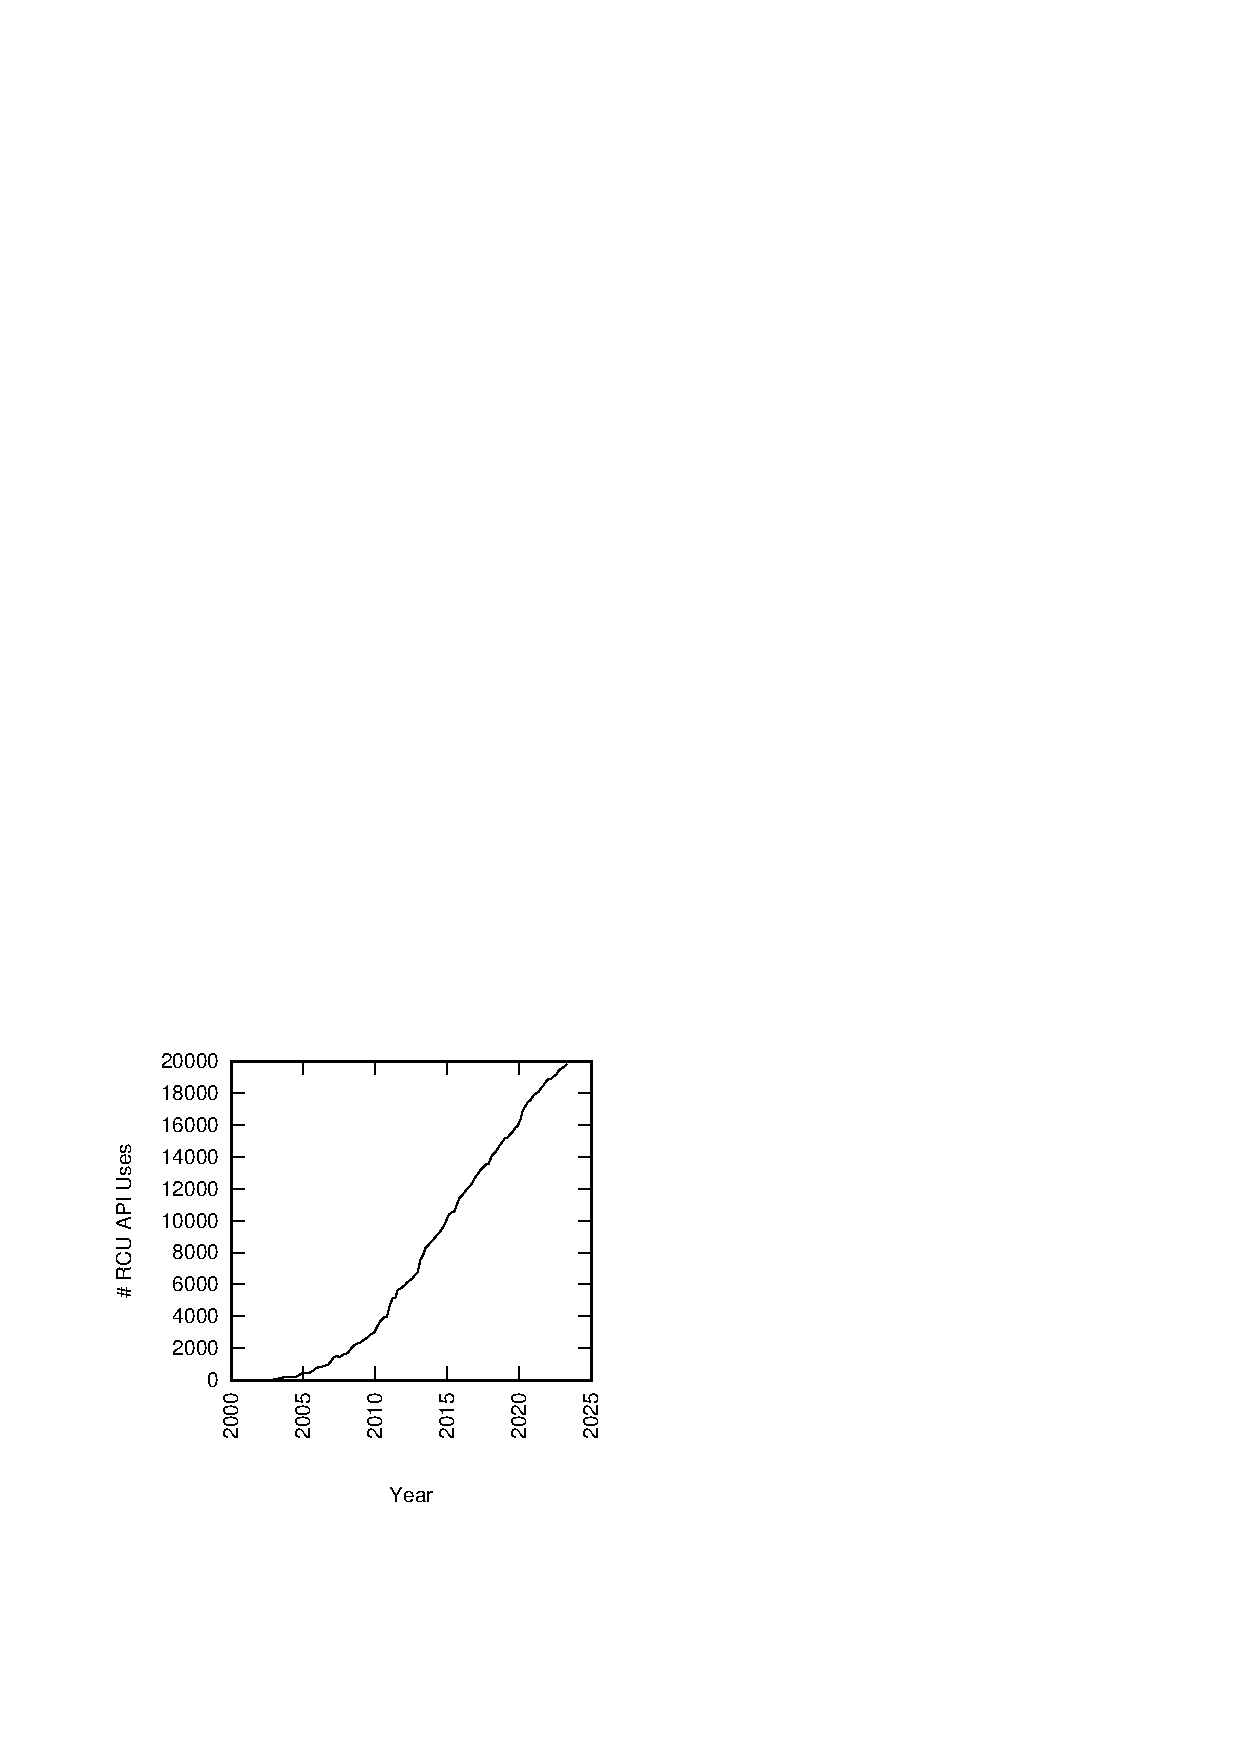
\includegraphics{defer/linux-RCU}}
\caption{RCU Usage in the Linux Kernel}
\label{fig:defer:RCU Usage in the Linux Kernel}
\end{figure}

RCU has been used in the Linux kernel since
October 2002~\cite{Torvalds2.5.43}.
Use of the RCU API has increased substantially since that time,
as can be seen in
\cref{fig:defer:RCU Usage in the Linux Kernel}.
RCU has enjoyed heavy use both prior to and since its acceptance
in the Linux kernel, as discussed in
\cref{sec:defer:RCU Related Work}.
In short, RCU enjoys wide practical applicability.

The minimal example discussed in this section is a good introduction to RCU\@.
However, effective use of RCU often requires that you think differently
about your problem.
It is therefore useful to examine RCU's fundamentals, a task taken up
by the following section.

% defer/rcufundamental.tex
% mainfile: ../perfbook.tex
% SPDX-License-Identifier: CC-BY-SA-3.0

\subsection{RCU Fundamentals}
\label{sec:defer:RCU Fundamentals}
\OriginallyPublished{sec:defer:RCU Fundamentals}{RCU Fundamentals}{Linux Weekly News}{PaulEMcKenney2007WhatIsRCUFundamentally}

This section re-examines the ground covered in the previous section, but
independent of any particular example or use case.
People who prefer to live their lives very close to the actual code may
wish to skip the underlying fundamentals presented in this section.

The common use of RCU to protect linked data structures is comprised
of three fundamental mechanisms, the first being used for insertion,
the second being used for deletion, and the third being used to allow
readers to tolerate concurrent insertions and deletions.
\Cref{sec:defer:Publish-Subscribe Mechanism}
describes the publish-subscribe mechanism used for insertion,
\cref{sec:defer:Wait For Pre-Existing RCU Readers}
describes how waiting for pre-existing RCU readers enables
deletion,\footnote{
	Yes, RCU being what it is, this most fundamental component of
	RCU is covered not first, but second.}
and
\cref{sec:defer:Maintain Multiple Versions of Recently Updated Objects}
discusses how maintaining multiple versions of recently updated objects
permits concurrent insertions and deletions.
Finally,
\cref{sec:defer:Summary of RCU Fundamentals}
summarizes RCU fundamentals.

\subsubsection{Publish-Subscribe Mechanism}
\label{sec:defer:Publish-Subscribe Mechanism}

Because RCU readers are not excluded by RCU updaters, an RCU-protected
data structure might change while a reader accesses it.
The accessed data item might be moved, removed, or replaced.
Because the data structure does not ``hold still'' for the reader,
each reader's access can be thought of as subscribing to the current
version of the RCU-protected data item.
For their part, updaters can be thought of as publishing new versions.

% @@@ Merge usage section into "Which to Choose?" and suggest choices.

\begin{figure}
\centering
\resizebox{3in}{!}{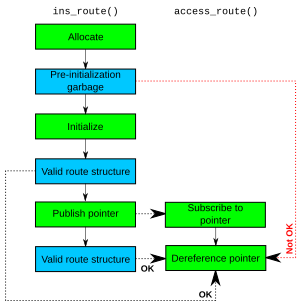
\includegraphics{defer/pubsub}}
\caption{Publication/Subscription Constraints}
\label{fig:defer:Publication/Subscription Constraints}
\end{figure}

Unfortunately, as laid out in
\cref{sec:toolsoftrade:Shared-Variable Shenanigans}
and reiterated in
\cref{sec:defer:Minimal Insertion and Deletion},
it is unwise to use \IXplx{plain access}{es} for these publication and subscription
operations.
It is instead necessary to inform both the compiler and the CPU
of the need for care, as can be seen from
\cref{fig:defer:Publication/Subscription Constraints},
which illustrates interactions between concurrent executions of
\co{ins_route()} (and its caller) and \co{access_route()} from
\cref{lst:defer:Insertion and Deletion With Concurrent Readers}.

The \co{ins_route()} column from
\cref{fig:defer:Publication/Subscription Constraints}
shows \co{ins_route()}'s caller allocating a new \co{route} structure,
which then contains pre-initialization garbage.
The caller then initializes the newly allocated structure, and then
invokes \co{ins_route()} to publish a pointer to the new \co{route}
structure.
Publication does not affect the contents of the structure, which
therefore remain valid after publication.

The \co{access_route()} column from this same figure shows
the pointer being subscribed to and dereferenced.
This dereference operation absolutely must see a valid \co{route}
structure rather than pre-initialization garbage because referencing
garbage could result in memory corruption, crashes, and hangs.
As noted earlier, avoiding such garbage means that the publish and
subscribe operations must inform both the compiler and the CPU of the
need to maintain the needed ordering.

Publication is carried out by \co{rcu_assign_pointer()}, which ensures that
\co{ins_route()}'s caller's initialization is ordered before the actual
publication operation's store of the pointer.
In addition, \co{rcu_assign_pointer()} must be atomic in the sense that 
concurrent readers see either the old value of the pointer or the new
value of the pointer, but not some mash-up of these two values.
These requirements are met by the C11 store-release operation, and in
fact in the Linux kernel, \co{rcu_assign_pointer()} is defined in terms
of \co{smp_store_release()}, which is similar to C11 store-release.

Note that if concurrent updates are required, some sort of synchronization
mechanism will be required to mediate among multiple concurrent
\co{rcu_assign_pointer()} calls on the same pointer.
In the Linux kernel, locking is the mechanism of choice, but pretty
much any synchronization mechanism may be used.
An example of a particularly lightweight synchronization mechanism is
\cref{chp:Data Ownership}'s data ownership:
If each pointer is owned by a particular thread, then that thread may
execute \co{rcu_assign_pointer()} on that pointer with no additional
synchronization overhead.

\QuickQuiz{
	Wouldn't use of data ownership for RCU updaters mean that
	the updates could use exactly the same sequence of instructions
	as would the corresponding single-threaded code?
}\QuickQuizAnswer{
	Sometimes, for example, on TSO systems such as x86 or the IBM
	mainframe where a store-release operation emits a single store
	instruction.
	However, weakly ordered systems must also emit a memory barrier
	or perhaps a store-release instruction.
	In addition, removing data requires quite a bit of additional
	work because it is necessary to wait for pre-existing readers
	before freeing the removed data.
}\QuickQuizEnd

Subscription is carried out by \co{rcu_dereference()}, which prevents
the compiler and (in one case) the CPU from reordering the pointer
load with later memory operations that dereference that pointer.
Similar to \co{rcu_assign_pointer()}, \co{rcu_dereference()} must be
atomic in the sense that the value loaded must be that from a single
store, for example, the compiler must not tear the load.\footnote{
	That is, the compiler must not break the load into multiple
	smaller loads, as described under ``load tearing'' in
	\cref{sec:toolsoftrade:Shared-Variable Shenanigans}.}
Unfortunately, compiler support for \co{rcu_dereference()} is at best
a work in progress~\cite{PaulEMcKennneyConsumeP0190R4,PaulEMcKenney2017markconsumeP0462R1,JFBastien2018P0750R1consume}.
In the meantime, the Linux kernel relies on volatile loads, the details of
the various CPU architectures, coding
restrictions~\cite{PaulEMcKenney2014rcu-dereference},
and, on DEC Alpha~\cite{ALPHA2002}, a memory-barrier instruction.
However, on other architectures, \co{rcu_dereference()} typically
emits a single load instruction, just as would the equivalent single-threaded
code.
The coding restrictions are described in more detail in
\cref{sec:memorder:Address- and Data-Dependency Difficulties},
however, the common case of field selection (\qtco{->}) works quite well.
Software that does not require the ultimate in read-side performance
can instead use C11 \IXpl{acquire load}, which provide the needed ordering and
more, albeit at a cost.
It is hoped that lighter-weight compiler support for \co{rcu_dereference()}
will appear in due course.

In short, use of \co{rcu_assign_pointer()} for publishing pointers and
use of \co{rcu_dereference()} for subscribing to them successfully avoids the
``Not OK'' garbage loads depicted in
\cref{fig:defer:Publication/Subscription Constraints}.
These two primitives can therefore be used to add new data to linked
structures without disrupting concurrent readers.

\QuickQuiz{
	But suppose that updaters are adding and removing multiple data
	items from a linked list while a reader is iterating over that
	same list.
	Specifically, suppose that a list initially contains elements
	A, B, and~C, and that an updater removes element A and then
	adds a new element D at the end of the list.
	The reader might well see \{A, B, C, D\}, when that sequence of
	elements never actually ever existed!
	In what alternate universe would that qualify as ``not disrupting
	concurrent readers''???
}\QuickQuizAnswer{
	In the universe where an iterating reader is only required to
	traverse elements that were present throughout the full duration
	of the iteration.
	In the example, that would be elements B and~C\@.
	Because elements A and~D were each present for only part of the
	iteration, the reader is permitted to iterate over them, but not
	obliged to.
	Note that this supports the common case where the reader is simply
	looking up a single item, and does not know or care about the
	presence or absence of other items.

	If stronger consistency is required, then higher-cost
	synchronization mechanisms are required, for example, sequence
	locking or reader-writer locking.
	But if stronger consistency is \emph{not} required (and it very often
	is not), then why pay the higher cost?
}\QuickQuizEnd

Adding data to a linked structure without disrupting readers is a good thing,
as are the cases where this can be done with no added read-side cost compared
to single-threaded readers.
However, in most cases it is also necessary to remove data, and this is the
subject of the next section.

\subsubsection{Wait For Pre-Existing RCU Readers}
\label{sec:defer:Wait For Pre-Existing RCU Readers}

The most basic component of RCU is waiting for things to finish.
Of course, there are a great many other ways of waiting for things to
finish, including reference counts, reader-writer locks, events, and so on.
The great advantage of RCU is that it can wait for each of
(say) 20,000 different things without having to explicitly
track each and every one of them, and without having to worry about
the performance degradation, scalability limitations, complex deadlock
scenarios, and memory-leak hazards that are inherent in schemes
using explicit tracking.

In RCU's case, each of the things waited on is called an
\emph{\IXBhmr{RCU read-side}{critical section}}.
As noted in
\cref{tab:defer:Core RCU API}, an RCU read-side critical
section starts with an \co{rcu_read_lock()} primitive, and ends with a
corresponding \co{rcu_read_unlock()} primitive.
RCU read-side critical sections can be nested, and may contain pretty
much any code, as long as that code does not contain a quiescent state.
For example, within the Linux kernel, it is illegal to sleep within
an RCU read-side critical section because a context switch is a quiescent
state.\footnote{
	However, a special form of RCU called SRCU~\cite{PaulEMcKenney2006c}
	does permit general sleeping in SRCU read-side critical sections.}
If you abide by these conventions, you can use RCU to wait for \emph{any}
pre-existing RCU read-side critical section to complete, and
\co{synchronize_rcu()} uses indirect means to do the actual
waiting for a \emph{grace
period}~\cite{MathieuDesnoyers2012URCU,McKenney:2013:SDS:2483852.2483867}.

In other words, \co{synchronize_rcu()} cannot return until all
pre-existing RCU read-side critical sections have completed.
In other words, if one task\footnote{
	Or CPU, process, thread, or whatever name you prefer.}
executes \co{rcu_read_lock()} before another task calls
\co{synchronize_rcu()}, then \co{synchronize_rcu()} must not return
until the first task executes the matching \co{rcu_read_unlock()}.
This in turn means that the entirety of the first task's RCU read-side
critical section must happen before any code following the second task's
\co{synchronize_rcu()}.

\begin{figure}
\centering
\resizebox{3in}{!}{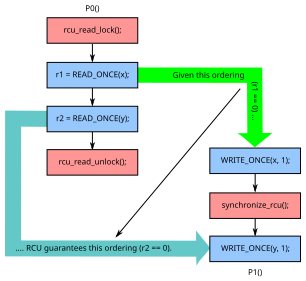
\includegraphics{defer/RCUGuaranteeFwd}}
\caption{RCU Reader and Later Grace Period}
\label{fig:defer:RCU Reader and Later Grace Period}
\end{figure}

The relationship between an RCU read-side critical section and a later
RCU grace period is an if-then relationship, as illustrated by
\cref{fig:defer:RCU Reader and Later Grace Period}.
If any portion of a given critical section precedes the beginning of
a given grace period, then RCU guarantees that all of that critical
section will precede the end of that grace period.
However, RCU users cannot directly determine the order in which these
\co{rcu_read_lock()} and \co{synchronize_rcu()} invocations are executed,
but must instead deduce the order based on the behavior of nearby memory
references.
The filled green arrow at the top of the figure indicates that \co{P0()}'s
\co{READ_ONCE()} from \co{x} returns zero, that is, the value overwritten
by \co{P1()}'s \co{WRITE_ONCE()} to this same variable.
This in turn implies that \co{P0()}'s \co{rcu_read_lock()} must have
executed before \co{P1()}'s \co{WRITE_ONCE()} to \co{x} and thus before
its call to \co{synchronize_rcu()}, which therefore cannot return until
after \co{P0()} executes its \co{rcu_read_unlock()}.
And finally, the black arrow leading from the filled green arrow
to the filled blue arrow indicates that \co{P0()}'s \co{READ_ONCE()}
from \co{y} must happen before \co{P1()}'s \co{WRITE_ONCE()} to \co{y},
thus guaranteeing that \co{r2}'s final value will be zero.

\QuickQuiz{
	What other final values of \co{r1} and \co{r2} are possible in
	\cref{fig:defer:RCU Reader and Later Grace Period}?
}\QuickQuizAnswer{
	The \co{r1 == 0 && r2 == 0} possibility was called out in the text.
	Given that \co{r1 == 0} implies \co{r2 == 0}, we know that
	\co{r1 == 0 && r2 == 1} is forbidden.
	The following discussion will show that both
	\co{r1 == 1 && r2 == 1} and \co{r1 == 1 && r2 == 0} are possible.
}\QuickQuizEnd

\begin{figure}
\centering
\resizebox{3in}{!}{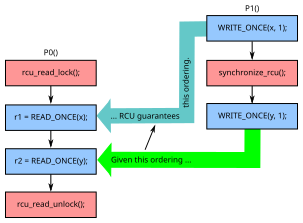
\includegraphics{defer/RCUGuaranteeRev}}
\caption{RCU Reader and Earlier Grace Period}
\label{fig:defer:RCU Reader and Earlier Grace Period}
\end{figure}

But suppose that the \co{rcu_read_unlock()} ending a given task's RCU
read-side critical section is executed after the return from a second
task's call to \co{synchronize_rcu()}.
Because \co{synchronize_rcu()} cannot return until all task have
exited any pre-existing RCU read-side critical sections, it must be the
case that the second task called \co{synchronize_rcu()} before first
task executed the matching \co{rcu_read_lock()}.
This means that this call to \co{synchronize_rcu()} must happen before
the entirety of the first task's RCU read-side critical section,
although the actual execution of \co{synchronize_rcu()} might well
overlap with the critical section.

This constraint is illustrated by
\cref{fig:defer:RCU Reader and Earlier Grace Period},
with the call to \co{synchronize_rcu()} represented by \co{P1()}'s
topmost arrow and the corresponding return by its bottommost arrow.
Again, RCU users cannot directly determine the order in which these
\co{rcu_read_unlock()} and \co{synchronize_rcu()} invocations are executed,
but must instead deduce the order based on the behavior of nearby memory
references.
The lower filled green arrow indicates that \co{P0()}'s \co{READ_ONCE()}
from \co{y} returned the value~1 and thus happened after \co{P1()}'s
\co{WRITE_ONCE()} to \co{y}, but it also indicates that \co{P0()}'s
call to \co{rcu_read_unlock()} followed the return from \co{P1()}'s call
to \co{synchronize_rcu()}.
Therefore, as indicated by the black arrow leading from the filled green
arrow to the filled blue arrow, \co{P0()}'s \co{READ_ONCE()} from \co{x}
must follow \co{P1()}'s \co{WRITE_ONCE()} to \co{x}, thus guaranteeing
that if \co{r2}'s final value is~1, then \co{r1}'s final value must
also be~1.

\QuickQuiz{
	What would happen if the order of \co{P0()}'s two accesses was
	reversed in
	\cref{fig:defer:RCU Reader and Earlier Grace Period}?
}\QuickQuizAnswer{
	Absolutely nothing would change.
	The fact that \co{P0()}'s loads from \co{x} and \co{y} are
	in the same RCU read-side critical section suffices;
	their order is irrelevant.
}\QuickQuizEnd

\begin{figure}
\centering
\resizebox{3in}{!}{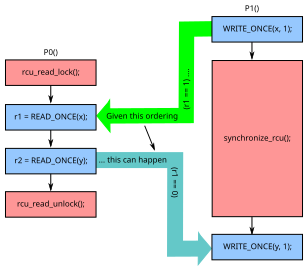
\includegraphics{defer/RCUGuaranteeMid}}
\caption{RCU Reader Within Grace Period}
\label{fig:defer:RCU Reader Within Grace Period}
\end{figure}

Finally, as shown in
\cref{fig:defer:RCU Reader Within Grace Period},
an RCU read-side critical section can be completely overlapped by
an RCU grace period.
Because \co{P0()}'s \co{rcu_read_lock()} executed after \co{P1()}'s
call to \co{synchronize_rcu()}, the return from that call need not
wait for \co{P0()}'s \co{rcu_read_unlock()}.
Furthermore, \co{rcu_read_unlock()} need never wait on anything at all.
Therefore, \co{r1}'s final value is 1 and \co{r2}'s final value is 0.
The key point is that \co{P0()}'s RCU read-side critical section is in
no way obligated to wait on \co{P1()}'s grace period.

However, it cannot be the case that \co{r1}'s final value is 0 and \co{r2}'s
final value is 1.
This would mean that an RCU read-side critical section had completely
overlapped a grace period, which is forbidden (or at the very least
constitutes a bug in RCU)\@.
RCU's wait-for-readers guarantee therefore has two parts:
\begin{enumerate*}[(1)]
\item If any part of a given RCU read-side critical section precedes
the beginning of a given grace period, then the entirety of that
critical section precedes the end of that grace period.
\item If any part of a given RCU read-side critical section follows
the end of a given grace period, then the entirety of that
critical section follows the beginning of that grace period.
\end{enumerate*}
This definition is sufficient for almost all RCU-based algorithms, but
for those wanting more,
simple executable formal models of RCU are available
as part of Linux kernel v4.17 and later, as discussed in
\cref{sec:formal:Axiomatic Approaches and RCU}.
In addition, RCU's ordering properties are examined in much
greater detail in \cref{sec:memorder:RCU}.

\QuickQuiz{
	What would happen if \co{P0()}'s accesses in
	\crefrange{fig:defer:RCU Reader and Later Grace Period}{fig:defer:RCU Reader Within Grace Period}
	were stores?
}\QuickQuizAnswer{
	The exact same ordering rules would apply, that is,
	(1)~If any part of \co{P0()}'s RCU read-side critical section
	preceded the beginning of \co{P1()}'s grace period, all of
	\co{P0()}'s RCU read-side critical section would precede the
	end of \co{P1()}'s grace period, and
	(2)~If any part of \co{P0()}'s RCU read-side critical section
	followed the end of \co{P1()}'s grace period, all of \co{P0()}'s
	RCU read-side critical section would follow the beginning of
	\co{P1()}'s grace period.
	The only difference is that the RCU user would look not at
	some value loaded via \co{READ_ONCE()} but instead at the final
	values of the written-to variables.

	It might seem strange to have RCU read-side critical sections
	containing writes, but this capability is not only permitted,
	but also highly useful.
	For example, the Linux kernel frequently carries out an
	RCU-protected traversal of a linked data structure and then
	acquires a reference to the destination data element.
	Because this data element must not be freed in the meantime,
	that element's reference counter must necessarily be incremented
	within the traversal's RCU read-side critical section.
	However, that increment entails a write to memory.
	Therefore, it is a very good thing that memory writes are
	permitted within RCU read-side critical sections.

	If having writes in RCU read-side critical sections still seems
	strange, please review
	\cref{sec:count:Applying Exact Limit Counters},
	which presented a use case for writes in reader-writer locking
	read-side critical sections.
}\QuickQuizEnd

Although RCU's wait-for-readers capability really is sometimes used to
order the assignment of values to variables as shown in
\crefrange{fig:defer:RCU Reader and Later Grace Period}
{fig:defer:RCU Reader Within Grace Period},
it is more frequently used to safely free data elements removed from
a linked structure, as was done in
\cref{sec:defer:Introduction to RCU}.
The general process is illustrated by the following pseudocode:

\begin{enumerate}
\item	Make a change, for example, remove an element from a linked list.
\item	Wait for all pre-existing RCU read-side critical sections to
	completely finish (for example, by invoking
	\co{synchronize_rcu()}).
\item	Clean up, for example, free the element that was replaced above.
\end{enumerate}

\begin{figure}
\centering
\IfEbookSize{
\resizebox{2in}{!}{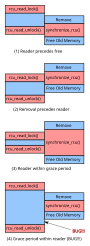
\includegraphics{defer/RCUGPorderingSummary}}
}{
\resizebox{2.5in}{!}{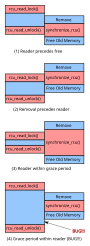
\includegraphics{defer/RCUGPorderingSummary}}
}
\caption{Summary of RCU Grace-Period Ordering Guarantees}
\label{fig:defer:Summary of RCU Grace-Period Ordering Guarantees}
\end{figure}

This more abstract procedure requires a more abstract diagram than
\crefrange{fig:defer:RCU Reader and Later Grace Period}
{fig:defer:RCU Reader Within Grace Period},
which are specific to a particular litmus test.
After all, an RCU implementation must work correctly regardless of
the form of the RCU updates and the RCU read-side critical sections.
\Cref{fig:defer:Summary of RCU Grace-Period Ordering Guarantees}
fills this need, showing the four possible scenarios, with time
advancing from top to bottom within each scenario.
Within each scenario, an RCU reader is represented by the left-hand
stack of boxes and RCU updater by the right-hand stack.

In the first scenario, the reader starts execution before the
updater starts the removal, so it is possible that this reader
has a reference to the removed data element.
Therefore, the updater must not free this element until after the
reader completes.
In the second scenario, the reader does not start execution until
after the removal has completed.
The reader cannot possibly obtain a reference to the already-removed
data element, so this element may be freed before the reader completes.
The third scenario is like the second, but illustrates that even when the
reader cannot possibly obtain a reference to an element, it is still
permissible to defer the freeing of that element until after the
reader completes.
In the fourth and final scenario, the reader starts execution before
the updater starts removing the data element, but this element
is (incorrectly) freed before the reader completed.
A correct RCU implementation will not allow this fourth scenario to
occur.
This diagram thus illustrates RCU's wait-for-readers functionality:
Given a grace period, each reader ends before the end of that grace
period, starts after the beginning of that grace period, or both, in
which case it is wholly contained within that grace period.

Because RCU readers can make forward progress while updates
are in progress, different readers might disagree about the state
of the data structure, a topic taken up by the next section.

\subsubsection{Maintain Multiple Versions of Recently Updated Objects}
\label{sec:defer:Maintain Multiple Versions of Recently Updated Objects}

This section discusses how RCU accommodates synchronization-free readers
by maintaining multiple versions of data.
Because these synchronization-free readers provide very weak temporal
synchronization, RCU users compensate via spatial synchronization.
Spatial synchronization was discussed in
\cref{chp:Partitioning and Synchronization Design}, and is heavily used
in practice to obtain good performance and scalability.
In this section, spatial synchronization will be used to attain a weak
(but useful) form of correctness as well as excellent performance and
scalability.

\Cref{fig:defer:Deletion With Concurrent Readers}
in
\cref{sec:defer:Minimal Insertion and Deletion}
showed a simple variant of spatial synchronization, in which different
readers running concurrently with \co{del_route()}
(see \cref{lst:defer:Insertion and Deletion With Concurrent Readers})
might see the old \co{route} structure or an empty list, but either
way get a valid result.
Of course, a closer look at
\cref{fig:defer:Insertion With Concurrent Readers}
shows that calls to \co{ins_route()} can also result in concurrent
readers seeing different versions:
Either the initial empty list or the newly inserted \co{route} structure.
Note that both reference counting
(\cref{sec:defer:Reference Counting})
and hazard pointers
(\cref{sec:defer:Hazard Pointers})
can also cause concurrent readers to see different versions, but
RCU's lightweight readers make this more likely.

\begin{figure}
\centering
\resizebox{3in}{!}{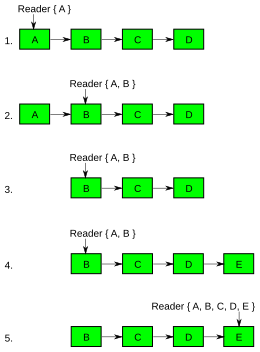
\includegraphics{defer/multver}}
\caption{Multiple RCU Data-Structure Versions}
\label{fig:defer:Multiple RCU Data-Structure Versions}
\end{figure}

However, maintaining multiple weakly consistent versions can provide
some surprises.
For example, consider
\cref{fig:defer:Multiple RCU Data-Structure Versions},
in which a reader is traversing a linked list that is concurrently
updated.\footnote{
	RCU linked-list APIs may be found in
	\cref{sec:defer:RCU Linux-Kernel API}.}
In the first row of the figure, the reader is referencing data item~A,
and in the second row, it advances to~B, having thus far seen A followed by~B\@.
In the third row, an updater removes element~A and in the fourth row
an updater adds element~E to the end of the list.
In the fifth and final row, the reader completes its traversal, having
seeing elements~A through~E\@.

Except that there was no time at which such a list existed.
This situation might be even more surprising than that shown in
\cref{fig:defer:Deletion With Concurrent Readers},
in which different concurrent readers see different versions.
In contrast, in
\cref{fig:defer:Multiple RCU Data-Structure Versions}
the reader sees a version that never actually existed!

One way to resolve this strange situation is via weaker semantics.
A reader traversal must encounter any data item that was present
during the full traversal (B, C, and~D), and might or might not
encounter data items that were present for only part of the
traversal (A and~E)\@.
Therefore, in this particular case, it is perfectly legitimate for
the reader traversal to encounter all five elements.
If this outcome is problematic, another way to resolve this situation is
through use of stronger synchronization mechanisms, such as reader-writer
locking, or clever use of timestamps and versioning,
as discussed in \cref{sec:defer:Quasi Multi-Version Concurrency Control}.
Of course, stronger mechanisms will be more expensive, but then again
the engineering life is all about choices and tradeoffs.

Strange though this situation might seem, it is entirely consistent with
the real world.
As we saw in
\cref{sec:cpu:Overheads},
the finite speed of light cannot be ignored within a computer system,
and it most certainly cannot be ignored outside of this system.
This in turn means that any data within the system representing state
in the real world outside of the system is always and forever outdated,
and thus inconsistent with the real world.
Therefore, it is quite possible that the sequence \{A, B, C, D, E\}
occurred in the real world, but due to speed-of-light delays was
never represented in the computer system's memory.
In this case, the reader's surprising traversal would correctly reflect
reality.

As a result, algorithms operating on real-world data must account for
inconsistent data, either by tolerating inconsistencies or by taking
steps to exclude or reject them.
In many cases, these algorithms are also perfectly capable of dealing
with inconsistencies within the system.

The pre-BSD packet routing example laid out in
\cref{sec:defer:Running Example}
is a case in point.
The contents of a routing list is set by routing protocols, and these
protocols feature significant delays (seconds or even minutes) to avoid
routing instabilities.
Therefore, once a routing update reaches a given system,
it might well have been sending packets the wrong way for quite some time.
Sending a few more packets the wrong way for the few microseconds during
which the update is in flight is clearly not a problem because the same
higher-level protocol actions that deal with delayed routing updates
will also deal with internal inconsistencies.

Nor is Internet routing the only situation tolerating inconsistencies.
To repeat, any algorithm in which data within a system tracks
outside-of-system state must tolerate inconsistencies, which includes
security policies (often set by committees of humans), storage configuration,
and WiFi access points, to say nothing of removable hardware such as
microphones, headsets, cameras, mice, printers, and much else besides.
Furthermore, the large number of Linux-kernel RCU API uses shown in
\cref{fig:defer:RCU Usage in the Linux Kernel},
combined with the Linux kernel's heavy use of reference counting
and with increasing use of \IXpl{hazard pointer} in other projects, demonstrates
that tolerance for such inconsistencies is more common than one might
imagine.

One root cause of this common-case tolerance of inconsistencies is
that single-item lookups are much more common in practice than are
full-data-structure traversals.
After all, full-data-structure traversals are much more expensive than
single-item lookups, so developers are motivated to avoid such traversals.
Not only are concurrent updates less likely to affect a single-item
lookup than they are a full traversal, but it is also the case that an
isolated single-item lookup has no way of detecting such inconsistencies.
As a result, in the common case, such inconsistencies are not just
tolerable, they are in fact invisible.

In such cases, RCU readers can be considered to be fully ordered with
updaters, despite the fact that these readers might be executing the
exact same sequence of machine instructions that would be executed by
a single-threaded program, as hinted on
\cpageref{sec:defer:Mysteries RCU}.
For example, referring back to
\cref{lst:defer:Insertion and Deletion With Concurrent Readers}
on \cpageref{lst:defer:Insertion and Deletion With Concurrent Readers},
suppose that each reader thread invokes \co{access_route()} exactly
once during its lifetime, and that there is no other communication among
reader and updater threads.
\begin{fcvref}[ln:defer:Insertion and Deletion With Concurrent Readers]
Then each invocation of \co{access_route()} can be ordered after the
\co{ins_route()} invocation that produced the \co{route} structure
accessed by \clnref{access_rp} of the listing in \co{access_route()}
and ordered before any subsequent
\co{ins_route()} or \co{del_route()} invocation.
\end{fcvref}

In summary, maintaining multiple versions is exactly what enables the
extremely low overheads of RCU readers, and as noted earlier, many
algorithms are unfazed by multiple versions.
However, there are algorithms that absolutely cannot handle multiple versions.
There are techniques for adapting such algorithms to
RCU~\cite{PaulEdwardMcKenneyPhD}, for example, the use of sequence locking
described in \cref{sec:together:Correlated Data Elements}.

\paragraph{Exercises}
\label{sec:defer:Exercises}

These examples assumed that a mutex was held across the entire
update operation, which would mean that there could be at most two
versions of the list active at a given time.

\QuickQuizSeries{%
\QuickQuizB{
	How would you modify the deletion example to permit more than two
	versions of the list to be active?
}\QuickQuizAnswerB{
	One way of accomplishing this is as shown in
	\cref{lst:defer:Concurrent RCU Deletion}.

\begin{listing}
\begin{VerbatimL}
spin_lock(&mylock);
p = search(head, key);
if (p == NULL)
	spin_unlock(&mylock);
else {
	list_del_rcu(&p->list);
	spin_unlock(&mylock);
	synchronize_rcu();
	kfree(p);
}
\end{VerbatimL}
\caption{Concurrent RCU Deletion}
\label{lst:defer:Concurrent RCU Deletion}
\end{listing}

	Note that this means that multiple concurrent deletions might be
	waiting in \co{synchronize_rcu()}.
}\QuickQuizEndB
%
\QuickQuizM{
	How many RCU versions of a given list can be
	active at any given time?
}\QuickQuizAnswerM{
	That depends on the synchronization design.
	If a semaphore protecting the update is held across the grace period,
	then there can be at most two versions, the old and the new.

	However, suppose that only the search, the update, and the
	\co{list_replace_rcu()} were protected by a lock, so that
	the \co{synchronize_rcu()} was outside of that lock, similar
	to the code shown in
	\cref{lst:defer:Concurrent RCU Deletion}.
	Suppose further that a large number of threads undertook an
	RCU replacement at about the same time, and that readers
	are also constantly traversing the data structure.

	Then the following sequence of events could occur, starting from
	the end state of
	\cref{fig:defer:Multiple RCU Data-Structure Versions}:

	\begin{enumerate}
	\item	Thread~A traverses the list, obtaining a reference to
		Element~C.
	\item	Thread~B replaces Element~C with a new
		Element~F, then waits for its \co{synchronize_rcu()}
		call to return.
	\item	Thread~C traverses the list, obtaining a reference to
		Element~F.
	\item	Thread~D replaces Element~F with a new
		Element~G, then waits for its \co{synchronize_rcu()}
		call to return.
	\item	Thread~E traverses the list, obtaining a reference to
		Element~G.
	\item	Thread~F replaces Element~G with a new
		Element~H, then waits for its \co{synchronize_rcu()}
		call to return.
	\item	Thread~G traverses the list, obtaining a reference to
		Element~H.
	\item	And the previous two steps repeat quickly with additional
		new elements, so that all of them happen before any of
		the \co{synchronize_rcu()} calls return.
	\end{enumerate}

	Thus, there can be an arbitrary number of versions active,
	limited only by memory and by how many updates could be completed
	within a grace period.
	But please note that data structures that are updated so frequently
	are not likely to be good candidates for RCU\@.
	Nevertheless, RCU can handle high update rates when necessary.
}\QuickQuizEndM
%
\QuickQuizE{
	How can the per-update overhead of RCU be reduced?
}\QuickQuizAnswerE{
	The most effective way to reduce the per-update overhead
	of RCU is to increase the number of updates served by
	a given grace period.
	This works because the per-grace period overhead is nearly
	independent of the number of updates served by that
	grace period.

	One way to do this is to delay the start of a given grace
	period in the hope that more updates requiring that grace
	period appear in the meantime.
	Another way is to slow down execution of the grace period
	in the hope that more updates requiring an additional
	grace period will accumulate in the meantime.

	There are many other possible optimizations, and fanatically
	devoted readers are referred to the Linux-kernel RCU
	implementation.
}\QuickQuizEndE
}

\subsubsection{Summary of RCU Fundamentals}
\label{sec:defer:Summary of RCU Fundamentals}

This section has described the three fundamental components of RCU-based
linked-structure algorithms:

\begin{enumerate}
\item	A publish-subscribe mechanism for adding new data featuring
	\co{rcu_assign_pointer()} for update-side publication and
	\co{rcu_dereference()} for read-side subscription,

\item	A way of waiting for pre-existing RCU readers to finish
	based on readers being delimited by \co{rcu_read_lock()}
	and \co{rcu_read_unlock()} on the one hand and
	updaters waiting via \co{synchronize_rcu()} or
	\co{call_rcu()} on the other
	(see \cref{sec:memorder:RCU} for a formal description),
	and

\item	A discipline of maintaining multiple versions to permit
	change without harming or unduly delaying concurrent RCU readers.
\end{enumerate}

\QuickQuiz{
	How can RCU updaters possibly delay RCU readers, given that
	neither \co{rcu_read_lock()} nor \co{rcu_read_unlock()}
	spin or block?
}\QuickQuizAnswer{
	The modifications undertaken by a given RCU updater will cause the
	corresponding CPU to invalidate cache lines containing the data,
	forcing the CPUs running concurrent RCU readers to incur expensive
	cache misses.
	(Can you design an algorithm that changes a data structure
	\emph{without}
	inflicting expensive cache misses on concurrent readers?
	On subsequent readers?)
}\QuickQuizEnd

These three RCU components allow data to be updated in the face of concurrent
readers that might be executing the same sequence of machine instructions
that would be used by a reader in a single-threaded implementation.
These RCU components can be combined in different ways to implement a
surprising variety of different types of RCU-based algorithms, a number
of which are presented in
\cref{sec:defer:RCU Usage}.
However, it is usually better to work at higher levels of abstraction.
To this end, the next section describes the Linux-kernel API, which
includes simple data structures such as lists.

% defer/rcuAPI.tex
% mainfile: ../perfbook.tex
% SPDX-License-Identifier: CC-BY-SA-3.0

\subsection{RCU Linux-Kernel API}
\label{sec:defer:RCU Linux-Kernel API}
\OriginallyPublished{sec:defer:RCU Linux-Kernel API}{RCU Linux-Kernel API}{Linux Weekly News}{PaulEMcKenney2008WhatIsRCUAPI}

This section looks at RCU from the viewpoint of its Linux-kernel API\@.\footnote{
	Userspace RCU's API is documented
	elsewhere~\cite{PaulMcKenney2013LWNURCU}.}
\Cref{sec:defer:RCU API and Software Engineering}
explores the relationship between RCU's API and software engineering,
\cref{sec:defer:RCU has a Family of Wait-to-Finish APIs}
presents RCU's wait-to-finish APIs,
\cref{sec:defer:RCU has Publish-Subscribe and Version-Maintenance APIs}
presents RCU's publish-subscribe and version-maintenance APIs,
\cref{sec:defer:RCU has List-Processing APIs}
presents RCU's list-processing APIs,
\cref{sec:defer:RCU Has Diagnostic APIs}
presents RCU's diagnostic APIs, and
\cref{sec:defer:Where Can RCU's APIs Be Used?}
describes in which contexts RCU's various APIs may be used.
Finally,
\cref{sec:defer:So; What is RCU Really?}
presents concluding remarks.

Readers who are not excited about kernel internals may wish to skip
ahead to \cref{sec:defer:RCU Usage}
on \cpageref{sec:defer:RCU Usage},
but preferably after reviewing the next section covering software-engineering
considerations.

\subsubsection{RCU API and Software Engineering}
\label{sec:defer:RCU API and Software Engineering}

Readers who have looked ahead to
\cref{tab:defer:RCU Wait-to-Finish APIs,%
tab:defer:RCU Markers for Read-Side Critical Sections,%
tab:defer:SRCU Markers for Read-Side Critical Sections,%
tab:defer:RCU Polled Update-Side Primitives,%
tab:defer:RCU Publish-Subscribe and Version Maintenance APIs,%
tab:defer:RCU-Protected List APIs,%
tab:defer:RCU Diagnostic APIs}
might have noted that the full list of Linux-kernel APIs sports more
than 100 members.
This is in sharp (and perhaps dismaying) contrast to the mere six
API members shown in
\cref{tab:defer:Core RCU API}.
This situation clearly raises the question ``Why so many???''

This question is answered more thoroughly in the following sections,
but in the meantime the rest of this section summarizes the motivations.

There is a wise old saying to the effect of ``To err is human.''
This means that the purpose of a significant fraction of the RCU API is to
provide diagnostics, most notably in \cref{tab:defer:RCU Diagnostic APIs},
but elsewhere as well.

Important causes of human error are the limits of the human brain,
for example, the limited capacity of short-term memory.
The toy examples shown in this book do not stress these limits.
This is out of necessity:
Many readers push their cognitive limits while learning new material,
so the examples need to be kept simple.

These examples therefore keep \co{rcu_dereference()} invocations
in the same function as the enclosing \co{rcu_read_lock()} and
\co{rcu_read_unlock()} calls.
In contrast, real-world software must frequently invoke these API members
from different functions, and even from different translation units.
The Linux kernel RCU API has therefore expanded to accommodate lockdep,
which allows \co{rcu_dereference()} and friends to complain if it is
not protected by \co{rcu_read_lock()}.
Linux-kernel RCU also checks for some double-free errors, infinite
loops in RCU read-side critical sections, and attempts to invoke
quiescent states within RCU read-side critical sections.

Another way that real-world software accommodates the limits of human
cognition is through abstraction.
The Linux-kernel API therefore includes members that operate on lists
in addition to the pointer-oriented core API of
\cref{tab:defer:Core RCU API}.
The Linux kernel itself also provides RCU-protected hash tables and
search trees.

Operating-systems kernels such as Linux operate near the bottom of the
``iron triangle'' of the software stack shown in
\cref{fig:intro:Software Layers and Performance; Productivity; and Generality},
where performance is critically important.
There are thus specialized variants of a number of RCU APIs for use on
fastpaths, for example, as discussed in
\cref{sec:defer:RCU has Publish-Subscribe and Version-Maintenance APIs},
\co{RCU_INIT_POINTER()} may be used in
place of \co{rcu_assign_pointer()} in cases where the RCU-protected pointer
is being assigned to \co{NULL} or when that pointer is not yet accessible
by readers.
Use of \co{RCU_INIT_POINTER()} allows the compiler more leeway in
selecting instructions and carrying out optimizations, thus increasing
performance.

On the other hand, when used incorrectly \co{RCU_INIT_POINTER()} can
result in silent memory corruption, so please be careful!
Yes, in some cases, the kernel can check for inappropriate use of
RCU API members from a given kernel context, but the constraints of
\co{RCU_INIT_POINTER()} use are not yet checkable.

Finally, within the Linux kernel, the aforementioned limits of human
cognition are compounded by the variety and severity of workloads running
on Linux.
As of v5.16, this has given rise to no fewer than five flavors of
RCU, each designed to provide different performance, scalability,
response-time, and energy efficiency tradeoffs to RCU readers and writers.
These RCU flavors are the subject of the next section.

\subsubsection{RCU has a Family of Wait-to-Finish APIs}
\label{sec:defer:RCU has a Family of Wait-to-Finish APIs}

The most straightforward answer to ``what is RCU'' is that RCU is
an API\@.
For example, the RCU implementation used in the Linux kernel is
summarized by
\cref{tab:defer:RCU Wait-to-Finish APIs},
whose columns show the wait-for-readers portions of the RCU, ``sleepable''
RCU (SRCU), Tasks RCU, Tasks RCU Rude, Tasks RCU Trace, and generic APIs,
respectively,
\cref{tab:defer:RCU Markers for Read-Side Critical Sections},
which shows the full range of RCU read-side markers,
\cref{tab:defer:SRCU Markers for Read-Side Critical Sections},
which shows the full range of SRCU read-side markers,
\cref{tab:defer:RCU Polled Update-Side Primitives},
which shows the full RCU polled grace-period API,
and by
\cref{tab:defer:RCU Publish-Subscribe and Version Maintenance APIs},
which shows the publish-subscribe portions of the
API~\cite{PaulEMcKenney2024RCUAPI}.\footnote{
	This citation covers v6.10 and later.
	Documentation for earlier versions of the Linux-kernel RCU API may
	be found elsewhere~\cite{PaulEMcKenney2008WhatIsRCUAPI,PaulEMcKenney2014RCUAPI,PaulEMcKenney2019RCUAPI}.}

\begin{sidewaystable*}[tbp]
\rowcolors{1}{}{lightgray}
\renewcommand*{\arraystretch}{1.3}
\centering
\caption{RCU Wait-to-Finish APIs}
\label{tab:defer:RCU Wait-to-Finish APIs}
\scriptsize\IfEbookSize{\hspace*{-1.8in}}{\hspace*{-.125in}}
\ebresizeverb{0.7}{
\begin{tabularx}{8.5in}{>{\raggedright\arraybackslash}p{0.92in}
    >{\raggedright\arraybackslash}p{1.37in}
    >{\raggedright\arraybackslash}p{1.39in}
    >{\raggedright\arraybackslash}p{1.09in}
    >{\raggedright\arraybackslash}p{1.34in}
    >{\raggedright\arraybackslash}p{1.44in}}
\toprule
&
    {\bf RCU}: Original &
	{\bf SRCU}: Sleeping readers &
	    {\bf Tasks RCU}: Free tracing trampolines &
		{\bf Tasks RCU Rude}: Free idle-task tracing trampolines &
		    {\bf Tasks RCU Trace}: Protect sleepable BPF programs \\
\midrule
{\bf Initialization and Cleanup} &
    &
	\tco{DEFINE_SRCU()} \tco{DEFINE_STATIC_SRCU()}
	\tco{init_srcu_struct()} \tco{cleanup_srcu_struct()} &
	    &
		&
		    \\
{\bf Read-side critical-section markers} &
    \tco{rcu_read_lock()}~! \tco{rcu_read_unlock()}~!  ~~~~~~~~~~~~~~~~~~
    (See \cref{tab:defer:RCU Markers for Read-Side Critical Sections} for more.) &
	\tco{srcu_read_lock()} \tco{srcu_read_unlock()} ~~~~~~~~~~~~~~~~~
	(See \cref{tab:defer:SRCU Markers for Read-Side Critical Sections} for more.) &
	    Voluntary context switch in non-idle tasks. &
		Preemption-disabled regions of code. &
		    \tco{rcu_read_lock_trace()} \tco{rcu_read_unlock_trace()}
		    \tco{guard(rcu_tasks_trace)()}
		    \tco{scoped_guard(rcu_tasks_trace)} \\
{\bf Update-side primitives (synchronous) } &
    { \tco{synchronize_rcu()}
      \tco{synchronize_net()}
      \tco{synchronize_rcu_expedited()} } &
	\tco{synchronize_srcu()} \tco{synchronize_srcu_expedited()} &
	    \tco{synchronize_rcu_tasks()}
	    \tco{synchronize_rcu_mult()} &
		\tco{synchronize_rcu_tasks_rude()} &
		    \tco{synchronize_rcu_tasks_trace()}
		    \tco{rcu_trace_implies_rcu_gp()} \\
{\bf Update-side primitives (asynchronous / callback) } &
    \tco{call_rcu()} ! ~~~~~~
    \tco{call_rcu_hurry()} &
	\tco{call_srcu()} &
	    \tco{call_rcu_tasks()} &
		\tco{call_rcu_tasks_rude()} &
		    \tco{call_rcu_tasks_trace()} \\
{\bf Update-side primitives (wait for callbacks) } &
    \tco{rcu_barrier()} &
	\tco{srcu_barrier()} &
	    \tco{rcu_barrier_tasks()} &
		\tco{rcu_barrier_tasks_rude()} &
		    \tco{rcu_barrier_tasks_trace()} \\
{\bf Update-side primitives (polled) } &
    \tco{get_state_synchronize_rcu()}
    \tco{start_poll_synchronize_rcu()}
    \tco{poll_state_synchronize_rcu()} ~~~~~~~~~~~~~~~~~~
    (See \cref{tab:defer:RCU Polled Update-Side Primitives} for more.) &
	\tco{get_state_synchronize_srcu()}
	\tco{start_poll_synchronize_srcu()}
	\tco{poll_state_synchronize_srcu()} &
	    &
		&
		    \\
{\bf Update-side primitives (initiate / wait)} &
    \tco{get_state_synchronize_rcu()}
    \tco{cond_synchronize_rcu()} &
	&
	    &
		&
		    \\
{\bf Update-side primitives (free memory) } &
    \tco{kfree_rcu()}
    \tco{kfree_rcu_mightsleep()}
    \tco{kvfree_rcu()}
    \tco{kvfree_rcu_mightsleep()} &
	&
	    &
		&
		    \\
{\bf Type-safe memory } &
    \tco{SLAB_TYPESAFE_BY_RCU} &
	&
	    &
		&
		    \\
{\bf Read side constraints } &
    No blocking (only preemption) &
	No \tco{synchronize_srcu()} with same \tco{srcu_struct} &
	    No voluntary context switch &
		Neither blocking nor preemption &
			No RCU tasks trace grace period \\
{\bf Read side overhead } &
    CPU-local accesses (\tco{barrier()} on \tco{PREEMPT=n}) &
	Simple instructions, memory barriers &
	    Free &
		CPU-local accesses (free on \tco{PREEMPT=n}) &
		    CPU-local accesses \\
{\bf Asynchronous update-side overhead } &
    sub-microsecond &
	sub-microsecond &
	    sub-microsecond &
		sub-microsecond &
		    sub-microsecond \\
{\bf Grace-period latency } &
    10s of milliseconds &
        Milliseconds &
	    Seconds &
		Milliseconds &
		    10s of milliseconds \\
{\bf Expedited grace-period latency } &
    10s of microseconds &
        Microseconds &
	    N/A &
		N/A &
		    N/A \\
\bottomrule
\end{tabularx}
}
\end{sidewaystable*}

\begin{table*}
\rowcolors{1}{}{lightgray}
\renewcommand*{\arraystretch}{1.15}
\footnotesize
\centering\OneColumnHSpace{-.4in}
\ebresizewidth{
\begin{tabular}{llp{2.0in}}
\toprule
Acquisition &
	Release &
		Comments \\
\midrule
\tco{rcu_read_lock()} &
	\tco{rcu_read_unlock()} & \\
\tco{guard(rcu)()} & & RCU reader to end of enclosing scope. \\
\tco{scoped_guard(rcu)} & & RCU reader for following statement. \\
\tco{rcu_read_lock_bh()} &
	\tco{rcu_read_unlock_bh()} & \\
\tco{rcu_read_lock_sched()} &
	\tco{rcu_read_unlock_sched()} & \\
\tco{rcu_read_lock_sched_notrace()} &
	\tco{rcu_read_unlock_sched_notrace()} & \\
\tco{local_bh_disable()} &
	\tco{local_bh_enable()} &
		And anything else that disables bottom halves. \\
\tco{preempt_disable()} &
	\tco{preempt_enable()} &
		And anything else that disables preemption. \\
\tco{local_irq_save()} &
	\tco{local_irq_restore()} &
		And anything else that disables interrupts. \\
\bottomrule
\end{tabular}
}
\caption{RCU Markers for Read-Side Critical Sections}
\label{tab:defer:RCU Markers for Read-Side Critical Sections}
\end{table*}

\begin{table*}
\rowcolors{1}{}{lightgray}
\renewcommand*{\arraystretch}{1.15}
\footnotesize
\centering\OneColumnHSpace{-.4in}
\ebresizewidth{
\begin{tabular}{llp{2.0in}}
\toprule
Acquisition &
	Release &
		Comments \\
\midrule
\tco{srcu_read_lock()} &
	\tco{srcu_read_unlock()} & \\
\tco{guard(srcu)(&my_srcu)} & & SRCU reader to end of enclosing scope. \\
\tco{scoped_guard(srcu, &my_srcu)} & & SRCU reader for following statement. \\
\tco{srcu_read_lock_nmisafe()} &
	\tco{srcu_read_unlock_nmisafe()} & \\
\tco{srcu_read_lock_notrace()} &
	\tco{srcu_read_unlock_notrace()} & \\
\tco{srcu_down_read()} &
	\tco{srcu_up_read()} & \\
\bottomrule
\end{tabular}
}
\caption{SRCU Markers for Read-Side Critical Sections}
\label{tab:defer:SRCU Markers for Read-Side Critical Sections}
\end{table*}

\begin{table*}
\rowcolors{1}{}{lightgray}
\renewcommand*{\arraystretch}{1.15}
\footnotesize
\centering\OneColumnHSpace{-.4in}
\ebresizewidth{
\begin{tabular}{p{2.5in}p{2.5in}}
\toprule
Compressed State / Full State &
		Comments \\
\midrule
\tco{get_completed_synchronize_rcu()}
\tco{get_completed_synchronize_rcu_full()} &
	Return always-completed state. \\
\tco{get_state_synchronize_rcu()}
\tco{get_state_synchronize_rcu_full()} &
	Return state for grace-period completion. \\
\tco{start_poll_synchronize_rcu()}
\tco{start_poll_synchronize_rcu_full()} &
	Return state for grace-period completion and start
	a grace period if needed. \\
\tco{start_poll_synchronize_rcu_expedited()}
\tco{start_poll_synchronize_rcu_expedited_full()} &
	Return state for grace-period completion and start
	an expedited grace period if needed. \\
\tco{poll_state_synchronize_rcu()}
\tco{poll_state_synchronize_rcu_full()} &
	Return true if state's grace period has ended. \\
\tco{cond_synchronize_rcu()}
\tco{cond_synchronize_rcu_full()} &
	Wait (if needed) for state's grace period to end. \\
\tco{cond_synchronize_rcu_expedited()}
\tco{cond_synchronize_rcu_expedited_full()} &
	Expedited wait (if needed) for state's grace period to end. \\
\tco{NUM_ACTIVE_RCU_POLL_OLDSTATE}
\tco{NUM_ACTIVE_RCU_POLL_OLDSTATE_FULL} &
	Maximum number of states corresponding to in-flight grace
	periods. \\
\tco{same_state_synchronize_rcu()}
\tco{same_state_synchronize_rcu_full()} &
	Are two states equivalent? \\
\bottomrule
\end{tabular}
}
\caption{RCU Polled Update-Side Primitives}
\label{tab:defer:RCU Polled Update-Side Primitives}
\end{table*}

If you are new to RCU, you might consider focusing on just one
of the columns in
\cref{tab:defer:RCU Wait-to-Finish APIs},
each of which summarizes one member of the Linux kernel's RCU API family.
For example, if you are primarily interested in understanding how RCU
is used in the Linux kernel, ``RCU'' would be the place to start,
as it is used most frequently.
On the other hand, if you want to understand RCU for its own sake,
``Tasks RCU Rude'' has the simplest API\@.
You can always come back for the other columns later.

If you are already familiar with RCU, these tables can
serve as a useful reference.

\QuickQuiz{
	Why do some of the cells in
	\cref{tab:defer:RCU Wait-to-Finish APIs}
	have exclamation marks (``!'')?
}\QuickQuizAnswer{
	The API members with exclamation marks (\co{rcu_read_lock()},
	\co{rcu_read_unlock()}, and \co{call_rcu()}) were the
	only members of the Linux RCU API that Paul E. McKenney was aware
	of back in the mid-90s.
	During this timeframe, he was under the mistaken impression that
	he knew all that there is to know about RCU\@.
}\QuickQuizEnd

The ``RCU'' column corresponds to the consolidation of the
three Linux-kernel RCU
implementations~\cite{PaulEMcKenney2019RCUCVE,McKenney:2019:CRS:3319647.3325836},
in which RCU read-side critical sections start with
\apik{rcu_read_lock()} and end with \apik{rcu_read_unlock()}.
These critical sections can also use  APIs in
\cref{tab:defer:RCU Markers for Read-Side Critical Sections}, including
\apik{rcu_read_lock_bh()}, \apik{rcu_read_lock_sched()},
and \apik{rcu_read_unlock_bh()}, or \apik{rcu_read_unlock_sched()}.
In addition, any region of code that disables bottom halves, interrupts,
or preemption also acts as an RCU read-side critical section.
RCU read-side critical sections may be nested.\footnote{
	Note well the RAII variants provided by \co{guard(rcu)()} and
	\co{scoped_guard(rcu)}.}
The corresponding synchronous update-side primitives,
\apik{synchronize_rcu()} and \apik{synchronize_rcu_expedited()}, along with
their synonym \apik{synchronize_net()}, wait for any type of currently
executing RCU read-side critical sections to complete.
The length of this wait is known as a ``\IX{grace period}'', and
\apik{synchronize_rcu_expedited()} is designed to reduce \IXh{grace-period}
{latency} at the expense of increased CPU overhead and IPIs.
The asynchronous update-side primitive, \apik{call_rcu()},
invokes a specified function with a specified argument after a
subsequent grace period.
For example, \co{call_rcu(p,f);} will result in
the ``RCU callback'' \co{f(p)}
being invoked after a subsequent grace period.
Kernels built with \co{CONFIG_RCU_LAZY=y} delay grace periods that would
otherwise be started immediately by \co{call_rcu()} to be delayed by up
to several seconds.
Where such delays are unacceptable, \apik{call_rcu_hurry()} can be used
to start grace periods immediately.
There are situations,
such as when unloading a Linux-kernel module that uses \co{call_rcu()}
or \co{call_rcu_hurry()}, when it is necessary to wait for all
outstanding RCU callbacks to complete~\cite{PaulEMcKenney2007rcubarrier}.
The \apik{rcu_barrier()} primitive does this job.

\QuickQuizSeries{%
\QuickQuizB{
	How do you prevent a huge number of RCU read-side critical
	sections from indefinitely blocking a \co{synchronize_rcu()}
	invocation?
}\QuickQuizAnswerB{
	There is no need to do anything to prevent RCU read-side
	critical sections from indefinitely blocking a
	\co{synchronize_rcu()} invocation, because the
	\co{synchronize_rcu()} invocation need wait only for
	\emph{pre-existing} RCU read-side critical sections.
	So as long as each RCU read-side critical section is
	of finite duration, RCU grace periods will also remain
	finite.
}\QuickQuizEndB
%
\QuickQuizM{
	Why is there no \co{rcu_write_lock()} to go with \co{rcu_read_lock()}?
}\QuickQuizAnswerM{
	If you recall that there is no way for RCU updaters to delay
	(let alone block) RCU readers, it makes no sense to have
	\co{rcu_write_lock()}.

	Alternatively, you can think of locking, non-blocking
	synchronization, atomic operations, designated single-thread
	updater, or any other synchronization method as standing in
	for \co{rcu_write_lock()}.
	RCU simply neither cares nor needs to care how the writers
	synchronize with each other---as long as they do so correctly.
}\QuickQuizEndM
%
\QuickQuizM{
	The \co{synchronize_rcu()} API waits for all pre-existing
	interrupt handlers to complete, right?
}\QuickQuizAnswerM{
	In v4.20 and later Linux kernels,
	yes~\cite{PaulEMcKenney2019RCUCVE,McKenney:2019:CRS:3319647.3325836}.

	But not in earlier kernels, and especially not when using
	preemptible RCU\@!
	You instead want \apik{synchronize_irq()}.
	Alternatively, you can place calls to \co{rcu_read_lock()}
	and \co{rcu_read_unlock()} in the specific interrupt handlers that
	you want \co{synchronize_rcu()} to wait for.
	But even then, be careful, as preemptible RCU will not be guaranteed
	to wait for that portion of the interrupt handler preceding the
	\co{rcu_read_lock()} or following the \co{rcu_read_unlock()}.
}\QuickQuizEndM
%
\QuickQuizM{
	Given that any region of code that disables interrupts acts as
	an RCU read-side critical section, do atomic operations and
	single machine instructions also act as tiny RCU read-side
	critical sections?
}\QuickQuizAnswerM{
	Yes, they do.

	But if you are tempted to use this trick, think again, and harder
	this time.

	And if you have absolutely no alternative to using this trick,
	then carefully document your use of it.
	Otherwise, everyone reading the code (yourself included) will
	hate you for it.

	Why so much hate?

	To see why, keep in mind that the big advantage of Jack
	Slingwine's and my invention of RCU was that we marked the
	RCU readers.
	Take it from all the people who independently invented something
	kind of like RCU, but failed to mark their read-side critical
	sections:
	You really do need to mark your RCU readers!
	Including your single-instruction RCU readers.
}\QuickQuizEndM
%
\QuickQuizE{
	What is the difference between \co{synchronize_rcu()} and
	\co{rcu_barrier()}?
}\QuickQuizAnswerE{
	They wait on different things.
	While \co{synchronize_rcu()} waits for pre-existing RCU read-side
	critical sections to complete, \co{rcu_barrier()} instead waits
	for callbacks from prior calls to \co{call_rcu()} to be invoked.

\begin{table}
\renewcommand*{\arraystretch}{1.2}
\centering
\small
\tcresizewidth{
\begin{fcvref}[ln:defer:synchonize-rcu vs rcu-barrier]
\begin{tabular}{lll}
\toprule
            & \multicolumn{2}{c}{Must Wait Until (in the snippet):} \\
\cmidrule{2-3}
\multicolumn{1}{c}{Invoked at:} & \multicolumn{1}{c}{\tco{synchronize_rcu()}}
					& \multicolumn{1}{c}{\tco{rcu_barrier()}} \\
\cmidrule(r){1-1} \cmidrule{2-3}
\tco{do_something_1()} & 			 & \\
\tco{do_something_2()} & \tco{rcu_read_unlock()} (\clnref{rrul}) & \\
\tco{do_something_3()} & \tco{rcu_read_unlock()} (\clnref{rrul})
						 & \tco{f(&p->rh)} (\clnref{cb}) \\
\tco{do_something_4()} &			 & \tco{f(&p->rh)} (\clnref{cb}) \\
\tco{do_something_5()} & 			 & \\
\bottomrule
\end{tabular}
\end{fcvref}
}

\begin{fcvlabel}[ln:defer:synchonize-rcu vs rcu-barrier]
\begin{VerbatimN}[commandchars=\\\@\$]
	do_something_1();			\lnlbl@ds1$
	rcu_read_lock();			\lnlbl@rrl$
	do_something_2();			\lnlbl@ds2$
	call_rcu(&p->rh, f);			\lnlbl@cr$
	do_something_3();			\lnlbl@ds3$
	rcu_read_unlock();			\lnlbl@rrul$
	do_something_4();			\lnlbl@ds4$
	// f(&p->rh) invoked			\lnlbl@cb$
	do_something_5();			\lnlbl@ds5$
\end{VerbatimN}
\end{fcvlabel}
\caption{\tco{synchronize_rcu()} vs. \tco{rcu_barrier()}}
\label{tab:defer:synchonize-rcu vs rcu-barrier}
\end{table}

	This distinction is illustrated by
	\cref{tab:defer:synchonize-rcu vs rcu-barrier}, in which
	the snippet at the bottom shows code being executed by a given CPU\@.
	For simplicity, assume that no other CPU is executing
	\co{rcu_read_lock()}, \co{rcu_read_unlock()}, or
	\co{call_rcu()}.

	The table shows how long each primitive must wait if invoked
	concurrently with each of the \co{do_something_*()}
	functions, with empty cells indicating that no
	waiting is necessary.
	As you can see, \co{synchronize_rcu()} need not wait unless
	it is in an RCU read-side critical section, in which case
	it must wait for the \co{rcu_read_unlock()} that ends that
	critical section.
	In contrast, RCU read-side critical sections have no effect
	on \co{rcu_barrier()}.
	However, when \co{rcu_barrier()} executes after a
	\co{call_rcu()} invocation, it must wait until the
	corresponding RCU callback is invoked.

	All that said, there is a special case where each call to
	\co{rcu_barrier()} can be replaced by a direct call to
	\co{synchronize_rcu()}, and that is where \co{synchronize_rcu()}
	is implemented in terms of \co{call_rcu()} and where there is
	a single global list of callbacks.
	But please do not do this in portable code!!!
}\QuickQuizEndE
}

The \co{synchronize_rcu()} and \co{call_rcu()} families of APIs are easy
to use, with queueing, batching, and wakeups provided automatically for
the user.
However, there are situations where this ease of use gets in the way,
for example, when a cache of RCU-protected objects might be subject
to reuse during the grace period that otherwise would have allowed them
to be freed.
Although this can be handled through careful use of flags that interact
with the RCU callback queued by \co{call_rcu()}, this can be inconvenient
and can waste CPU time due to the overhead of the doomed \co{call_rcu()}
invocations.

In these cases, RCU's polled grace-period primitives can be helpful.
The \apik{get_state_synchronize_rcu()} and \apik{start_poll_synchronize_rcu()}
functions return a grace-period state ``cookie'' that encapsulates the
grace-period state after the completion of a later grace period.
Once such a later grace period ends, the \apik{poll_state_synchronize_rcu()}
will return \co{true}.
There are quite a few additional functions in RCU's polled grace
period API\@.
For more information on them, including example code, see slides~34 and
later of the 2024 LSF/MM presentation on this
topic~\cite{PaulEMcKenney2024ReclamationInteractionsWithRCU}.\footnote{
	These functions' kernel-doc headers in the Linux-kernel source
	code can also be quite helpful.}

Finally, RCU may be used to provide
\IX{type-safe memory}~\cite{Cheriton96a}, as described in
\cref{sec:defer:Type-Safe Memory}.
In the context of RCU, type-safe memory guarantees that a given
data element will not change type during any RCU read-side critical section
that accesses it.
To make use of RCU-based type-safe memory, pass
\apik{SLAB_TYPESAFE_BY_RCU} to \apik{kmem_cache_create()}.

The ``SRCU'' column in
\cref{tab:defer:RCU Wait-to-Finish APIs}
displays a specialized RCU API that permits general sleeping in SRCU
read-side critical
sections~\cite{PaulEMcKenney2006c}
delimited by \apik{srcu_read_lock()} and \apik{srcu_read_unlock()}.
However, unlike RCU, SRCU's \apik{srcu_read_lock()} returns a value that
must be passed into the corresponding \apik{srcu_read_unlock()}.
This difference is due to the fact that the SRCU user allocates an
\apik{srcu_struct} for each distinct SRCU \emph{domain}, so that there
is no convenient place to store a per-task reader-nesting count.
(Keep in mind that although the Linux kernel provides dynamically
allocated per-CPU storage, there is not yet dynamically allocated
per-task storage.)
SRCU read-side critical sections can also be marked by the APIs shown in
\cref{tab:defer:SRCU Markers for Read-Side Critical Sections}, again
noting the new RAII variants.

Important safety tip:
Unlike RCU, SRCU readers do \emph{not} nest and flatten, even when they
are both associated with the same \co{srcu_struct} domain.
Two overlapping SRCU readers are two different readers, as discussed
further in
\cref{sec:memorder:SRCU}.

A given \co{srcu_struct} structure may be defined as a global
variable with \co{DEFINE_SRCU()} if the structure must be used in
multiple translation units, or with \co{DEFINE_STATIC_SRCU()} otherwise.
For example, \co{DEFINE_SRCU(my_srcu)} would create a global variable
named \co{my_srcu} that could be used by any file in the program.
Alternatively, an \co{srcu_struct} structure may be either an on-stack
variable or a dynamically allocated region of memory.
In both of these non-global-variable cases, the memory must be initialized
using \co{init_srcu_struct()} prior to its first use and cleaned up
using \co{cleanup_srcu_struct()} after its last use (but before the
underlying storage disappears).

However they are created, these distinct \co{srcu_struct} structures
prevent SRCU read-side critical sections from blocking unrelated
\apik{synchronize_srcu()} and \apik{synchronize_srcu_expedited()}
invocations.
Of course, use of either \apik{synchronize_srcu()} or
\apik{synchronize_srcu_expedited()} within an SRCU read-side critical
section can result in self-deadlock, so should be avoided (and which
is checked for by lockdep in v6.4 and later).
As with RCU, SRCU's \co{synchronize_srcu_expedited()} decreases
grace-period latency compared to \co{synchronize_srcu()}, but at
the expense of increased CPU overhead.
Also as with RCU, there are \apik{get_state_synchronize_srcu()},
\apik{start_poll_synchronize_srcu()}, and \apik{poll_state_synchronize_srcu()}
functions that permit polling of SRCU grace-period APIs.

\QuickQuiz{
	Under what conditions can \co{synchronize_srcu()} be safely
	used within an SRCU read-side critical section?
}\QuickQuizAnswer{
	In principle, you can use either \co{synchronize_srcu()} or
	\co{synchronize_srcu_expedited()} with a given \co{srcu_struct}
	within an SRCU read-side critical section that uses some other
	\co{srcu_struct}.
	In practice, however, doing this is almost certainly a bad idea.
	In particular, the code shown in
	\cref{lst:defer:Multistage SRCU Deadlocks}
	could still result in deadlock, which lockdep will complain about
	in v6.4 and later Linux kernels.

\begin{listing}
\begin{VerbatimL}
idx = srcu_read_lock(&ssa);
synchronize_srcu(&ssb);
srcu_read_unlock(&ssa, idx);

/* . . . */

idx = srcu_read_lock(&ssb);
synchronize_srcu(&ssa);
srcu_read_unlock(&ssb, idx);
\end{VerbatimL}
\caption{Multistage SRCU Deadlocks}
\label{lst:defer:Multistage SRCU Deadlocks}
\end{listing}
}\QuickQuizEnd

Similar to normal RCU, self-deadlock can be avoided using the
asynchronous \apik{call_srcu()} function.
However, special care must be taken when using \co{call_srcu()} because
a single task could register SRCU callbacks very quickly.
Given that SRCU readers can block for an arbitrarily long
time, this could consume an arbitrarily large quantity of memory.
In contrast, given the synchronous \co{synchronize_srcu()}
interface, a given task must finish waiting for a given grace period
before it can start waiting for the next one.

Also similar to RCU, there is an \apik{srcu_barrier()} function that waits
for all prior \co{call_srcu()} callbacks to be invoked.

In other words, SRCU compensates for its extremely weak
forward-progress guarantees by permitting the developer to restrict
its scope.

The ``Tasks RCU'' column in
\cref{tab:defer:RCU Wait-to-Finish APIs} displays a specialized
RCU API that mediates freeing of the trampolines used in Linux-kernel
tracing.
These trampolines are used to transfer control from a point in the
code being traced to the code doing the actual tracing.
It is of course necessary to ensure that all code executing within
a given trampoline has finished before freeing that trampoline.

Changes to the code being traced are typically limited to a single jump
or call instruction, and thus cannot accommodate the sequence of code
required to implement \co{rcu_read_lock()} and \co{rcu_read_unlock()}.
Nor can the trampoline contain these calls to \co{rcu_read_lock()} and
\co{rcu_read_unlock()}.
To see this, consider a CPU that is just about to start executing a
given trampoline.
Because it has not yet executed the \co{rcu_read_lock()}, that
trampoline could be freed at any time, which would come as a fatal
surprise to this CPU\@.
Therefore, trampolines cannot be protected by synchronization primitives
executed in either the traced code or in the trampoline itself.
Which does raise the question of exactly how the trampoline is to be
protected.

The key to answering this question is to note that trampoline code
never contains code that either directly or indirectly does a
voluntary context switch.
This code might be preempted, but it will never directly or indirectly
invoke \apik{schedule()}.
This suggests a variant of RCU having voluntary context switches and
idle execution as its only quiescent states.
This variant is Tasks RCU\@.

Tasks RCU is unusual in having no read-side marking functions, which
is good given that its main use case has nowhere to put such markings.
Instead, calls to \co{schedule()} serve directly as quiescent states,
but only those calls to \co{schedule()} that correspond to voluntary
context switches.
Updates can use \apik{synchronize_rcu_tasks()} to wait for all pre-existing
trampoline execution to complete, or they can use its asynchronous
counterpart, \apik{call_rcu_tasks()}.
There is also an \apik{rcu_barrier_tasks()} that waits for completion
of callbacks corresponding to all prior invocations of \co{call_rcu_tasks()}.
There is no \co{synchronize_rcu_tasks_expedited()} because there has
not yet been a request for it, though implementing a useful variant of
it would not be free of challenges.

\QuickQuiz{
	In a kernel built with \co{CONFIG_PREEMPT_NONE=y}, won't
	\co{synchronize_rcu()} wait for all trampolines, given
	that preemption is disabled and that trampolines never
	directly or indirectly invoke \co{schedule()}?
}\QuickQuizAnswer{
	You are quite right!

	In fact, in nonpreemptible kernels, \co{synchronize_rcu_tasks()}
	is a wrapper around \co{synchronize_rcu()}.
	But note that kernels with runtime-settable preemption
	(\co{CONFIG_PREEMPT_DYNAMIC=y}) or with lazy preemption enabled
	(\co{CONFIG_PREEMPT_LAZY=y}) are in fact preemptible.
}\QuickQuizEnd

The ``Tasks RCU Rude'' column provides a more effective variant
of the toy implementation presented in
\cref{sec:defer:Toy Implementation}.
This variant causes each CPU to execute a context switch,
so that any voluntary context switch or any preemptible region of
code can serve as a quiescent state.
The Tasks RCU Rude variant uses the Linux-kernel workqueues facility to
force concurrent context switches, in contrast to the serial
CPU-by-CPU approach taken by the toy implementation.
The API mirrors that of Tasks RCU, including the lack of explicit
read-side markers.

Finally, the ``Tasks RCU Trace'' column provides an RCU implementation
with functionality similar to that of SRCU, except with much faster
read-side markers.\footnote{
	And thus is unusual for the Tasks RCU family due to having
	explicit read-side markers!}
However, this speed is a consequence of the fact that these markers
do not execute memory-barrier instructions, which means that Tasks
RCU Trace grace periods must often send IPIs to all, thus degrading
real-time response.
Nevertheless, in the absence of readers, the resulting grace-period
latency is reasonably short, rivaling that of RCU\@.

\subsubsection{RCU has Publish-Subscribe and Version-Maintenance APIs}
\label{sec:defer:RCU has Publish-Subscribe and Version-Maintenance APIs}

Fortunately, the RCU publish-subscribe and version-maintenance
primitives shown in
\cref{tab:defer:RCU Publish-Subscribe and Version Maintenance APIs}
apply to all of the variants of RCU discussed above.
This commonality can allow more code to be shared, and reduces API
proliferation.
The original purpose of the RCU publish-subscribe APIs was to
bury memory barriers into these APIs, so that Linux kernel
programmers could use RCU without needing to become expert on
the memory-ordering models of each of the 20+ CPU families
that Linux supports~\cite{Spraul01}.

\begin{table*}
\renewcommand*{\arraystretch}{1.15}
\footnotesize
\centering\OneColumnHSpace{-.4in}
\ebresizewidth{
\begin{tabular}{llp{2.2in}}
\toprule
Category &
	Primitives &
		Overhead \\
\midrule
Pointer publish &
	\tco{rcu_assign_pointer()} &
		Memory barrier \\
&
	\tco{rcu_replace_pointer()} &
		Memory barrier (two of them on Alpha) \\
&
	\tco{rcu_pointer_handoff()} &
		Simple instructions \\
&
	\tco{unrcu_pointer()} &
		Simple instructions \\
&
	\tco{RCU_INIT_POINTER()} &
		Simple instructions \\
&
	\tco{RCU_POINTER_INITIALIZER()} &
		Compile-time constant \\
\midrule
Pointer subscribe (traversal) &
	\tco{rcu_access_pointer()} &
		Simple instructions \\
&
	\tco{rcu_dereference()} &
		Simple instructions (memory barrier on Alpha) \\
&
	\tco{rcu_dereference_check()} &
		Simple instructions (memory barrier on Alpha) \\
&
	\tco{rcu_dereference_bh()} &
		Simple instructions (memory barrier on Alpha) \\
&
	\tco{rcu_dereference_bh_check()} &
		Simple instructions (memory barrier on Alpha) \\
&
	\tco{rcu_dereference_sched()} &
		Simple instructions (memory barrier on Alpha) \\
&
	\tco{rcu_dereference_sched_check()} &
		Simple instructions (memory barrier on Alpha) \\
&
	\tco{rcu_dereference_protected()} &
		Simple instructions \\
&
	\tco{rcu_dereference_raw()} &
		Simple instructions (memory barrier on Alpha) \\
&
	\tco{rcu_dereference_raw_check()} &
		Simple instructions (memory barrier on Alpha) \\
\midrule
SRCU pointer subscribe (traversal) &
	\tco{srcu_dereference()} &
		Simple instructions \\
&
	\tco{srcu_dereference_check()} &
		Simple instructions \\
&
	\tco{srcu_dereference_notrace()} &
		Simple instructions \\
\bottomrule
\end{tabular}
}
\caption{RCU Publish-Subscribe and Version Maintenance APIs}
\label{tab:defer:RCU Publish-Subscribe and Version Maintenance APIs}
\end{table*}

These primitives operate directly on pointers, and are useful for
creating RCU-protected linked data structures, such as RCU-protected
arrays and trees.
The special case of linked lists is handled by a separate set of
APIs described in
\cref{sec:defer:RCU has List-Processing APIs}.

The first category publishes pointers to new data items.
The \apik{rcu_assign_pointer()} primitive ensures that any
prior initialization remains ordered before the assignment to the
pointer on weakly ordered machines.
The \apik{rcu_replace_pointer()} primitive updates the pointer just like
\co{rcu_assign_pointer()} does, but also returns the previous value,
just like \co{rcu_dereference_protected()} (see below) would, including
the lockdep expression.
This replacement is convenient when the updater must both publish a new
pointer and free the structure referenced by the old pointer.

\QuickQuizSeries{%
\QuickQuizB{
	Normally, any pointer subject to \co{rcu_dereference()} \emph{must}
	always be updated using one of the pointer-publish functions in
	\cref{tab:defer:RCU Publish-Subscribe and Version Maintenance APIs},
	for example, \co{rcu_assign_pointer()}.

	What is an exception to this rule?
}\QuickQuizAnswerB{
	One such exception is when a multi-element linked
	data structure is initialized as a unit while inaccessible to other
	CPUs, and then a single \co{rcu_assign_pointer()} is used
	to plant a global pointer to this data structure.
	The initialization-time pointer assignments need not use
	\co{rcu_assign_pointer()}, though any such assignments that
	happen after the structure is globally visible \emph{must} use
	\co{rcu_assign_pointer()}.

	However, unless this initialization code is on an impressively hot
	code-path, it is probably wise to use \co{rcu_assign_pointer()}
	anyway, even though it is in theory unnecessary.
	It is all too easy for a ``minor'' change to invalidate your cherished
	assumptions about the initialization happening privately.
}\QuickQuizEndB
%
\QuickQuizE{
	Are there any downsides to the fact that these traversal and update
	primitives can be used with any of the RCU API family members?
}\QuickQuizAnswerE{
	It can sometimes be difficult for automated
	code checkers such as ``sparse'' (or indeed for human beings) to
	work out which type of RCU read-side critical section a given
	RCU traversal primitive corresponds to.
	For example, consider the code shown in
	\cref{lst:defer:Diverse RCU Read-Side Nesting}.

\begin{listing}
\begin{VerbatimL}
rcu_read_lock();
preempt_disable();
p = rcu_dereference(global_pointer);

/* . . . */

preempt_enable();
rcu_read_unlock();
\end{VerbatimL}
\caption{Diverse RCU Read-Side Nesting}
\label{lst:defer:Diverse RCU Read-Side Nesting}
\end{listing}

	Is the \co{rcu_dereference()} primitive in a vanilla RCU critical
	section or an RCU Sched critical section?
	What would you have to do to figure this out?

	But perhaps after the consolidation of the RCU flavors in
	the v4.20 Linux kernel we no longer need to care!
}\QuickQuizEndE
}

The \apik{rcu_pointer_handoff()} primitive simply returns its sole argument,
but is useful to tooling checking for pointers being leaked from
RCU read-side critical sections.
Use of \co{rcu_pointer_handoff()} indicates to such tooling that protection
of the structure in question has been handed off from RCU to some other
mechanism, such as locking or reference counting.

The \apik{RCU_INIT_POINTER()} macro can be used to initialize RCU-protected
pointers that have not yet been exposed to readers, or alternatively,
to set RCU-protected pointers to \co{NULL}.
In these restricted cases, the memory-barrier instructions provided by
\co{rcu_assign_pointer()} are not needed.
Similarly, \apik{RCU_POINTER_INITIALIZER()} provides a \GCC-style
structure initializer to allow easy initialization of RCU-protected
pointers in structures.

The second category subscribes to pointers to data items, or,
alternatively, safely traverses RCU-protected pointers.
Again, simply loading these pointers using C-language accesses
could result in seeing pre-initialization garbage in the pointed-to data.
Similarly, loading these pointer by any means outside of an RCU
read-side critical section could result in the pointed-to object being
freed at any time.
However, if the pointer is merely to be tested and not dereferenced,
the freeing of the pointed-to object is not necessarily a problem.
In this case, \apik{rcu_access_pointer()} may be used.
Normally, however, RCU read-side protection is required, and so the
\apik{rcu_dereference()} primitive uses the Linux kernel's \co{lockdep}
facility~\cite{JonathanCorbet2006lockdep} to verify that this
\co{rcu_dereference()} invocation is under the protection of
\co{rcu_read_lock()}, \co{srcu_read_lock()}, or some other RCU read-side
marker.
In contrast, the \co{rcu_access_pointer()} primitive does not involve
\co{lockdep}, and thus will not provoke \co{lockdep} complaints when
used outside of an RCU read-side critical section.

Another situation where protection is not required is when update-side code
accesses the RCU-protected pointer while holding the update-side lock.
The \apik{rcu_dereference_protected()} API member is provided for this
situation.
Its first parameter is the RCU-protected pointer, and the second
parameter takes a lockdep expression describing which locks must be
held in order for the access to be safe.
Code invoked both from readers and updaters can use
\apik{rcu_dereference_check()}, which also takes a lockdep expression, but
which may also be invoked from read-side code not holding the locks.
In some cases, the lockdep expressions can be very complex, for example,
when using fine-grained locking, any of a very large number of locks
might be held, and it might be quite difficult to work out which applies.
In these (hopefully rare) cases, \apik{rcu_dereference_raw()} provides
protection but does not check for being invoked within a reader or with
any particular lock being held.
The \apik{rcu_dereference_raw_notrace()} API member acts similarly, but
cannot be traced, and may therefore be safely used by tracing code.

Although pretty much any linked structure can be accessed by manipulating
pointers, higher-level structures can be quite helpful.
The next section therefore looks at various sorts of RCU-protected
linked lists used by the Linux kernel.

\subsubsection{RCU has List-Processing APIs}
\label{sec:defer:RCU has List-Processing APIs}

\begin{figure}
\centering
\resizebox{3in}{!}{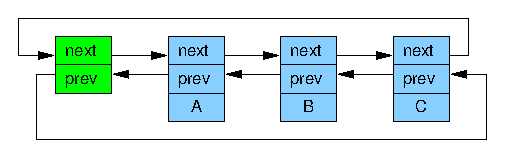
\includegraphics{defer/Linux_list}}
\caption{Linux Circular Linked List (\tco{list})}
\label{fig:defer:Linux Circular Linked List (list)}
\end{figure}

\begin{figure}
\centering
\resizebox{3in}{!}{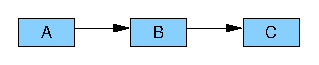
\includegraphics{defer/Linux_list_abbr}}
\caption{Linux Linked List Abbreviated}
\label{fig:defer:Linux Linked List Abbreviated}
\end{figure}

Although \co{rcu_assign_pointer()} and
\co{rcu_dereference()} can in theory be used to construct any
conceivable RCU-protected data structure, in practice it is often better
to use higher-level constructs.
Therefore, the \co{rcu_assign_pointer()} and
\co{rcu_dereference()}
primitives have been embedded in special RCU variants of Linux's
list-manipulation API\@.
Linux has four variants of doubly linked list, the circular
\co{struct list_head} and the linear
\co{struct hlist_head}/\co{struct hlist_node},
\co{struct hlist_nulls_head}/\co{struct hlist_nulls_node}, and
\co{struct hlist_bl_head}/\co{struct hlist_bl_node}
pairs.
The former is laid out as shown in
\cref{fig:defer:Linux Circular Linked List (list)},
where the green (leftmost) boxes represent the list header and the blue
(rightmost three) boxes represent the elements in the list.
This notation is cumbersome, and will therefore be abbreviated as shown in
\cref{fig:defer:Linux Linked List Abbreviated},
which shows only the non-header (blue) elements.

\begin{figure}
\centering
\resizebox{3in}{!}{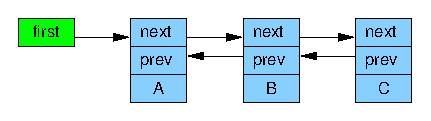
\includegraphics{defer/Linux_hlist}}
\caption{Linux Linear Linked List (\tco{hlist})}
\label{fig:defer:Linux Linear Linked List (hlist)}
\end{figure}

Linux's \co{hlist}\footnote{
	The ``h'' stands for hashtable, in which it reduces memory
	use by half compared to Linux's double-pointer circular
	linked list.}
is a linear list, which means that
it needs only one pointer for the header rather than the two
required for the circular list, as shown in
\cref{fig:defer:Linux Linear Linked List (hlist)}.
Thus, use of \co{hlist} can halve the memory consumption for the hash-bucket
arrays of large hash tables.
As before, this notation is cumbersome, so \co{hlist} structures will
be abbreviated in the same way \co{list_head}-style lists are, as shown in
\cref{fig:defer:Linux Linked List Abbreviated}.

A variant of Linux's \co{hlist}, named \co{hlist_nulls}, provides multiple
distinct \co{NULL} pointers, but otherwise uses the same layout as shown in
\cref{fig:defer:Linux Linear Linked List (hlist)}.
In this variant, a \co{->next} pointer having a zero low-order bit is
considered to be a pointer.
However, if the low-order bit is set to one, the upper bits identify
the type of \co{NULL} pointer.
This type of list is used to allow lockless readers to detect when a
node has been moved from one list to another.
For example, each bucket of a hash table might use its index to mark
its \co{NULL} pointer.
Should a reader encounter a \co{NULL} pointer not matching the index of
the bucket it started from, that reader knows that an element it was
traversing was moved to some other bucket during the traversal, taking
that reader with it.
The reader can use the \apik{is_a_nulls()} function (which returns \co{true}
if passed an \co{hlist_nulls} \co{NULL} pointer) to determine when
it reaches the end of a list, and the \apik{get_nulls_value()} function
(which returns its argument's \co{NULL}-pointer identifier) to fetch
the type of \co{NULL} pointer.
When \co{get_nulls_value()} returns an unexpected value, the reader
can take corrective action, for example, restarting its traversal from
the beginning.

\QuickQuiz{
	But what if an \co{hlist_nulls} reader gets moved to some other
	bucket and then back again?
}\QuickQuizAnswer{
	One way to handle this is to always move nodes to the beginning
	of the destination bucket, ensuring that when the reader reaches
	the end of the list having a matching \co{NULL} pointer, it will
	have searched the entire list.

	Of course, if there are too many move operations in a hash table
	with many elements per bucket, the reader might never reach the
	end of a list.
	One way of avoiding this in the common case is to keep hash
	tables well-tuned, thus with short lists.
	One way of detecting the problem and handling it is for the
	reader to terminate the search after traversing some large
	number of nodes, acquire the update-side lock, and redo the
	search, but this might introduce deadlocks.
	Another way of avoiding the problem entirely is for readers to
	search within RCU read-side critical sections, and to wait for
	an RCU grace period between successive updates.
	An intermediate position might wait for an RCU grace period
	every $N$ updates, for some suitable value of $N$.
}\QuickQuizEnd

More information on \co{hlist_nulls} is available in the Linux-kernel
source tree, with helpful example code provided in the
\path{rculist_nulls.rst} file (\path{rculist_nulls.txt} in older kernels).

Another variant of Linux's \co{hlist} incorporates bit-locking,
and is named \co{hlist_bl}.
This variant uses the same layout as shown in
\cref{fig:defer:Linux Linear Linked List (hlist)},
but reserves the low-order bit of the head pointer (``first'' in the
figure) to lock the list.
This approach also reduces memory usage, as it allows what would otherwise
be a separate spinlock to be stored with the pointer itself.

\begin{sidewaystable*}[htbp]
\rowcolors{1}{}{lightgray}
\renewcommand*{\arraystretch}{1.3}
\centering
\caption{RCU-Protected List APIs}
\label{tab:defer:RCU-Protected List APIs}
\footnotesize
\newlength{\cwa}\newlength{\cwb}\newlength{\cwc}\newlength{\cwd}
\IfNimbusAvail{
  \renewcommand{\ttdefault}{NimbusMonoN}
  \setlength{\cwa}{1.9in}\setlength{\cwb}{2.1in}
  \setlength{\cwc}{1.8in}\setlength{\cwd}{1.6in}
}{
  \setlength{\cwa}{1.95in}\setlength{\cwb}{2.15in}
  \setlength{\cwc}{1.9in}\setlength{\cwd}{1.7in}
}
\ebresizewidthsw{
\begin{tabular}{>{\raggedright\arraybackslash}p{\cwa}
    >{\raggedright\arraybackslash}p{\cwb}
    >{\raggedright\arraybackslash}p{\cwc}
    >{\raggedright\arraybackslash}p{\cwd}}
\toprule
\pmb{\tco{list}}: Circular doubly linked list &
    \pmb{\tco{hlist}}: Linear doubly linked list &
	\pmb{\tco{hlist_nulls}}: Linear doubly linked list with marked
	NULL pointer, with up to 31~bits of marking &
	    \pmb{\tco{hlist_bl}}: Linear doubly linked list with bit locking \\
\midrule
\multicolumn{4}{l}{{\bf Structures}} \\
\tco{struct list_head} &
    \tco{struct}{\tt ~}\tco{hlist_head} ~~~~~~~~~~~~~~
    \tco{struct}{\tt ~}\tco{hlist_node} &
	\tco{struct}{\tt ~}\tco{hlist_nulls_head}
	\tco{struct}{\tt ~}\tco{hlist_nulls_node} &
	    \tco{struct}{\tt ~}\tco{hlist_bl_head}
	    \tco{struct}{\tt ~}\tco{hlist_bl_node} \\
\multicolumn{4}{l}{{\bf Initialization}} \\
\tco{INIT_LIST_HEAD_RCU()} &
    &
	&
	    \\
\multicolumn{4}{l}{{\bf Full traversal}} \\
\tco{list_for_each_entry_rcu()}
\tco{list_for_each_entry_lockless()}
\tco{list_for_each_entry_srcu()} &
    \tco{hlist_for_each_entry_rcu()}
    \tco{hlist_for_each_entry_rcu_bh()}
    \tco{hlist_for_each_entry_rcu_notrace()}
    \tco{hlist_for_each_entry_srcu()} &
	\tco{hlist_nulls_for_each_entry_rcu()}
	\tco{hlist_nulls_for_each_entry_safe()} &
	    \tco{hlist_bl_for_each_entry_rcu()} \\
\multicolumn{4}{l}{{\bf Resume traversal}} \\
\tco{list_for_each_entry_continue_rcu()}
\tco{list_for_each_entry_from_rcu()} &
    \tco{hlist_for_each_entry_continue_rcu()}
    \tco{hlist_for_each_entry_continue_rcu_bh()}
    \tco{hlist_for_each_entry_from_rcu()} &
	&
	    \\
\multicolumn{4}{l}{{\bf Stepwise traversal}} \\
\tco{list_entry_rcu()}
\tco{list_entry_lockless()}
\tco{list_first_or_null_rcu()}
\tco{list_next_rcu()}
\tco{list_next_or_null_rcu()}
\tco{list_tail_rcu()} &
    \multicolumn{1}{p{1.2in}}{\tco{hlist_first_rcu()}
			      \tco{hlist_next_rcu()}
			      \tco{hlist_pprev_rcu()}} &
	\tco{hlist_nulls_first_rcu()}
	\tco{hlist_nulls_next_rcu()} &
	    \tco{hlist_bl_first_rcu()} \\
\multicolumn{4}{l}{{\bf Add}} \\
\multicolumn{1}{p{1.2in}}{\tco{list_add_rcu()}
			  \tco{list_add_tail_rcu()}} &
    \tco{hlist_add_before_rcu()}
    \tco{hlist_add_behind_rcu()}
    \tco{hlist_add_head_rcu()}
    \tco{hlist_add_tail_rcu()} &
	\tco{hlist_nulls_add_head_rcu()}
	\tco{hlist_nulls_add_tail_rcu()}
	\tco{hlist_nulls_add_fake()} &
	    \tco{hlist_bl_add_head_rcu()}
	    \tco{hlist_bl_set_first_rcu()} \\
\multicolumn{4}{l}{{\bf Delete}} \\
\tco{list_del_rcu()} &
    \multicolumn{1}{p{1.2in}}{\tco{hlist_del_rcu()}
			      \tco{hlist_del_init_rcu()}} &
	\tco{hlist_nulls_del_rcu()}
	\tco{hlist_nulls_del_init_rcu()} &
	    \tco{hlist_bl_del_rcu()} \\
\multicolumn{4}{l}{{\bf Replace}} \\
\tco{list_replace_rcu()} &
    \tco{hlist_replace_rcu()} &
	&
	    \\
\multicolumn{4}{l}{{\bf Splice}} \\
\tco{list_splice_init_rcu()}
\tco{list_splice_tail_init_rcu()} &
    \tco{hlists_swap_heads_rcu()} &
	&
	    \\
\bottomrule
\end{tabular}
}
\end{sidewaystable*}

The API members for these linked-list variants are summarized in
\cref{tab:defer:RCU-Protected List APIs}.
More information is available in the \path{Documentation/RCU}
directory of the Linux-kernel source tree and at
Linux Weekly News~\cite{PaulEMcKenney2024RCUAPI}.

However, the remainder of this section expands on the use of
\apik{list_replace_rcu()}, given that this API member gave RCU its name.
This API member is used to carry out more complex updates in which an
element in the middle of the list having multiple fields is atomically
updated, so that a given reader sees either the old set of values or
the new set of values, but not a mixture of the two sets.
For example, each node of a linked list might have integer fields
\co{->a}, \co{->b}, and~\co{->c}, and it might be necessary to update
a given node's fields from 5, 6, and~7 to 5, 2, and~3, respectively.

The code implementing this atomic update is straightforward:

\begin{fcvlabel}[ln:defer:Canonical RCU Replacement Example (2nd)]
\begin{VerbatimN}[samepage=true,commandchars=\\\[\],firstnumber=15]
q = kmalloc(sizeof(*p), GFP_KERNEL);	\lnlbl[kmalloc]
*q = *p;				\lnlbl[copy]
q->b = 2;				\lnlbl[update1]
q->c = 3;				\lnlbl[update2]
list_replace_rcu(&p->list, &q->list);	\lnlbl[replace]
synchronize_rcu();			\lnlbl[sync_rcu]
kfree(p);				\lnlbl[kfree]
\end{VerbatimN}
\end{fcvlabel}

\begin{figure}
\centering
\IfEbookSize{
\resizebox{2in}{!}{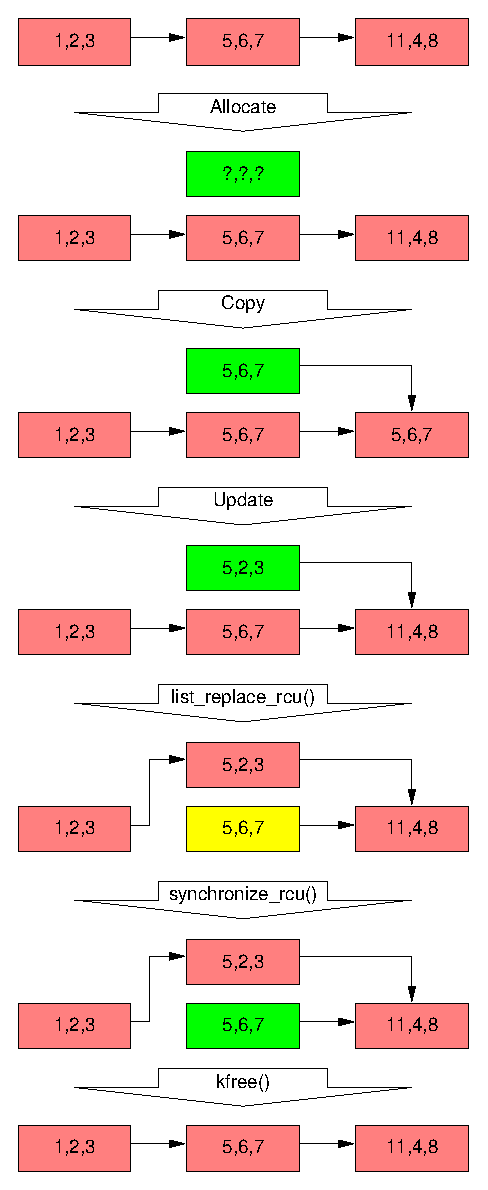
\includegraphics{defer/RCUReplacement}}
}{
\resizebox{2.7in}{!}{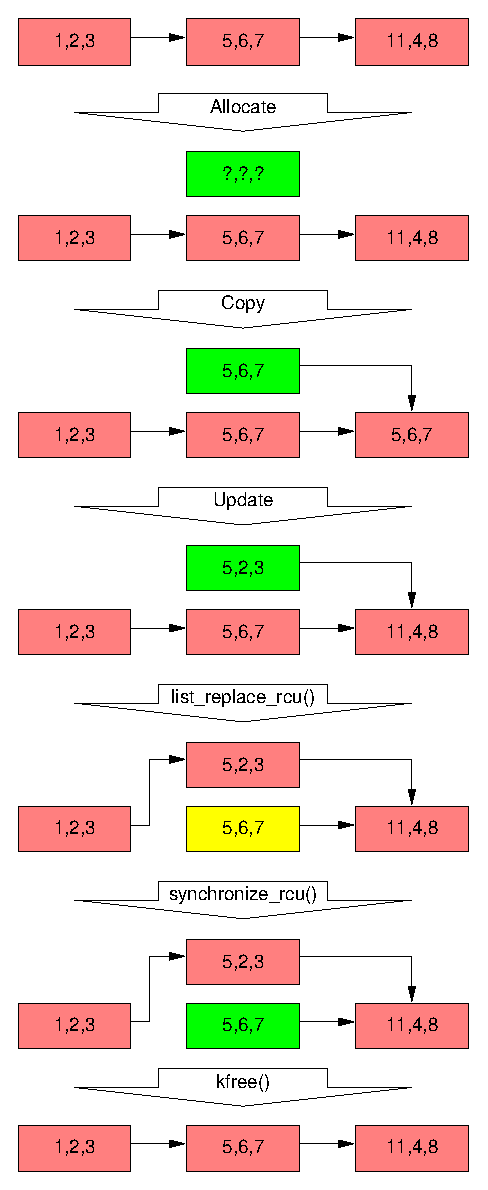
\includegraphics{defer/RCUReplacement}}
}
\caption{RCU Replacement in Linked List}
\label{fig:defer:RCU Replacement in Linked List}
\end{figure}

The following discussion walks through this code, using
\cref{fig:defer:RCU Replacement in Linked List} to illustrate
the state changes.
The triples in each element represent the values of fields \co{->a},
\co{->b}, and~\co{->c}, respectively.
The red-shaded elements might be referenced by readers,
and because readers do not synchronize directly with updaters,
readers might run concurrently with this entire replacement process.
Please note that backwards pointers and the link from the tail to the
head are omitted for clarity.

The initial state of the list, including the pointer \co{p},
is the same as for the deletion example, as shown on the
first row of the figure.

The following text describes how to replace the \co{5,6,7} element
with \co{5,2,3} in such a way that any given reader sees one of these
two values.

\begin{fcvref}[ln:defer:Canonical RCU Replacement Example (2nd)]
\Clnref{kmalloc} allocates a replacement element,
resulting in the state as shown in the second row of
\cref{fig:defer:RCU Replacement in Linked List}.
At this point, no reader can hold a reference to the newly allocated
element (as indicated by its green shading), and it is uninitialized
(as indicated by the question marks).

\Clnref{copy} copies the old element to the new one, resulting in the
state as shown in the third row of
\cref{fig:defer:RCU Replacement in Linked List}.
The newly allocated element still cannot be referenced by readers, but
it is now initialized.

\Clnref{update1} updates \co{q->b} to the value ``2'', and
\clnref{update2} updates \co{q->c} to the value ``3'',
as shown on the fourth row of
\cref{fig:defer:RCU Replacement in Linked List}.
Note that the newly allocated structure is still inaccessible to readers.

Now, \clnref{replace} does the replacement, so that the new element is
finally visible to readers, and hence is shaded red, as shown on
the fifth row of
\cref{fig:defer:RCU Replacement in Linked List}.
At this point, as shown below, we have two versions of the list.
Pre-existing readers might see the \co{5,6,7} element (which is
therefore now shaded yellow), but
new readers will instead see the \co{5,2,3} element.
But any given reader is guaranteed to see one set of values or the
other, not a mixture of the two.

After the \co{synchronize_rcu()} on \clnref{sync_rcu} returns,
a grace period will have elapsed, and so all reads that started before the
\apik{list_replace_rcu()} will have completed.
In particular, any readers that might have been holding references
to the \co{5,6,7} element are guaranteed to have exited
their RCU read-side critical sections, and are thus prohibited from
continuing to hold a reference.
Therefore, there can no longer be any readers holding references
to the old element, as indicated by its green shading in the sixth row of
\cref{fig:defer:RCU Replacement in Linked List}.
As far as the readers are concerned, we are back to having a single version
of the list, but with the new element in place of the old.

After the \apik{kfree()} on \clnref{kfree} completes, the list will
appear as shown on the final row of
\cref{fig:defer:RCU Replacement in Linked List}.
\end{fcvref}

Despite the fact that RCU was named after the replacement case,
the vast majority of RCU usage within the Linux kernel relies on
the simple independent insertion and deletion, as was shown in
\cref{fig:defer:Multiple RCU Data-Structure Versions} in
\cref{sec:defer:Maintain Multiple Versions of Recently Updated Objects}.

\QuickQuiz{
	Why doesn't
	\cref{tab:defer:RCU-Protected List APIs}
	include additional list-initialization APIs such as
	\co{INIT_HLIST_HEAD()}?
}\QuickQuizAnswer{
	Because this and similar APIs are not specific to RCU, but
	are also (and sometimes mainly) used for similar lists
	that are protected by other synchronization mechanisms.
}\QuickQuizEnd

The next section looks at APIs that assist developers in debugging
their code that makes use of RCU\@.

\subsubsection{RCU Has Diagnostic APIs}
\label{sec:defer:RCU Has Diagnostic APIs}

\begin{table}
\renewcommand*{\arraystretch}{1.15}
\footnotesize
\centering
\begin{tabular}{ll}
\toprule
Category &
	Primitives \\
\midrule
Mark RCU pointer &
	\tco{__rcu} \\
\midrule
Debug-object support &
	\tco{init_rcu_head()} \\
&	\tco{destroy_rcu_head()} \\
&	\tco{init_rcu_head_on_stack()} \\
&	\tco{destroy_rcu_head_on_stack()} \\
\midrule
Stall-warning control &
	\tco{rcu_cpu_stall_reset()} \\
\midrule
Callback checking &
	\tco{rcu_head_init()} \\
&	\tco{rcu_head_after_call_rcu()} \\
\midrule
lockdep support &
	\tco{rcu_read_lock_held()} \\
&	\tco{rcu_read_lock_bh_held()} \\
&	\tco{rcu_read_lock_sched_held()} \\
&	\tco{srcu_read_lock_held()} \\
&	\tco{rcu_is_watching()} \\
&	\tco{RCU_LOCKDEP_WARN()} \\
&	\tco{rcu_sleep_check()} \\
\bottomrule
\end{tabular}
\caption{RCU Diagnostic APIs}
\label{tab:defer:RCU Diagnostic APIs}
\end{table}

\Cref{tab:defer:RCU Diagnostic APIs}
shows RCU's diagnostic APIs.

The \co{__rcu} tag marks an RCU-protected pointer, for example,
\qtco{struct foo __rcu *p;}.
Pointers that might be passed to \co{rcu_dereference()} can be marked,
but pointers holding values returned from \co{rcu_dereference()}
should not be.
Providing these markings on variables, structure fields, function
parameters, and return values allows the Linux kernel's \co{sparse}
tool to detect situations where RCU-protected pointers are
incorrectly accessed using plain C-language loads and stores.

Debug-object support is automatic for any \apik{rcu_head} structures
that are part of a structure obtained from the Linux kernel's
memory allocators, but those building their own special-purpose
memory allocators can use \apik{init_rcu_head()} and \apik{destroy_rcu_head()}
at allocation and free time, respectively.
Those using \co{rcu_head} structures allocated on the function-call
stack (it happens!\@) may use \apik{init_rcu_head_on_stack()}
before first use and \apik{destroy_rcu_head_on_stack()} after last use,
but before returning from the function.
Debug-object support allows detection of bugs involving passing the
same \co{rcu_head} structure to \co{call_rcu()} and friends in
quick succession, which is the \co{call_rcu()} counterpart to the
infamous double-free class of memory-allocation bugs.

Stall-warning control is provided by \apik{rcu_cpu_stall_reset()}, which
allows the caller to suppress RCU CPU stall warnings for the remainder
of the current grace period.
RCU CPU stall warnings help pinpoint situations where an RCU read-side
critical section runs for an excessive length of time, and it is useful
for things like kernel debuggers to be able to suppress them, for example,
when encountering a breakpoint.

Callback checking is provided by \apik{rcu_head_init()} and
\apik{rcu_head_after_call_rcu()}.
The former is invoked on an \co{rcu_head} structure before it is passed
to \co{call_rcu()}, and then \co{rcu_head_after_call_rcu()} will
check to see if the callback has been invoked with the specified
function.

Support for lockdep~\cite{JonathanCorbet2006lockdep} includes
\apik{rcu_read_lock_held()},
\apik{rcu_read_lock_bh_held()},
\apik{rcu_read_lock_sched_held()}, and
\apik{srcu_read_lock_held()},
each of which returns \co{true} if invoked within the corresponding
type of RCU read-side critical section.

\QuickQuiz{
	Why isn't there a \co{rcu_read_lock_tasks_held()} for Tasks RCU?
}\QuickQuizAnswer{
	Because Tasks RCU does not have read-side markers.
	Instead, Tasks RCU read-side critical sections are
	bounded by voluntary context switches.
}\QuickQuizEnd

Because \co{rcu_read_lock()} cannot be used from the idle loop,
and because energy-efficiency concerns have caused the idle loop
to become quite ornate, \apik{rcu_is_watching()} returns \co{true} if
invoked in a context where use of \co{rcu_read_lock()} is legal.
Note again that \co{srcu_read_lock()} may be used from idle and
even offline CPUs, which means that \co{rcu_is_watching()} does not
apply to SRCU\@.

\apik{RCU_LOCKDEP_WARN()} emits a warning if lockdep is enabled and if
its argument evaluates to \co{true}.
For example, \co{RCU_LOCKDEP_WARN(!rcu_read_lock_held())} would emit a
warning if invoked outside of an RCU read-side critical section.

\apik{RCU_NONIDLE()} may be used to force RCU to watch when executing
the statement that is passed in as the sole argument.
For example, \co{RCU_NONIDLE(WARN_ON(!rcu_is_watching()))}
would never emit a warning.
However, changes in the 2020--2021 timeframe extend RCU's reach deeper
into the idle loop, which should greatly reduce or even eliminate the
need for \co{RCU_NONIDLE()}.

Finally,  \apik{rcu_sleep_check()} emits a warning if invoked within
an RCU, RCU-bh, or RCU-sched read-side critical section.

\subsubsection{Where Can RCU's APIs Be Used?}
\label{sec:defer:Where Can RCU's APIs Be Used?}

\begin{figure}
\centering
\resizebox{3in}{!}{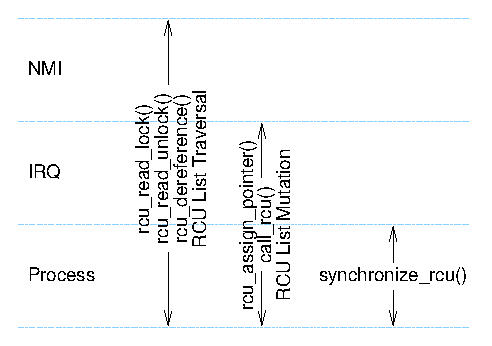
\includegraphics{defer/RCUenvAPI}}
\caption{RCU API Usage Constraints}
\label{fig:defer:RCU API Usage Constraints}
\end{figure}

\Cref{fig:defer:RCU API Usage Constraints}
shows which APIs may be used in which in-kernel environments.
The RCU read-side primitives may be used in any environment, including NMI,
the RCU mutation and asynchronous grace-period primitives may be used in any
environment other than NMI, and, finally, the RCU synchronous grace-period
primitives may be used only in process context.
The RCU list-traversal primitives include \apik{list_for_each_entry_rcu()},
\apik{hlist_for_each_entry_rcu()}, etc.
Similarly, the RCU list-mutation primitives include
\apik{list_add_rcu()}, \apik{hlist_del_rcu()}, etc.

Note that as a general rule, primitives from other families of RCU
may be substituted, although \co{srcu_read_lock_nmisafe()} but not
\co{srcu_read_lock()} may be used in NMI context.

\subsubsection{RCU in Userspace Applications?}
\label{sec:defer:RCU in Userspace Applications?}

The userspace RCU library uses a C-language API similar to that of
the kernel's core RCU API~\cite{PaulMcKenney2013LWNURCUAPI},
with extensions for
hash tables~\cite{PaulMcKenney2013LWNURCUhashAPI},
queues and stacks~\cite{PaulMcKenney2013LWNURCUqueuestackAPI},
atomic operations~\cite{PaulMcKenney2013LWNURCUatomicop}, and
linked lists~\cite{PaulMcKenney2013LWNURCUlist}.

\begin{table*}
\rowcolors{1}{}{lightgray}
\renewcommand*{\arraystretch}{1.15}
\footnotesize
\centering\OneColumnHSpace{-.4in}
\ebresizewidth{
\begin{tabular}{ll}
\toprule
\multicolumn{1}{c}{Linux Kernel} &
	\multicolumn{1}{c}{C++26} \\
\midrule
\tco{guard(rcu)()} &
	\tco{std::scoped_lock l(std::rcu_default_domain())} \\
\tco{rcu_read_lock()} &
	\tco{std::rcu_default_domain().lock()} \\
\tco{rcu_read_unlock()} &
	\tco{std::rcu_default_domain().unlock()} \\
\tco{synchronize_rcu()} &
	\tco{std::rcu_synchronize()} \\
\tco{struct rcu_head} &
	\tco{std::rcu_obj_base<T>} \\
\tco{call_rcu()} &
	\tco{std::rcu_obj_base<T> .retire()} \\
\tco{kfree_rcu_mightsleep()} &
	\tco{std::rcu_retire()} \\
\tco{rcu_barrier()} &
	\tco{std::rcu_barrier()} \\
\bottomrule
\end{tabular}
}
\caption{RCU API Decoder Ring For Linux Kernel and C++26}
\label{tab:defer:RCU API Decoder Ring For Linux Kernel and C++26}
\end{table*}

Although the userspace RCU library has served well for many years as the
defacto definition of the C-language userspace RCU API, in 2023 the RCU
API was added to the C++26 draft
standard~\cite{PaulEMcKennney2023C++26RCU4,ThomasKoeppe2025N5032}.
The mapping from the Linux-kernel RCU API to that of
C++~\cite{PaulEMcKenney2023P0124R8-LKMM,PaulEMcKenney2026cppRCU}
is shown in
\cref{tab:defer:RCU API Decoder Ring For Linux Kernel and C++26}.
The many differences between C and C++ do complicate this mapping.

The \co{std::rcu_default_domain()} function returns a reference to
the only possible member of the \co{rcu_domain} class, which is provided
solely to permit RCU readers to be managed by the existing C++ scoped-locking
API members, in this case, \co{std::scoped_lock}.
A future version of the C++ standard might provide for multiple
\co{rcu_domain} objects, perhaps similar to Linux-kernel SRCU, but in
the meantime, there can only be one.
In cases where scoped RCU readers are not sufficient, the \co{rcu_domain}
object's \co{.lock()} and \co{.unlock()} member functions may be
invoked directly, providing the same capabilities (and risks) as do
\co{rcu_read_lock()} and \co{rcu_read_unlock()}.

Perhaps the Linux kernel's \co{synchronize_rcu()} should have instead been
named \co{rcu_synchronize()}, but the historical path from the pre-existing
\co{synchronize_irq()} to \co{synchronize_kernel()} to \co{synchronize_rcu()}
forced the Linux kernel's naming.

In the Linux kernel, you embed an \co{rcu_head} structure into your
RCU-protected structure in order to use \co{call_rcu()} and friends.
Given the C++ object orientation, you instead make your RCU-protected
class inherit from the \co{std::rcu_obj_base} class.
Instead of invoking a free function like \co{call_rcu()}, you use the
\co{rcu_obj_base} class's \co{.retire()} member function, which is the C++
counterpart to \co{call_rcu()} when a \emph{deleter} function is supplied
to \co{.retire()} and the C++ counterpart to \co{kfree_rcu()} otherwise.
C++ also supplies an \co{std::rcu_retire()} free function, which can be
passed objects which do not inherit from \co{std::rcu_obj_base}, just
as structures passed to the Linux kernel's \co{kfree_rcu_mightsleep()}
need not include an \co{rcu_head} structure.

However, the Linux kernel's \co{rcu_barrier()} function maps directly
to the C++ \co{std::rcu_barrier()} free function.

An additional complication stems from the C++ language's need to support
minimal unhosted and freestanding platforms.
Such platforms might not be able to create background threads, which
means that they must be permitted to drive RCU's grace-period state machine
forward from calls to \co{.retire()} and \co{rcu_retire()}.
This in turn means that these two functions must be permitted to
invoke RCU deleters (C++'s counterparts to the Linux kernel's RCU
callback function) from within a call to either \co{.retire()} or
\co{rcu_retire()}.
Therefore, in C++ (but not in the Linux kernel), fully portable C++ code
cannot hold a mutex across either \co{.retire()} or \co{rcu_retire()} if
that mutex is acquired by \emph{any} deleter that is passed to \emph{any}
invocation of \co{.retire()} or \co{rcu_retire()} \emph{anywhere} in
the application.

In short, although there are many similarities between Linux-kernel RCU
and C++ RCU, there are many important differences.
It will be interesting to see how both APIs evolve over time, and also
how RCU will be used in other languages, for example, Rust.

\subsubsection{So, What \emph{is} RCU Really?}
\label{sec:defer:So; What is RCU Really?}

Again, the core concept behind RCU is nothing more than updaters waiting
for all pre-existing readers to complete, but neither blocking nor
necessarily being blocked by new readers.

This core concept is augmented by different techniques for different
RCU use cases.
The most common use case adds APIs that support publication and
subscription for insertions and removals for deletions.
Additional use cases also build on top of RCU's core concept, including
the reader-writer-locking, reference-counting, existence-guarantee,
and others presented in
\cref{sec:defer:RCU Usage}.
Furthermore, I have no doubt that the Linux community will continue to
find interesting new uses for RCU, as they have over more than two
decades~\cite{PaulEMcKenney2008WhatIsRCUAPI,PaulEMcKenney2024RCUAPI}
and as they also do for any of a number of other synchronization primitives
throughout the kernel.

However, for many people, a complete view of RCU must include sample
RCU implementations.
\Cref{chp:app:``Toy'' RCU Implementations} therefore presents a series
of ``toy'' RCU implementations of increasing complexity and capability,
though others might prefer the classic
``User-Level Implementations of Read-Copy
Update''~\cite{MathieuDesnoyers2012URCU}.
For everyone else, the next section gives an overview of some RCU use cases.

% defer/rcuusage.tex
% mainfile: ../perfbook.tex
% SPDX-License-Identifier: CC-BY-SA-3.0

\subsection{RCU Usage}
\label{sec:defer:RCU Usage}
\OriginallyPublished{sec:defer:RCU Usage}{RCU Usage}{Linux Weekly News}{PaulEMcKenney2008WhatIsRCUUsage}

This section answers the question ``What is RCU?'' from the viewpoint
of the uses to which RCU can be put.
Because RCU is most frequently used to replace some existing mechanism,
we look at it primarily in terms of its relationship to such mechanisms,
as listed in \cref{tab:defer:RCU Usage}
and as displayed in \cref{fig:defer:Relationships Between RCU Use Cases}.
Following the sections listed in this table,
\cref{sec:defer:RCU Usage Summary} provides a summary,
which is expanded on in the following sections and
elsewhere~\cite{PaulEMcKenney2021RCUMysteriesFundamental,PaulEMcKenney2022RCUMysteriesUseCases}.

\begin{table}
\renewcommand*{\arraystretch}{1.2}
\centering
\small
\begin{tabular}{ll}
\toprule
Mechanism RCU Replaces & Page \\
\midrule
RCU for pre-BSD routing &
	\pageref{sec:defer:RCU for Pre-BSD Routing} \\
Wait for pre-existing things to finish &
	\pageref{sec:defer:Wait for Pre-Existing Things to Finish} \\
Phased state change &
	\pageref{sec:defer:Phased State Change} \\
Add-only list (publish/subscribe) &
	\pageref{sec:defer:Add-Only List} \\
Type-safe memory &
	\pageref{sec:defer:Type-Safe Memory} \\
Existence Guarantee &
	\pageref{sec:defer:Existence Guarantee} \\
Light-weight garbage collector &
	\pageref{sec:defer:Light-Weight Garbage Collector} \\
Delete-only list &
	\pageref{sec:defer:Delete-Only List} \\
Quasi reader-writer lock &
	\pageref{sec:defer:Quasi Reader-Writer Lock} \\
Quasi reference count &
	\pageref{sec:defer:Quasi Reference Count} \\
Quasi multi-version concurrency control (MVCC) &
	\pageref{sec:defer:Quasi Multi-Version Concurrency Control} \\
\bottomrule
\end{tabular}
\caption{RCU Usage}
\label{tab:defer:RCU Usage}
\end{table}

\subsubsection{RCU for Pre-BSD Routing}
\label{sec:defer:RCU for Pre-BSD Routing}

In contrast to the later sections, this section focuses on a very
specific use case for the purpose of comparison with other mechanisms.

\Cref{lst:defer:RCU Pre-BSD Routing Table Lookup,%
lst:defer:RCU Pre-BSD Routing Table Add/Delete}
show code for an RCU-protected Pre-BSD routing table
(\path{route_rcu.c}).
The former shows data structures and \co{route_lookup()},
and the latter shows \co{route_add()} and \co{route_del()}.

\begin{listing}
\input{CodeSamples/defer/route_rcu@lookup.fcv}
\caption{RCU Pre-BSD Routing Table Lookup}
\label{lst:defer:RCU Pre-BSD Routing Table Lookup}
\end{listing}

\begin{listing}
\input{CodeSamples/defer/route_rcu@add_del.fcv}
\caption{RCU Pre-BSD Routing Table Add/Delete}
\label{lst:defer:RCU Pre-BSD Routing Table Add/Delete}
\end{listing}

\begin{fcvref}[ln:defer:route_rcu:lookup]
In \cref{lst:defer:RCU Pre-BSD Routing Table Lookup},
\clnref{rh} adds the \co{->rh} field used by RCU reclamation,
\clnref{re_freed} adds the \co{->re_freed} use-after-free-check field,
\clnref{lock,unlock1,unlock2}
add RCU read-side protection,
and \clnref{chk_freed,abort} add the use-after-free check.
\end{fcvref}
\begin{fcvref}[ln:defer:route_rcu:add_del]
In \cref{lst:defer:RCU Pre-BSD Routing Table Add/Delete},
\clnref{add:lock,add:unlock,del:lock,%
del:unlock1,del:unlock2} add update-side locking,
\clnref{add:add_rcu,del:del_rcu} add RCU update-side protection,
\clnref{del:call_rcu} causes \co{route_cb()} to be invoked after
a grace period elapses,
and \clnrefrange{cb:b}{cb:e} define \co{route_cb()}.
This is minimal added code for a working concurrent implementation.
\end{fcvref}

\begin{figure}
\centering
\resizebox{2.5in}{!}{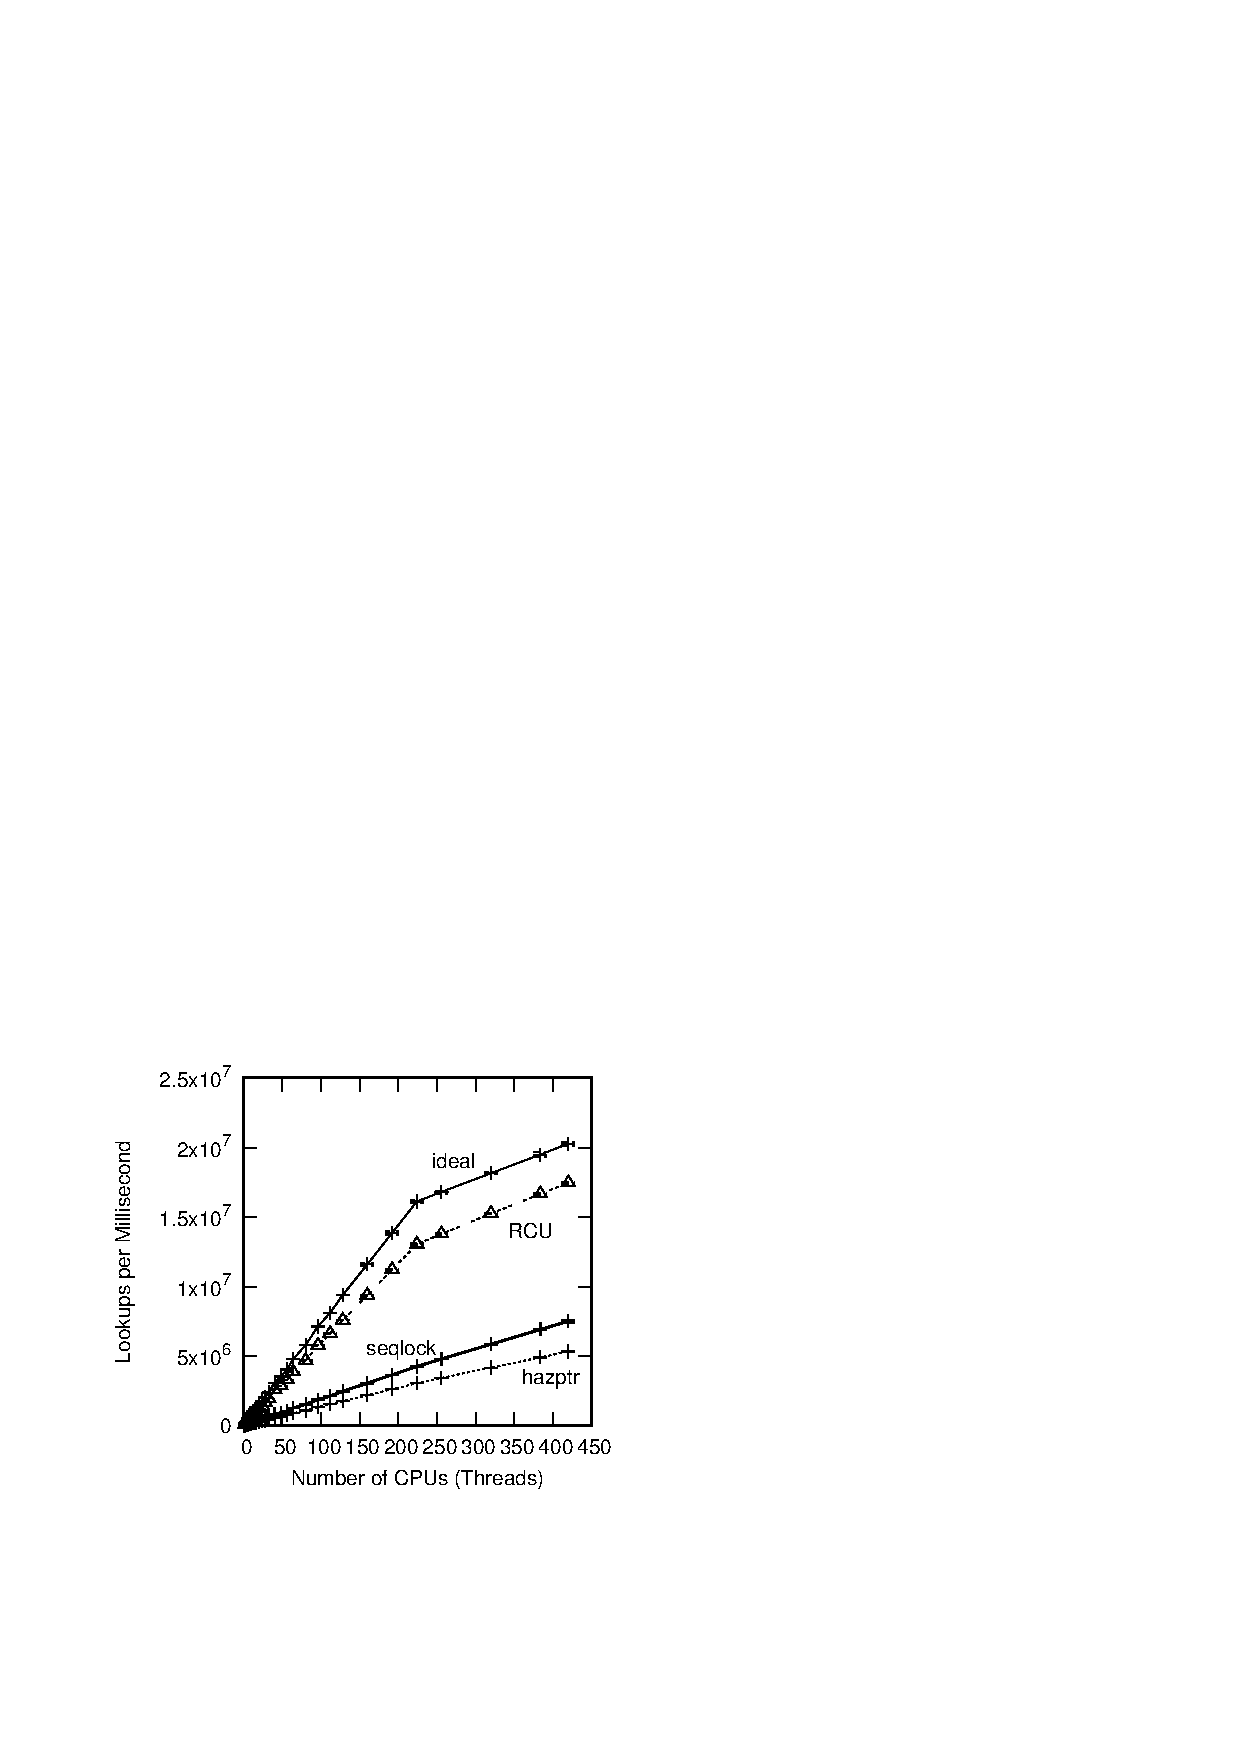
\includegraphics{CodeSamples/defer/data/hps.2019.12.17a/perf-rcu}}
\caption{Pre-BSD Routing Table Protected by RCU}
\label{fig:defer:Pre-BSD Routing Table Protected by RCU}
\end{figure}

\Cref{fig:defer:Pre-BSD Routing Table Protected by RCU}
shows the performance on the read-only workload.
RCU scales quite well, and offers nearly ideal performance.
However, this data was generated using the \co{RCU_SIGNAL}
flavor of userspace
RCU~\cite{MathieuDesnoyers2009URCU,PaulMcKenney2013LWNURCU},
for which \co{rcu_read_lock()} and \co{rcu_read_unlock()}
generate a small amount of code.
What happens for the \IXacr{qsbr} flavor of RCU, which generates no code at all
for \co{rcu_read_lock()} and \co{rcu_read_unlock()}?
(See \cref{sec:defer:Introduction to RCU},
and especially
\cref{fig:defer:QSBR: Waiting for Pre-Existing Readers},
for a discussion of RCU QSBR\@.)

The answer to this is shown in
\cref{fig:defer:Pre-BSD Routing Table Protected by RCU QSBR},
which shows that RCU QSBR's performance and scalability actually exceeds
that of the ideal synchronization-free workload.

\QuickQuizSeries{%
\QuickQuizB{
	Wait, what???
	How can RCU QSBR possibly be better than ideal?
	Just what rubbish definition of ideal would fail to be the best
	of all possible results???
}\QuickQuizAnswerB{
	This is an excellent question, and the answer is that modern
	CPUs and compilers are extremely complex.
	But before getting into that, it is well worth noting that
	RCU QSBR's performance advantage appears only in the
	one-hardware-thread-per-core regime.
	Once the system is fully loaded, RCU QSBR's performance drops
	back to ideal.

	The RCU variant of the \co{route_lookup()} search loop actually
	has one more x86 instruction than does the sequential version,
	namely the \co{lea} in the sequence
	\co{cmp}, \co{je}, \co{mov}, \co{cmp}, \co{lea}, and \co{jne}.
	This extra instruction is due to the \co{rcu_head} structure
	at the beginning of the RCU variant's \co{route_entry} structure,
	so that, unlike the sequential variant, the RCU variant's
	\co{->re_next.next} pointer has a non-zero offset.
	Back in the 1980s, this additional \co{lea} instruction might
	have reliably resulted in the RCU variant being slower, but we
	are now in the 21\textsuperscript{st} century, and the 1980s
	are long gone.

	But those of you who read
	\cref{sec:cpu:Pipelined CPUs}
	carefully already knew all of this!

	These counter-intuitive results of course mean that any
	performance result on modern microprocessors must be subject to
	some skepticism.
	In theory, it really does not make sense to obtain performance
	results that are better than ideal, but in practice, it really
	does happen on modern microprocessors.
	Such results can be thought of as similar to the celebrated
	super-linear speedups (see
	\cref{sec:SMPdesign:Beyond Partitioning}
	for one such example), that is, of interest but also of limited
	practical importance.
	Nevertheless, one of the strengths of RCU is that its read-side
	overhead is so low that tiny effects such as this one are visible
	in real performance measurements.

\begin{figure}
\centering
% Run with initial rcu_head structure in route_entry moved down.
\resizebox{2.5in}{!}{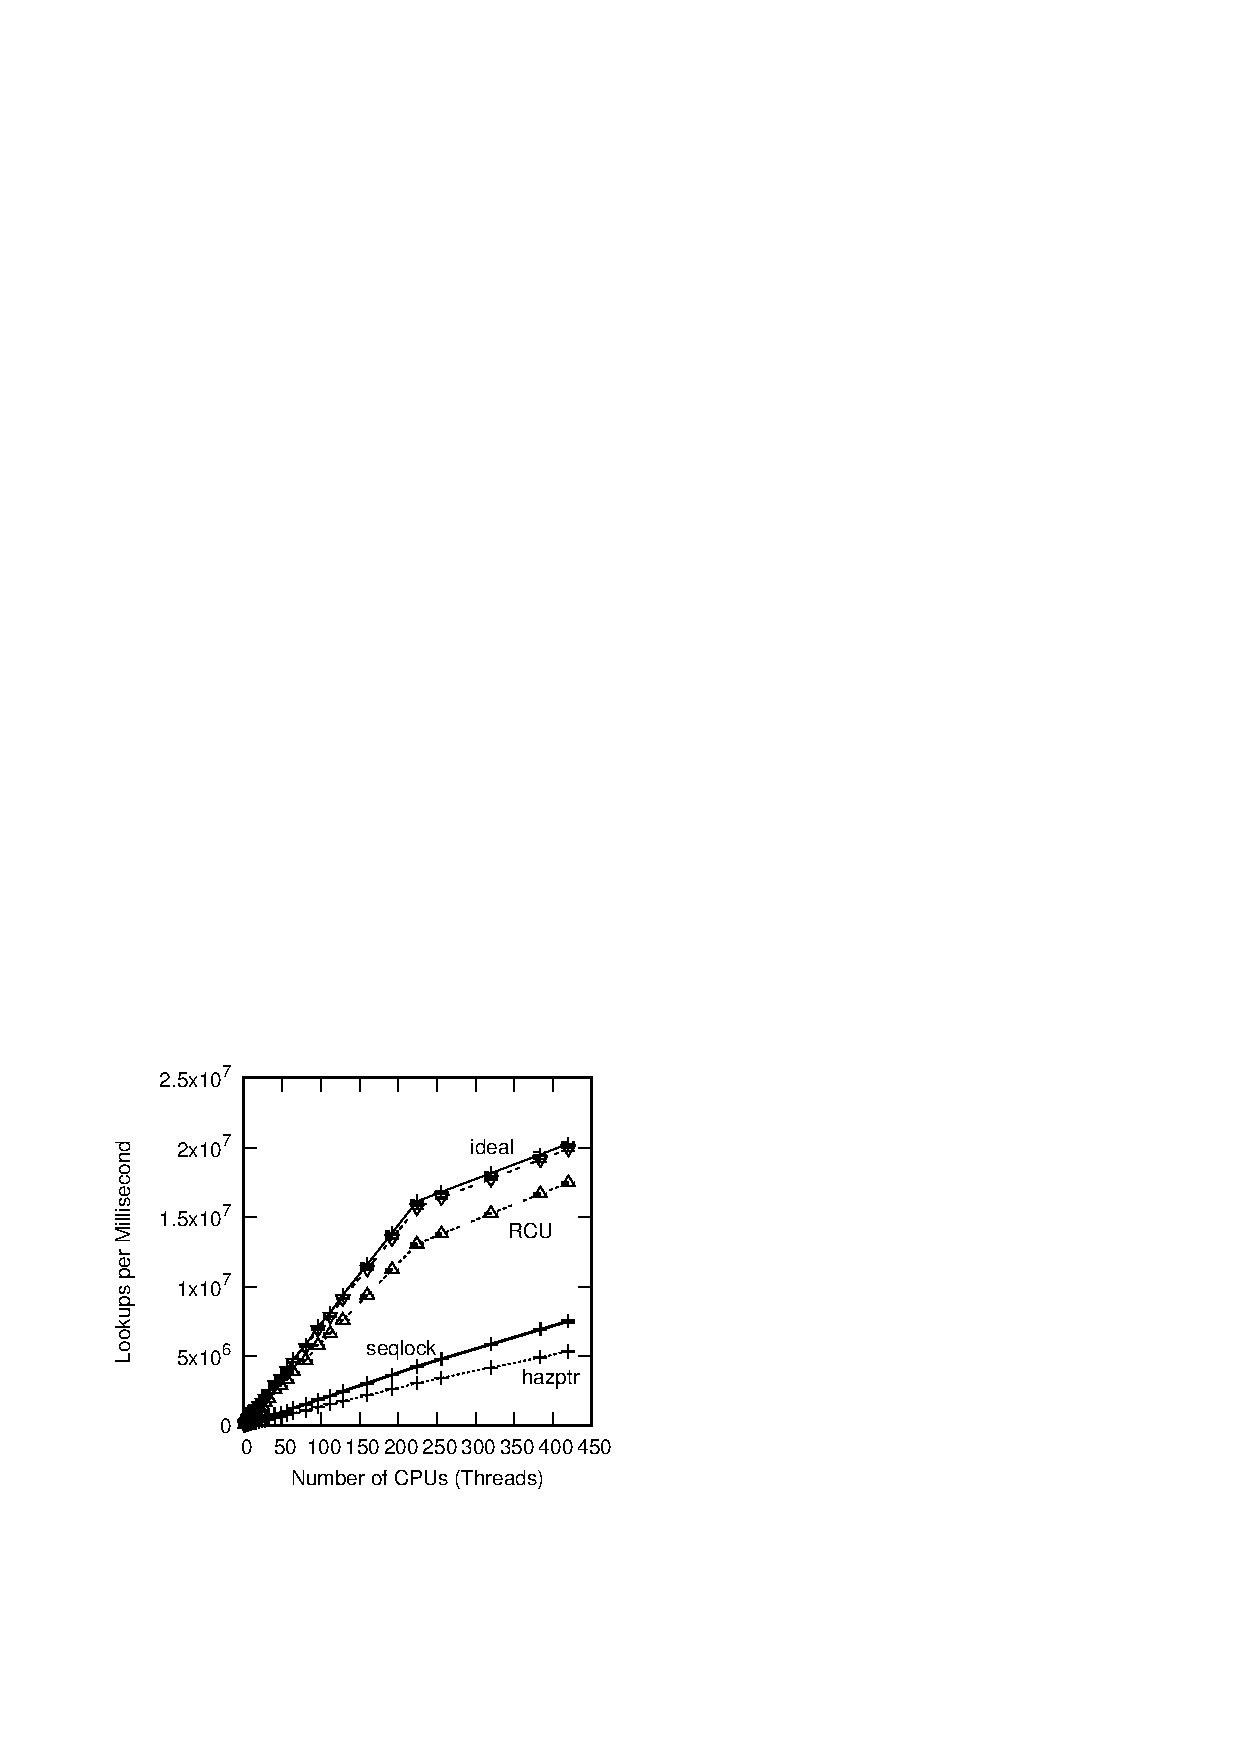
\includegraphics{CodeSamples/defer/data/hps.2019.12.17a/perf-rcu-qsbr}}
\caption{Pre-BSD Routing Table Protected by RCU QSBR With Non-Initial \tco{rcu_head}}
\label{fig:defer:Pre-BSD Routing Table Protected by RCU QSBR With Non-Initial rcu-head}
\end{figure}

	This raises the question as to what would happen if the
	\co{rcu_head} structure were to be moved so that RCU's
	\co{->re_next.next} pointer also had zero offset, just the
	same as the sequential variant.
	And the answer, as can be seen in
	\cref{fig:defer:Pre-BSD Routing Table Protected by RCU QSBR With Non-Initial rcu-head},
	is that this causes RCU QSBR's performance to decrease to where
	it is still very nearly ideal, but no longer super-ideal.
}\QuickQuizEndB
%
\QuickQuizE{
	Given RCU QSBR's read-side performance, why bother with any
	other flavor of userspace RCU?
}\QuickQuizAnswerE{
	Because RCU QSBR places constraints on the overall application
	that might not be tolerable,
	for example, requiring that each and every thread in the
	application regularly pass through a quiescent state.
	Among other things, this means that RCU QSBR is not helpful
	to library writers, who might be better served by other
	flavors of userspace RCU~\cite{PaulMcKenney2013LWNURCU}.
}\QuickQuizEndE
}

\begin{figure}
\centering
% Run with initial rcu_head structure at beginning of route_entry structure.
% This need to run twice is the reason for the oddball directory.
% @@@ Make this generate both files with a single run?
\resizebox{2.5in}{!}{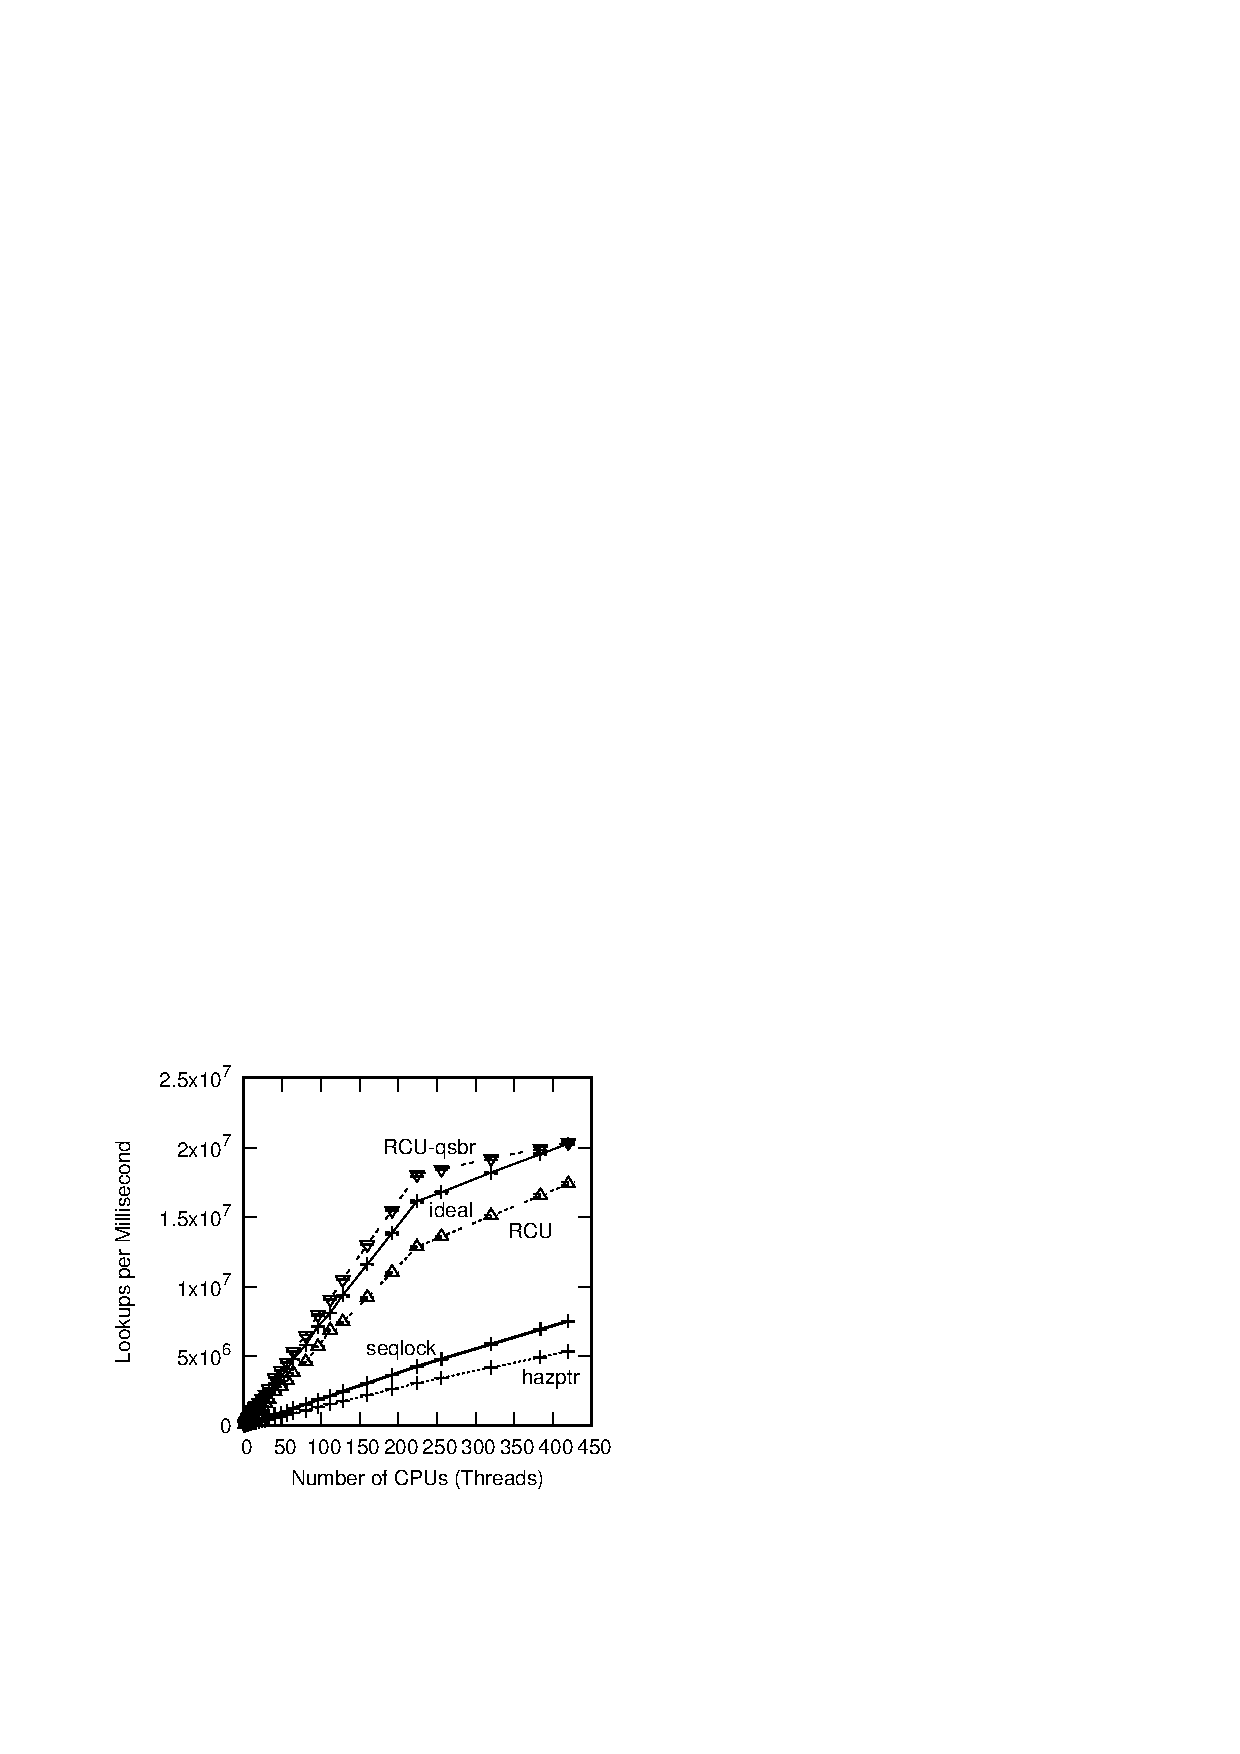
\includegraphics{CodeSamples/defer/data/hps.2019.12.02a/perf-rcu-qsbr}}
\caption{Pre-BSD Routing Table Protected by RCU QSBR}
\label{fig:defer:Pre-BSD Routing Table Protected by RCU QSBR}
\end{figure}

\begin{figure*}
\centering
\IfTwoColumn{
  \resizebox{5.5in}{!}{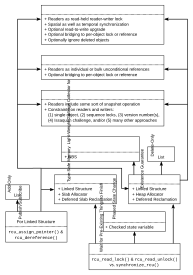
\includegraphics{defer/RCUusecases}}
}{
  \resizebox{.96\textwidth}{!}{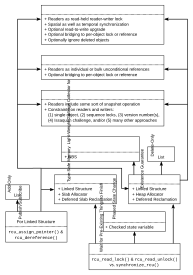
\includegraphics{defer/RCUusecases}}
  % eb builds require .96
}
\caption{Relationships Between RCU Use Cases}
\label{fig:defer:Relationships Between RCU Use Cases}
\end{figure*}

Although Pre-BSD routing is an excellent RCU use case, it is worthwhile
looking at the relationships between the wider spectrum of use cases
shown in
\cref{fig:defer:Relationships Between RCU Use Cases}.
This task is taken up by the following sections.

While reading these sections, please ask yourself which of these
use cases best describes Pre-BSD routing.

\subsubsection{Wait for Pre-Existing Things to Finish}
\label{sec:defer:Wait for Pre-Existing Things to Finish}

As noted in \cref{sec:defer:RCU Fundamentals}
an important component
of RCU is a way of waiting for RCU readers to finish.
One of
RCU's great strengths is that it allows you to wait for each of
thousands of different things to finish without having to explicitly
track each and every one of them, and without incurring
the performance degradation, scalability limitations, complex deadlock
scenarios, and memory-leak hazards that are inherent in schemes that
use explicit tracking.

In this section, we will show how \co{synchronize_sched()}'s
read-side counterparts (which include anything that disables preemption,
along with hardware operations and
primitives that disable interrupts) permit you to interact with
non-maskable interrupt
(NMI) handlers, which is quite difficult using locking.
This approach has been called ``Pure RCU''~\cite{PaulEdwardMcKenneyPhD},
and it is used in a few places in the Linux kernel.

The basic form of such ``Pure RCU'' designs is as follows:

\begin{enumerate}
\item	Make a change, for example, to the way that the OS reacts to an NMI\@.
\item	Wait for all pre-existing read-side critical sections to
	completely finish (for example, by invoking the
	\co{synchronize_sched()} primitive).\footnote{
		In Linux kernel v5.1 and later, \co{synchronize_sched()} has
		been subsumed into \co{synchronize_rcu()}.}
	The key observation here is that subsequent RCU read-side critical
	sections are guaranteed to see whatever change was made.
\item	Clean up, for example, return status indicating that the
	change was successfully made.
\end{enumerate}

The remainder of this section presents example code adapted from
the Linux kernel.
In this example, the \co{nmi_stop()} function in the now-defunct
oprofile facility uses \co{synchronize_sched()} to ensure that all
in-flight NMI notifications have completed before freeing the associated
resources.
A simplified version of this code is shown in
\cref{lst:defer:Using RCU to Wait for NMIs to Finish}.

\begin{listing}
\begin{fcvlabel}[ln:defer:Using RCU to Wait for NMIs to Finish]
\begin{VerbatimL}[commandchars=\\\@\$]
struct profile_buffer {				\lnlbl@struct:b$
	long size;
	atomic_t entry[0];
};						\lnlbl@struct:e$
static struct profile_buffer *buf = NULL;	\lnlbl@struct:buf$

void nmi_profile(unsigned long pcvalue)		\lnlbl@nmi_profile:b$
{
	struct profile_buffer *p = rcu_dereference(buf);\lnlbl@nmi_profile:rcu_deref$

	if (p == NULL)				\lnlbl@nmi_profile:if_NULL$
		return;				\lnlbl@nmi_profile:ret:a$
	if (pcvalue >= p->size)			\lnlbl@nmi_profile:if_oor$
		return;				\lnlbl@nmi_profile:ret:b$
	atomic_inc(&p->entry[pcvalue]);		\lnlbl@nmi_profile:inc$
}						\lnlbl@nmi_profile:e$

void nmi_stop(void)				\lnlbl@nmi_stop:b$
{
	struct profile_buffer *p = buf;		\lnlbl@nmi_stop:fetch$

	if (p == NULL)				\lnlbl@nmi_stop:if_NULL$
		return;				\lnlbl@nmi_stop:ret$
	rcu_assign_pointer(buf, NULL);		\lnlbl@nmi_stop:NULL$
	synchronize_sched();			\lnlbl@nmi_stop:sync_sched$
	kfree(p);				\lnlbl@nmi_stop:kfree$
}						\lnlbl@nmi_stop:e$
\end{VerbatimL}
\end{fcvlabel}
\caption{Using RCU to Wait for NMIs to Finish}
\label{lst:defer:Using RCU to Wait for NMIs to Finish}
\end{listing}

\begin{fcvref}[ln:defer:Using RCU to Wait for NMIs to Finish:struct]
\Clnrefrange{b}{e} define a \co{profile_buffer} structure, containing a
size and an indefinite array of entries.
\Clnref{buf} defines a pointer to a profile buffer, which is
presumably initialized elsewhere to point to a dynamically allocated
region of memory.
\end{fcvref}

\begin{fcvref}[ln:defer:Using RCU to Wait for NMIs to Finish:nmi_profile]
\Clnrefrange{b}{e} define the \co{nmi_profile()} function,
which is called from within an NMI handler.
As such, it cannot be preempted, nor can it be interrupted by a normal
interrupt handler, however, it is still subject to delays due to cache misses,
ECC errors, and cycle stealing by other hardware threads within the same
core.
\Clnref{rcu_deref} gets a local pointer to the profile buffer using the
\co{rcu_dereference()} primitive to ensure memory ordering on
DEC Alpha, and
\clnref{if_NULL,ret:a} exit from this function if there is no
profile buffer currently allocated, while \clnref{if_oor,ret:b}
exit from this function if the \co{pcvalue} argument
is out of range.
Otherwise, \clnref{inc} increments the profile-buffer entry indexed
by the \co{pcvalue} argument.
Note that storing the size with the buffer guarantees that the
range check matches the buffer, even if a large buffer is suddenly
replaced by a smaller one.
\end{fcvref}

\begin{fcvref}[ln:defer:Using RCU to Wait for NMIs to Finish:nmi_stop]
\Clnrefrange{b}{e} define the \co{nmi_stop()} function,
where the caller is responsible for mutual exclusion (for example,
holding the correct lock).
\Clnref{fetch} fetches a pointer to the profile buffer, and
\clnref{if_NULL,ret} exit the function if there is no buffer.
Otherwise, \clnref{NULL} \co{NULL}s out the profile-buffer pointer
(using the \co{rcu_assign_pointer()} primitive to maintain
memory ordering on weakly ordered machines),
and \clnref{sync_sched} waits for an RCU Sched grace period to elapse,
in particular, waiting for all non-preemptible regions of code,
including NMI handlers, to complete.
Once execution continues at \clnref{kfree}, we are guaranteed that
any instance of \co{nmi_profile()} that obtained a
pointer to the old buffer has returned.
It is therefore safe to free the buffer, in this case using the
\co{kfree()} primitive.
\end{fcvref}

\QuickQuiz{
	Suppose that the \co{nmi_profile()} function was preemptible.
	What would need to change to make this example work correctly?
}\QuickQuizAnswer{
	One approach would be to use
	\co{rcu_read_lock()} and \co{rcu_read_unlock()}
	in \co{nmi_profile()}, and to replace the
	\co{synchronize_sched()} with \co{synchronize_rcu()},
	perhaps as shown in
	\cref{lst:defer:Using RCU to Wait for Mythical Preemptible NMIs to Finish}.
%
\begin{listing}
\begin{VerbatimL}
struct profile_buffer {
	long size;
	atomic_t entry[0];
};
static struct profile_buffer *buf = NULL;

void nmi_profile(unsigned long pcvalue)
{
	struct profile_buffer *p;

	rcu_read_lock();
	p = rcu_dereference(buf);
	if (p == NULL) {
		rcu_read_unlock();
		return;
	}
	if (pcvalue >= p->size) {
		rcu_read_unlock();
		return;
	}
	atomic_inc(&p->entry[pcvalue]);
	rcu_read_unlock();
}

void nmi_stop(void)
{
	struct profile_buffer *p = buf;

	if (p == NULL)
		return;
	rcu_assign_pointer(buf, NULL);
	synchronize_rcu();
	kfree(p);
}
\end{VerbatimL}
\caption{Using RCU to Wait for Mythical Preemptible NMIs to Finish}
\label{lst:defer:Using RCU to Wait for Mythical Preemptible NMIs to Finish}
\end{listing}

	But why on earth would an NMI handler be preemptible???
}\QuickQuizEnd

In short, RCU makes it easy to dynamically switch among profile
buffers (you just \emph{try} doing this efficiently with atomic
operations, or at all with locking!).
This is a rare use of RCU in its pure form.
RCU is normally used at higher levels of abstraction, as
will be shown in the following sections.

\subsubsection{Phased State Change}
\label{sec:defer:Phased State Change}

\Cref{fig:defer:Phased State Change for Maintenance Operation}
shows a timeline for an example phased state change to efficiently
handle maintenance operations.
If there is no maintenance operation in progress, common-case operations
must proceed quickly, for example, without acquiring a reader-writer lock.
However, if there is a maintenance operation in progress, the common-case
operations must be undertaken carefully, taking into account added
complexities due to their running concurrently with that maintenance
operation.
This means that common-case operations will incur higher overhead during
maintenance operations, which is one reason that maintenance operations
are normally scheduled to take place during times of low load.

\begin{figure}
\centering
\resizebox{\twocolumnwidth}{!}{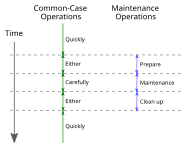
\includegraphics{defer/RCUphasedstatechange}}
\caption{Phased State Change for Maintenance Operation}
\label{fig:defer:Phased State Change for Maintenance Operation}
\end{figure}

In the figure, these apparently conflicting requirements are resolved by
having a prepare phase prior to the maintenance operation and a cleanup
phase after it, during which the common-case operations can proceed
either quickly or carefully.

\begin{listing}
\begin{fcvlabel}[ln:defer:Phased State Change for Maintenance Operations]
\begin{VerbatimL}[commandchars=\\\@\$]
bool be_careful;

void cco(void)
{
	rcu_read_lock();			\lnlbl@rrl$
	if (READ_ONCE(be_careful))		\lnlbl@if$
		cco_carefully();		\lnlbl@careful$
	else
		cco_quickly();			\lnlbl@quick$
	rcu_read_unlock();			\lnlbl@rul$
}

void maint(void)
{
	WRITE_ONCE(be_careful, true);		\lnlbl@tocareful$
	synchronize_rcu();			\lnlbl@sr1$
	do_maint();				\lnlbl@maint$
	synchronize_rcu();			\lnlbl@sr2$
	WRITE_ONCE(be_careful, false);		\lnlbl@toquick$
}
\end{VerbatimL}
\end{fcvlabel}
\caption{Phased State Change for Maintenance Operations}
\label{lst:defer:Phased State Change for Maintenance Operations}
\end{listing}

\begin{fcvref}[ln:defer:Phased State Change for Maintenance Operations]
Example pseudo-code for this phased state change is shown in
\cref{lst:defer:Phased State Change for Maintenance Operations}.
The common-case operations are carried out by \co{cco()} within an RCU
read-side critical section extending from \clnref{rrl} to \clnref{rul}.
Here, \clnref{if} checks a global \co{be_careful} flag, invoking
\co{cco_carefully()} or \co{cco_quickly()}, as indicated.
\end{fcvref}

\begin{fcvref}[ln:defer:Phased State Change for Maintenance Operations]
This allows the \co{maint()} function to set the \co{be_careful} flag
on \clnref{tocareful} and wait for an RCU grace period on \clnref{sr1}.
When control reaches \clnref{maint}, all \co{cco()} functions that saw a
\co{false} value of \co{be_careful} (and thus which might invoke
the \co{cco_quickly()} function) will have completed their operations,
so that all currently executing \co{cco()} functions will be invoking
\co{cco_carefully()}.
This means that it is safe for the \co{do_maint()} function to be
invoked.
\Clnref{sr2} then waits for all \co{cco()} functions that might have
run concurrently with \co{do_maint()} to complete, and finally
\clnref{toquick} sets the \co{be_careful} flag back to \co{false}.
\end{fcvref}

\QuickQuizSeries{%
\QuickQuizB{
	What is the point of the second call to \co{synchronize_rcu()}
	in function
	\co{maint()} in \cref{lst:defer:Phased State Change for Maintenance Operations}?
	Isn't it OK for any \co{cco()} invocations in the clean-up
	phase to invoke either \co{cco_carefully()} or \co{cco_quickly()}?
}\QuickQuizAnswerB{
	The problem is that there is no ordering between the \co{cco()}
	function's load from \co{be_careful} and any memory loads
	executed by the \co{cco_quickly()} function.
	Because there is no ordering, without that second call to
	\co{synchronize_rcu()}, memory ordering could cause loads
	in \co{cco_quickly()} to overlap with stores by \co{do_maint()}.

	Another alternative would be to compensate for the removal of
	that second call to \co{synchronize_rcu()} by changing the
	\co{READ_ONCE()} to \co{smp_load_acquire()} and the
	\co{WRITE_ONCE()} to \co{smp_store_release()}, thus restoring
	the needed ordering.
}\QuickQuizEndB

\QuickQuizE{
	How can you be sure that the code shown in
	\co{maint()} in \cref{lst:defer:Phased State Change for Maintenance Operations}
	really works?\@
}\QuickQuizAnswerE{
	By one popular school of thought, you cannot.

	But in this case, those willing to jump ahead to
	\cref{chp:Formal Verification}
	and
	\cref{chp:Advanced Synchronization: Memory Ordering}
	might find a couple of LKMM litmus tests to be interesting
	(\path{C-RCU-phased-state-change-1.litmus} and
	\path{C-RCU-phased-state-change-2.litmus}).
	These tests could be argued to demonstrate that this code
	and a variant of it really do work.
}\QuickQuizEndE
}% End of \QuickQuizSeries

Phased state change allows frequent operations to use light-weight
checks, without the need for expensive lock acquisitions or atomic
read-modify-write operations, and is used in the Linux kernel in the
guise of \co{rcu_sync}~\cite{OlegNesterov2013rcusync} to implement a
variant of reader-writer semaphores with lightweight readers.
Phased state change adds only a checked state variable
to the wait-to-finish use case
(\cref{sec:defer:Wait for Pre-Existing Things to Finish}),
thus also residing at a rather low level of abstraction.

\subsubsection{Add-Only List}
\label{sec:defer:Add-Only List}

Add-only data structures, exemplified by the add-only list, can be used
for a surprisingly common set of use cases, perhaps most commonly the
logging of changes.
Add-only data structures are a pure use of RCU's underlying
publish/subscribe mechanism.

An add-only variant of a pre-BSD routing table can be derived from
\cref{lst:defer:RCU Pre-BSD Routing Table Lookup,lst:defer:RCU Pre-BSD Routing Table Add/Delete}.
Because there is no deletion, the \co{route_del()} and \co{route_cb()}
functions may be dispensed with, along with the \co{->rh}
and \co{->re_freed} fields of the \co{route_entry} structure, the
\co{rcu_read_lock()}, the \co{rcu_read_unlock()} invocations in the
\co{route_lookup()} function, and all uses of the \co{->re_freed} field
in all remaining functions.

Of course, if there are many concurrent invocations of the \co{route_add()}
function, there will be heavy contention on \co{routelock}, and if lockless
techniques are used, heavy memory contention on \co{routelist}.
The usual way to avoid this contention is to use a concurrency-friendly
data structure such as a hash table (see \cref{chp:Data Structures}).
Alternatively, per-CPU data structures might be periodically merged
into a single global data structure.

On the other hand, if there is never any deletion, extended time periods
featuring many concurrent invocations of \co{route_add()} will eventually
consume all available memory.
Therefore, most RCU-protected data structures also implement deletion.

\subsubsection{Type-Safe Memory}
\label{sec:defer:Type-Safe Memory}

A number of lockless algorithms do not require that a given data
element keep the same identity through a given RCU read-side critical
section referencing it---but only if that data element retains the
same type.
In other words, these lockless algorithms can tolerate a given data
element being freed and reallocated as the same type of structure
while they are referencing it, but must prohibit a change in type.
This guarantee, called ``\IX{type-safe memory}'' in
academic literature~\cite{Cheriton96a},
is weaker than the \IXpl{existence guarantee} discussed
in \cref{sec:defer:Existence Guarantee},
and is therefore quite a bit harder to work with.
Type-safe memory algorithms in the Linux kernel make use of slab caches,
specially marking these caches with \co{SLAB_TYPESAFE_BY_RCU}
so that RCU is used when returning a freed-up
slab to system memory.
This use of RCU guarantees that any in-use element of
such a slab will remain in that slab, thus retaining its type,
for the duration of any pre-existing RCU read-side critical sections.

\QuickQuiz{
	But what if there is an arbitrarily long series of RCU
	read-side critical sections in multiple threads, so that at
	any point in time there is at least one thread in the system
	executing in an RCU read-side critical section?
	Wouldn't that prevent any data from a \co{SLAB_TYPESAFE_BY_RCU}
	slab ever being returned to the system, possibly resulting
	in OOM events?
}\QuickQuizAnswer{
	There could certainly be an arbitrarily long period of time
	during which at least one thread is always in an RCU read-side
	critical section.
	However, the key words in the description in
	\cref{sec:defer:Type-Safe Memory}
	are ``in-use'' and ``pre-existing''.
	Keep in mind that a given RCU read-side critical section is
	conceptually only permitted to gain references to data elements
	that were visible to readers during that critical section.
	Furthermore, remember that a slab cannot be returned to the
	system until all of its data elements have been freed, in fact,
	the RCU grace period cannot start until after they have all been
	freed.

	Therefore, the slab cache need only wait for those RCU read-side
	critical sections that started before the freeing of the last element
	of the slab.
	It does not matter that some later RCU read-side critical
	section started before one of the pre-existing critical sections
	ended.
	Those later critical sections cannot possibly be accessing data
	in the slab in question.
	This in turn means that any RCU grace period that begins after
	the freeing of the last element will do---the slab may be returned
	to the system after that grace period ends.
	And that an endless stream of finite-duration RCU read-side
	critical sections will not indefinitely delay the grace period.
}\QuickQuizEnd

It is important to note that \co{SLAB_TYPESAFE_BY_RCU} will
\emph{in no way}
prevent \co{kmem_cache_alloc()} from immediately reallocating
memory that was just now freed via \co{kmem_cache_free()}!
In fact, the \co{SLAB_TYPESAFE_BY_RCU}-protected data structure
just returned by \co{rcu_dereference()} might be freed and reallocated
an arbitrarily large number of times, even when under the protection
of \co{rcu_read_lock()}.
Instead, \co{SLAB_TYPESAFE_BY_RCU} operates by preventing
\co{kmem_cache_free()}
from returning a completely freed-up slab of data structures
to the system until after an RCU grace period elapses.
In short, although a given RCU read-side critical section might see a
given \co{SLAB_TYPESAFE_BY_RCU} data element being freed and reallocated
arbitrarily often, the element's type is guaranteed not to change until
that critical section has completed.

These algorithms therefore typically use a validation step that checks
to make sure that the newly referenced data structure really is the one
that was requested~\cite[Section~2.5]{LaninShasha1986TSM}.
These validation checks require that portions of the data structure
remain untouched by the free-reallocate process.
Such validation checks are usually very hard to get right, and can
hide subtle and difficult bugs.

Therefore, although type-safety-based lockless algorithms can be extremely
helpful in a very few difficult situations, you should instead use existence
guarantees where possible.
Simpler is after all almost always better!
On the other hand, type-safety-based lockless algorithms can
provide improved cache locality, and thus improved performance.
This improved cache locality is provided by the fact that such
algorithms can immediately reallocate a newly freed block of memory.
In contrast, algorithms based on existence guarantees must wait for
all pre-existing readers before reallocating memory, by which time
that memory may have been ejected from CPU caches.

As can be seen in \cref{fig:defer:Relationships Between RCU Use Cases},
RCU's type-safe-memory use case combines both the wait-to-finish
and publish-subscribe components, but in the Linux kernel also includes
the slab allocator's deferred reclamation specified by the
\co{SLAB_TYPESAFE_BY_RCU} flag.

\subsubsection{Existence Guarantee}
\label{sec:defer:Existence Guarantee}

Gamsa et al.~\cite{Gamsa99}
discuss \IXpl{existence guarantee} and describe how a mechanism
resembling RCU can be used to provide these existence guarantees
(see Section~5 on page~7 of the PDF), and
\cref{sec:locking:Lock-Based Existence Guarantees}
discusses how to guarantee existence via locking, along with the
ensuing disadvantages of doing so.
The effect is that if any RCU-protected data element is accessed
within an RCU read-side critical section, that data element is
guaranteed to remain in existence for the duration of that RCU
read-side critical section.

\begin{listing}
\begin{fcvlabel}[ln:defer:Existence Guarantees Enable Per-Element Locking]
\begin{VerbatimL}[commandchars=\\\@\$]
int delete(int key)
{
	struct element *p;
	int b;

	b = hashfunction(key);			\lnlbl@hash$
	rcu_read_lock();			\lnlbl@rdlock$
	p = rcu_dereference(hashtable[b]);
	if (p == NULL || p->key != key) {	\lnlbl@chkkey$
		rcu_read_unlock();		\lnlbl@rdunlock1$
		return 0;			\lnlbl@ret_0:a$
	}
	spin_lock(&p->lock);			\lnlbl@acq$
	if (hashtable[b] == p && p->key == key) {\lnlbl@chkkey2$
		rcu_read_unlock();		\lnlbl@rdunlock2$
		rcu_assign_pointer(hashtable[b], NULL);\lnlbl@remove$
		spin_unlock(&p->lock);		\lnlbl@rel1$
		synchronize_rcu();		\lnlbl@sync_rcu$
		kfree(p);			\lnlbl@kfree$
		return 1;			\lnlbl@ret_1$
	}
	spin_unlock(&p->lock);			\lnlbl@rel2$
	rcu_read_unlock();			\lnlbl@rdunlock3$
	return 0;				\lnlbl@ret_0:b$
}
\end{VerbatimL}
\end{fcvlabel}
\caption{Existence Guarantees Enable Per-Element Locking}
\label{lst:defer:Existence Guarantees Enable Per-Element Locking}
\end{listing}

\begin{fcvref}[ln:defer:Existence Guarantees Enable Per-Element Locking]
\Cref{lst:defer:Existence Guarantees Enable Per-Element Locking}
demonstrates how RCU-based existence guarantees can enable
per-element locking via a function that deletes an element from
a hash table.
\Clnref{hash} computes a hash function, and \clnref{rdlock} enters an RCU
read-side critical section.
If \clnref{chkkey} finds that the corresponding bucket of the hash table is
empty or that the element present is not the one we wish to delete,
then \clnref{rdunlock1} exits the RCU read-side critical section and
\clnref{ret_0:a}
indicates failure.
\end{fcvref}

\QuickQuiz{
	What if the element we need to delete is not the first element
	of the list on
	\clnrefr{ln:defer:Existence Guarantees Enable Per-Element Locking:chkkey} of
	\cref{lst:defer:Existence Guarantees Enable Per-Element Locking}?
}\QuickQuizAnswer{
	As with the (bug-ridden)
	\cref{lst:locking:Per-Element Locking Without Existence Guarantees (Buggy!)},
	this is a very simple hash table with no chaining, so the only
	element in a given bucket is the first element.
	The reader is again invited to adapt this example to a hash table with
	full chaining.
	Less energetic readers might wish to refer to
	\cref{chp:Data Structures}.
}\QuickQuizEnd

\begin{fcvref}[ln:defer:Existence Guarantees Enable Per-Element Locking]
Otherwise, \clnref{acq} acquires the update-side spinlock, and
\clnref{chkkey2} then checks that the element is still the one that we want.
If so, \clnref{rdunlock2} leaves the RCU read-side critical section,
\clnref{remove} removes it from the table, \clnref{rel1} releases
the lock, \clnref{sync_rcu} waits for all pre-existing RCU read-side critical
sections to complete, \clnref{kfree} frees the newly removed element,
and \clnref{ret_1} indicates success.
If the element is no longer the one we want, \clnref{rel2} releases
the lock, \clnref{rdunlock3} leaves the RCU read-side critical section,
and \clnref{ret_0:b} indicates failure to delete the specified key.
\end{fcvref}

\QuickQuizSeries{%
\QuickQuizB{
	\begin{fcvref}[ln:defer:Existence Guarantees Enable Per-Element Locking]
	Why is it OK to exit the RCU read-side critical section on
	\clnref{rdunlock2} of
	\cref{lst:defer:Existence Guarantees Enable Per-Element Locking}
	before releasing the lock on \clnref{rel1}?
	\end{fcvref}
}\QuickQuizAnswerB{
	\begin{fcvref}[ln:defer:Existence Guarantees Enable Per-Element Locking]
	First, please note that the second check on \clnref{chkkey2} is
	necessary because some other
	CPU might have removed this element while we were waiting
	to acquire the lock.
	However, the fact that we were in an RCU read-side critical section
	while acquiring the lock guarantees that this element could not
	possibly have been re-allocated and re-inserted into this
	hash table.
	Furthermore, once we acquire the lock, the lock itself guarantees
	the element's existence, so we no longer need to be in an
	RCU read-side critical section.
	% The question as to whether it is necessary to re-check the
	% element's key is left as an exercise to the reader.
	% A re-check is necessary if the key can mutate or if it is
	% necessary to reject deleted entries (in cases where deletion
	% is recorded by mutating the key.
	\end{fcvref}
}\QuickQuizEndB
%
\QuickQuizM{
	\begin{fcvref}[ln:defer:Existence Guarantees Enable Per-Element Locking]
	Why not exit the RCU read-side critical section on
	\clnref{rdunlock3} of
	\cref{lst:defer:Existence Guarantees Enable Per-Element Locking}
	before releasing the lock on \clnref{rel2}?
	\end{fcvref}
}\QuickQuizAnswerM{
	Suppose we reverse the order of these two lines.
	Then this code is vulnerable to the following sequence of
	events:
	\begin{enumerate}
	\begin{fcvref}[ln:defer:Existence Guarantees Enable Per-Element Locking]
	\item	CPU~0 invokes \co{delete()}, and finds the element
		to be deleted, executing through \clnref{rdunlock2}.
		It has not yet actually deleted the element, but
		is about to do so.
	\item	CPU~1 concurrently invokes \co{delete()}, attempting
		to delete this same element.
		However, CPU~0 still holds the lock, so CPU~1 waits
		for it at \clnref{acq}.
	\item	CPU~0 executes \clnref{remove,rel1},
		and blocks at \clnref{sync_rcu} waiting for CPU~1
		to exit its RCU read-side critical section.
	\item	CPU~1 now acquires the lock, but the test on \clnref{chkkey2}
		fails because CPU~0 has already removed the element.
		CPU~1 now executes \clnref{rel2}
		(which we switched with \clnref{rdunlock3}
		for the purposes of this Quick Quiz)
		and exits its RCU read-side critical section.
	\item	CPU~0 can now return from \co{synchronize_rcu()},
		and thus executes \clnref{kfree}, sending the element to
		the freelist.
	\item	CPU~1 now attempts to release a lock for an element
		that has been freed, and, worse yet, possibly
		reallocated as some other type of data structure.
		This is a fatal memory-corruption error.
	\end{fcvref}
	\end{enumerate}
}\QuickQuizEndM
%
\QuickQuizE{
	The RCU-based algorithm shown in
	\cref{lst:defer:Existence Guarantees Enable Per-Element Locking}
	looks very similar to that in
	\cref{lst:locking:Per-Element Locking With Lock-Based Existence Guarantees},
	so why should the RCU-based approach be any better?
}\QuickQuizAnswerE{
	\Cref{lst:defer:Existence Guarantees Enable Per-Element Locking}
	replaces the per-element \co{spin_lock()} and \co{spin_unlock()}
	shown in
	\cref{lst:locking:Per-Element Locking With Lock-Based Existence Guarantees}
	with a much cheaper \co{rcu_read_lock()} and \co{rcu_read_unlock()},
	thus greatly improving both performance and scalability.
	For more detail, please see
	\cref{sec:datastruct:RCU-Protected Hash Table Performance}.
}\QuickQuizEndE
}

Alert readers will recognize this as only a slight variation on
the original wait-to-finish theme
(\cref{sec:defer:Wait for Pre-Existing Things to Finish}),
adding publish/subscribe, linked structures, a heap allocator
(typically), and deferred reclamation, as shown in
\cref{fig:defer:Relationships Between RCU Use Cases}.
They might also note the deadlock-immunity advantages over the lock-based
existence guarantees discussed in
\cref{sec:locking:Lock-Based Existence Guarantees}.

\subsubsection{Light-Weight Garbage Collector}
\label{sec:defer:Light-Weight Garbage Collector}

A not-uncommon exclamation made by people first learning about
RCU is ``RCU is sort of like a garbage
collector!''~\cite{MattKline2023LockBasedLocklessFresh}.
This exclamation has a large grain of truth, especially when using RCU
to implement non-blocking algorithms that rely on garbage collection,
but it can sometimes be misleading.

Perhaps the best way to think of the relationship between RCU
and automatic garbage collectors (GCs) is that RCU resembles
a GC in that the \emph{timing} of collection is automatically
determined, but that RCU differs from a GC in that:
\begin{enumerate*}[(1)]
\item The programmer must manually indicate when a given data
structure is eligible to be collected and
\item The programmer must manually mark the RCU read-side critical
sections where references might be held.
\end{enumerate*}

Despite these differences, the resemblance does go quite deep.
In fact, the first RCU-like mechanism I am aware of used a
reference-count-based garbage collector to handle the grace
periods~\cite{Kung80}, and the connection between RCU and
garbage collection has been noted more
recently~\cite{HarshalSheth2016goRCU}.

The light-weight garbage collector use case is very similar to
the existence-guarantee use case, adding only the desired non-blocking
algorithm to the mix.
This light-weight garbage collector use case can also be used in
conjunction with the existence guarantees described in the next section.

\subsubsection{Delete-Only List}
\label{sec:defer:Delete-Only List}

The delete-only list is the less-popular counterpart to the add-only list
covered in \cref{sec:defer:Add-Only List}, and can be thought of as the
existence-guarantee use case, but without the publish/subscribe component,
as shown in \cref{fig:defer:Relationships Between RCU Use Cases}.
A delete-only list can be used when the universe of possible members of
the list is known at initialization, and where members can be removed.
For example, elements of the list might represent hardware elements of
the system that are subject to failure, but cannot be repaired or
replaced without a reboot.

A delete-only variant of a pre-BSD routing table can be derived from
\cref{lst:defer:RCU Pre-BSD Routing Table Lookup,lst:defer:RCU Pre-BSD Routing Table Add/Delete}.
Because there is no addition, the \co{route_add()} function may be
dispensed with, or, alternatively, its use might be restricted to
initialization time.
In theory, the \co{route_lookup()} function can use a non-RCU iterator,
though in the Linux kernel this will result in complaints from debug code.
In addition, the incremental cost of an RCU iterator is usually
negligible.

As a result, delete-only situations typically use algorithms and data
structures that are designed for addition as well as deletion.

\subsubsection{Quasi Reader-Writer Lock}
\label{sec:defer:Quasi Reader-Writer Lock}

Perhaps the most common use of RCU within the Linux kernel is as
a replacement for reader-writer locking in read-intensive situations.
Nevertheless, this use of RCU was not immediately apparent to me
at the outset.
In fact, I chose to implement a lightweight reader-writer
lock~\cite{WilsonCHsieh92a}\footnote{
	Similar to \co{brlock} in the 2.4 Linux kernel and to
	\co{lglock} in more recent Linux kernels.}
before implementing a general-purpose RCU implementation
back in the early 1990s.
Each and every one of the uses I envisioned for the lightweight reader-writer
lock was instead implemented using RCU\@.
In fact, it was more than
three years before the lightweight reader-writer lock saw its first use.
Boy, did I feel foolish!

The key similarity between RCU and reader-writer locking is that
both have read-side critical sections that can execute concurrently.
In fact, in some cases, it is possible to mechanically substitute RCU API
members for the corresponding reader-writer lock API members.
But first, why bother?

Advantages of RCU include performance,
deadlock immunity, and realtime latency.
There are, of course, limitations to RCU, including the fact that
readers and updaters run concurrently, that low-priority RCU readers
can block high-priority threads waiting for a grace period to elapse,
and that grace-period latencies can extend for many milliseconds.
These advantages and limitations are discussed in the following paragraphs.

\paragraph{Performance}

\begin{figure}
\centering
\resizebox{2.5in}{!}{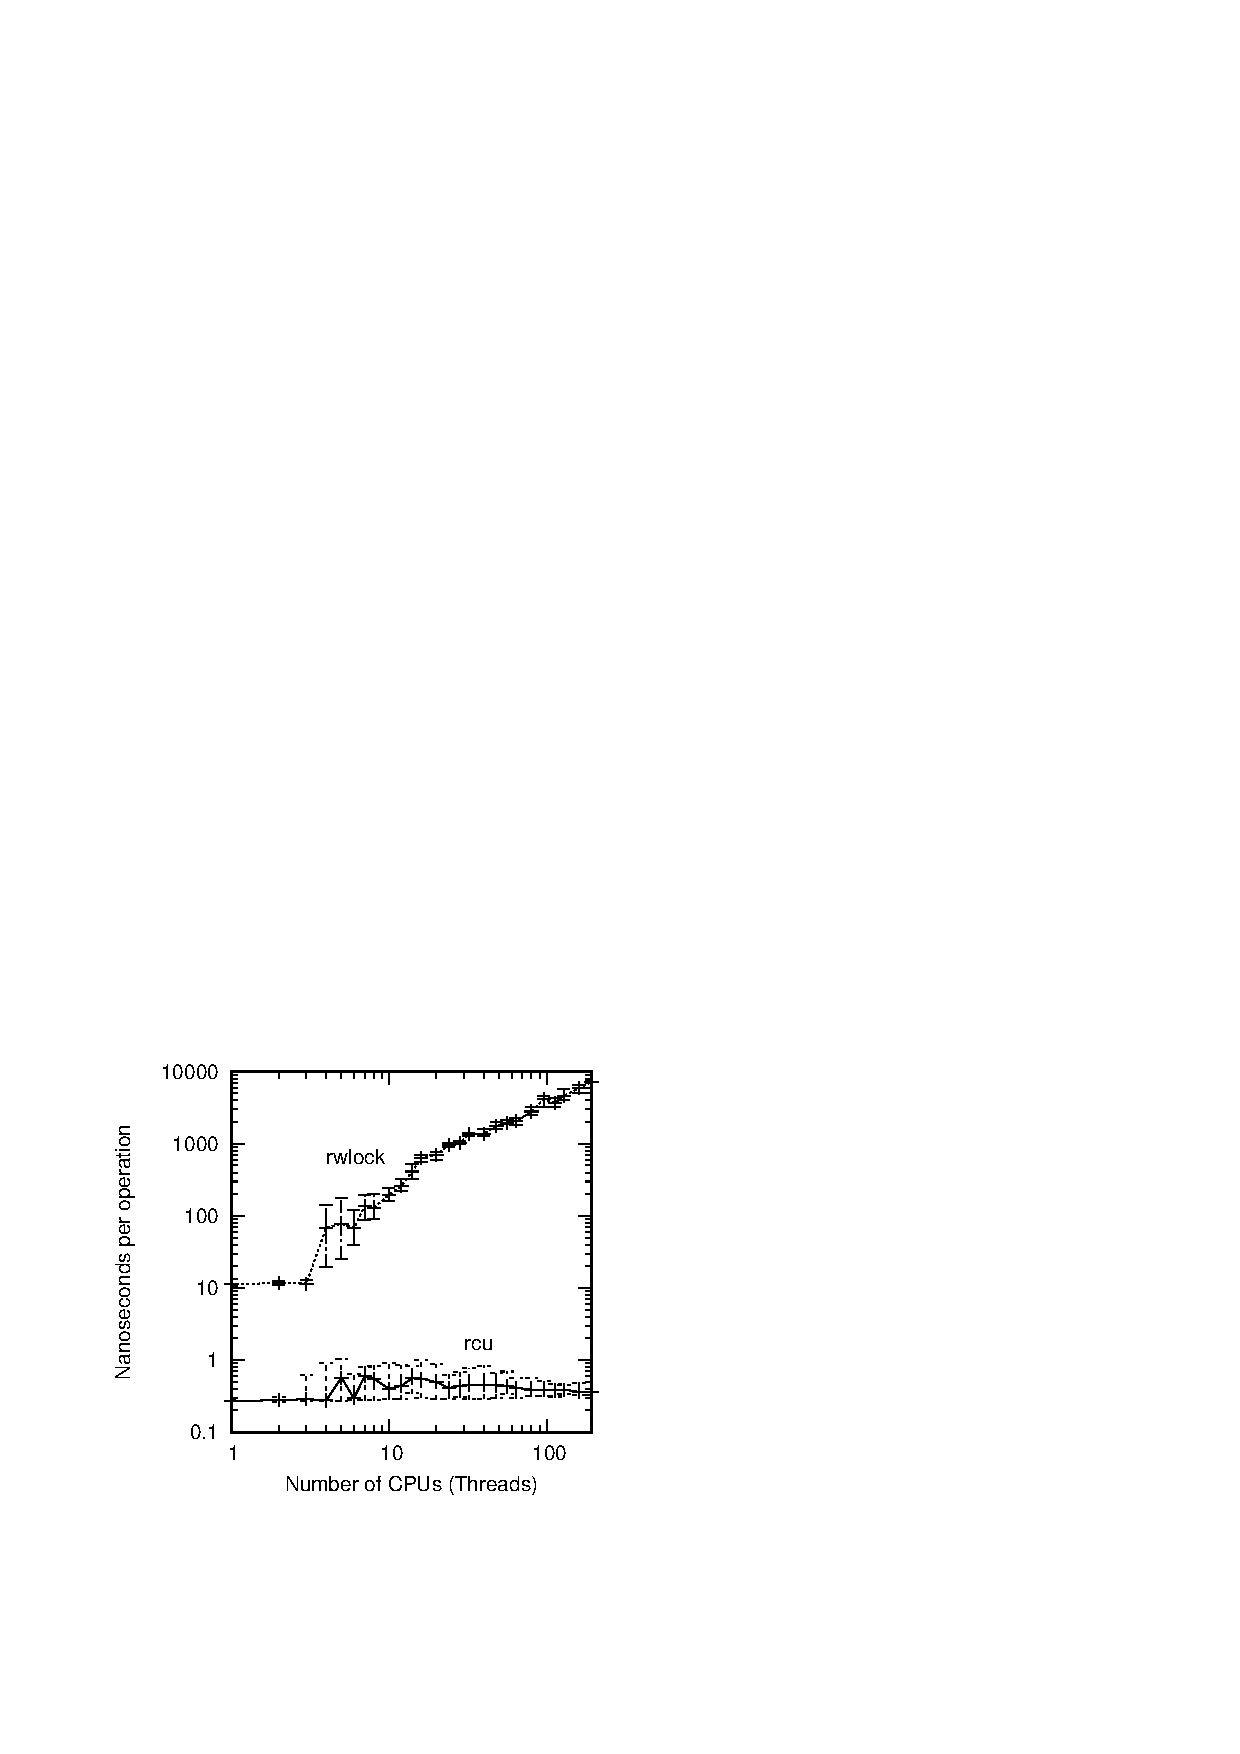
\includegraphics{CodeSamples/defer/data/rcuscale.hps.2020.05.28a/rwlockRCUperf}}
\caption{Performance Advantage of RCU Over Reader-Writer Locking}
\label{fig:defer:Performance Advantage of RCU Over Reader-Writer Locking}
\end{figure}

The read-side performance advantages of Linux-kernel RCU over
reader-writer locking are shown in
\cref{fig:defer:Performance Advantage of RCU Over Reader-Writer Locking},
which was generated on a 448-CPU 2.10\,GHz Intel x86 system.

\QuickQuizSeries{%
\QuickQuizB{
	WTF\@?
	How the heck do you expect me to believe that RCU can have less
	than a 300-picosecond overhead when the clock period at 2.10\,GHz
	is almost 500\,picoseconds?
}\QuickQuizAnswerB{
	First, consider that the inner loop used to
	take this measurement is as follows:

\begin{VerbatimN}
	for (i = nloops; i >= 0; i--) {
		rcu_read_lock();
		rcu_read_unlock();
	}
\end{VerbatimN}

	Next, consider the effective definitions of \co{rcu_read_lock()}
	and \co{rcu_read_unlock()}:

\begin{VerbatimN}
#define rcu_read_lock()   barrier()
#define rcu_read_unlock() barrier()
\end{VerbatimN}

	These definitions constrain compiler code-movement optimizations
	involving memory references, but emit no instructions in and
	of themselves.
	However, if the loop variable is maintained in a register,
	the accesses to \co{i} will not count as memory references.
	Furthermore, the compiler can do loop unrolling,
	allowing the resulting code to ``execute'' multiple passes
	through the loop body simply by incrementing \co{i} by
	some value larger than the value 1.

	So the ``measurement'' of 267 picoseconds is simply the fixed
	overhead of the timing measurements divided by the number of
	passes through the inner loop containing the calls
	to \co{rcu_read_lock()} and \co{rcu_read_unlock()}, plus
	the code to manipulate \co{i} divided by the loop-unrolling
	factor.
	And therefore, this measurement really is in error, in fact,
	it exaggerates the overhead by an arbitrary number of orders
	of magnitude.
	After all, in terms of machine instructions emitted, the actual
	overheads of \co{rcu_read_lock()} and of \co{rcu_read_unlock()}
	are each precisely zero.

	It is not just every day that a timing measurement of 267
	picoseconds turns out to be an overestimate!
}\QuickQuizEndB

\QuickQuizM{
	Didn't an earlier edition of this book show RCU read-side
	overhead way down in the sub-picosecond range?
	What happened???
}\QuickQuizAnswerM{
	Excellent memory!!!
	The overhead in some early releases was in fact roughly
	100~femtoseconds.

	What happened was that RCU usage spread more broadly through the
	Linux kernel, including into code that takes page faults.
	Back at that time, \co{rcu_read_lock()} and \co{rcu_read_unlock()}
	were complete no-ops in \co{CONFIG_PREEMPT=n} kernels.
	Unfortunately, that situation allowed the compiler to reorder
	page-faulting memory accesses into RCU read-side critical
	sections.
	Of course, page faults can block, which destroys those critical
	sections.

	Nor was this a theoretical problem:
	A failure actually manifested in 2019.
	\ppl{Herbert}{Xu} tracked down this failure and
	\ppl{Linus}{Torvalds}
	therefore queued a commit to upgrade \co{rcu_read_lock()} and
	\co{rcu_read_unlock()} to unconditionally include a call to
	\co{barrier()}~\cite{LinusTorvalds2019:RCUreader.barrier}.
	And although \co{barrier()} emits no code, it does constrain
	compiler optimizations.
	And so the price of widespread RCU usage is slightly higher
	\co{rcu_read_lock()} and \co{rcu_read_unlock()} overhead.
	As such, Linux-kernel RCU has proven to be a victim of its
	own success.

	Of course, it is also the case that the older results were obtained
	on a different system than were those shown in
	\cref{fig:defer:Performance Advantage of RCU Over Reader-Writer Locking}.
	So which change had the most effect, Linus's commit or the change in
	the system?
	This question is left as an exercise to the reader.
}\QuickQuizEndM

\QuickQuizE{
	Why is there such large variation for the \co{RCU} trace in
	\cref{fig:defer:Performance Advantage of RCU Over Reader-Writer Locking}?
}\QuickQuizAnswerE{
	Keep in mind that this is a log-log plot, so those large-seeming
	\co{RCU} variances in reality span only a few hundred picoseconds.
	And that is such a short time that anything could cause it.
	However, given that the variance decreases with both small and
	large numbers of CPUs, one hypothesis is that the variation is
	due to migrations from one CPU to another.

	Yes, these measurements were taken with interrupts disabled, but
	they were also taken within a guest OS, so that preemption was
	still possible at the hypervisor level.
	In addition, the system featured hyperthreading and a single
	hardware thread running this RCU workload is able to consume
	more than half of the core's resources.
	Therefore, the overall throughput varies depending on how many
	of a given guest OS's CPUs share cores.
	Attempting to reduce these variations by running the guest OSes
	at real-time priority (as suggested by Joel Fernandes) is left
	as an exercise for the reader.
}\QuickQuizEndE
}                 % End of \QuickQuizSeries

Note that reader-writer locking is more than an order of magnitude slower
than RCU on a single CPU, and is more than \emph{four} orders of magnitude
slower on 192~CPUs.
In contrast, RCU scales quite well.
In both cases, the error bars cover the full range of the measurements
from 30~runs, with the line being the median.

\begin{figure}
\centering
\resizebox{2.5in}{!}{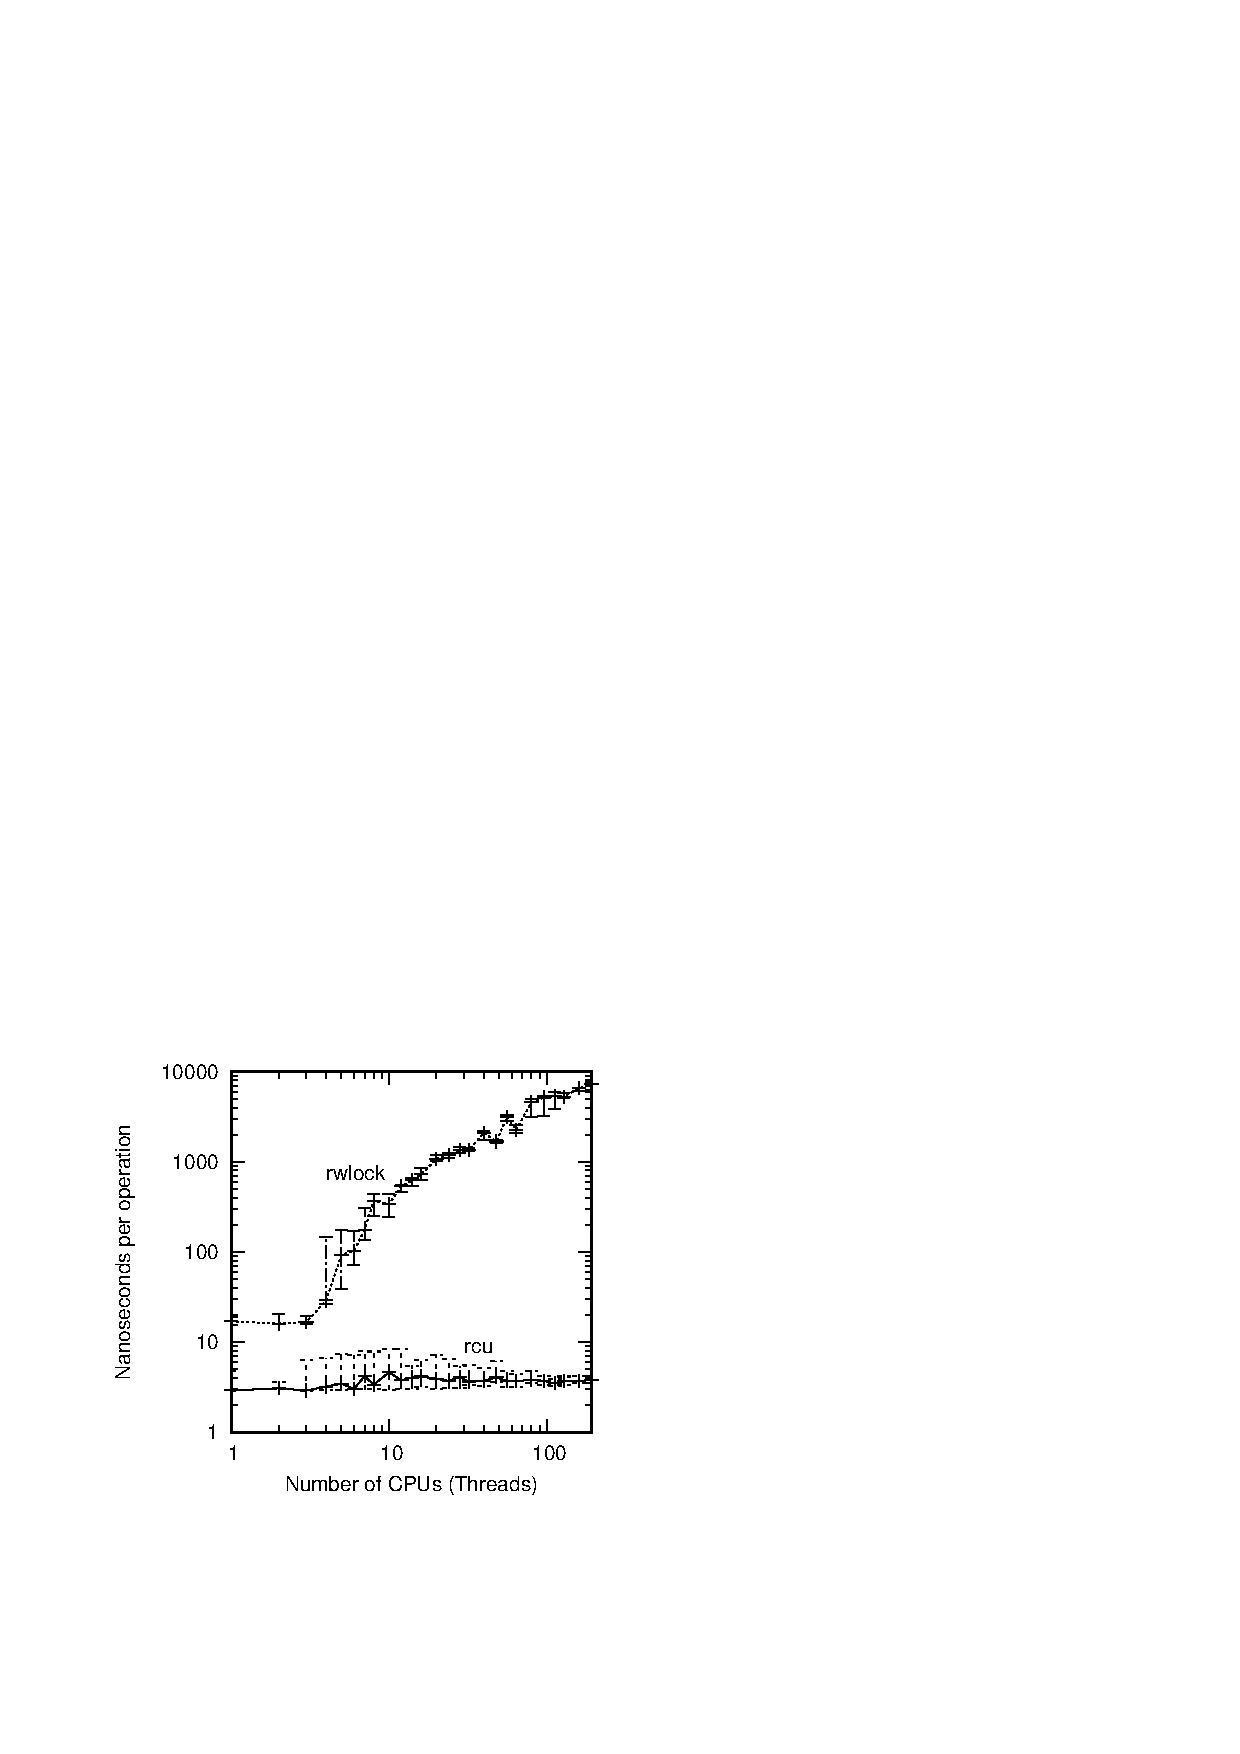
\includegraphics{CodeSamples/defer/data/rcuscale.hps.2020.05.28a/rwlockRCUperfPREEMPT}}
\caption{Performance Advantage of Preemptible RCU Over Reader-Writer Locking}
\label{fig:defer:Performance Advantage of Preemptible RCU Over Reader-Writer Locking}
\end{figure}

A more moderate view may be obtained from a \co{CONFIG_PREEMPT} kernel,
though RCU still beats reader-writer locking by between a factor of seven
on a single CPU and by three orders of magnitude on 192~CPUs, as shown in
\cref{fig:defer:Performance Advantage of Preemptible RCU Over Reader-Writer Locking},
which was generated on the same 448-CPU 2.10\,GHz x86 system.
Note the high variability of reader-writer locking at larger numbers of CPUs.
The error bars span the full range of data.

\QuickQuiz{
	Given that the system had no fewer than 448~hardware threads,
	why only 192~CPUs?
}\QuickQuizAnswer{
	Because the script (\path{rcuscale.sh}) that generates this data
	spawns a guest operating system for each set of points gathered,
	and on this particular system, both \co{qemu} and KVM limit the
	number of CPUs that may be configured into a given guest OS\@.
	Yes, it would have been possible to run a few more CPUs, but
	192 is a nice round number from a binary perspective, given
	that 256 is infeasible.
}\QuickQuizEnd

\begin{figure}
\centering
\resizebox{2.5in}{!}{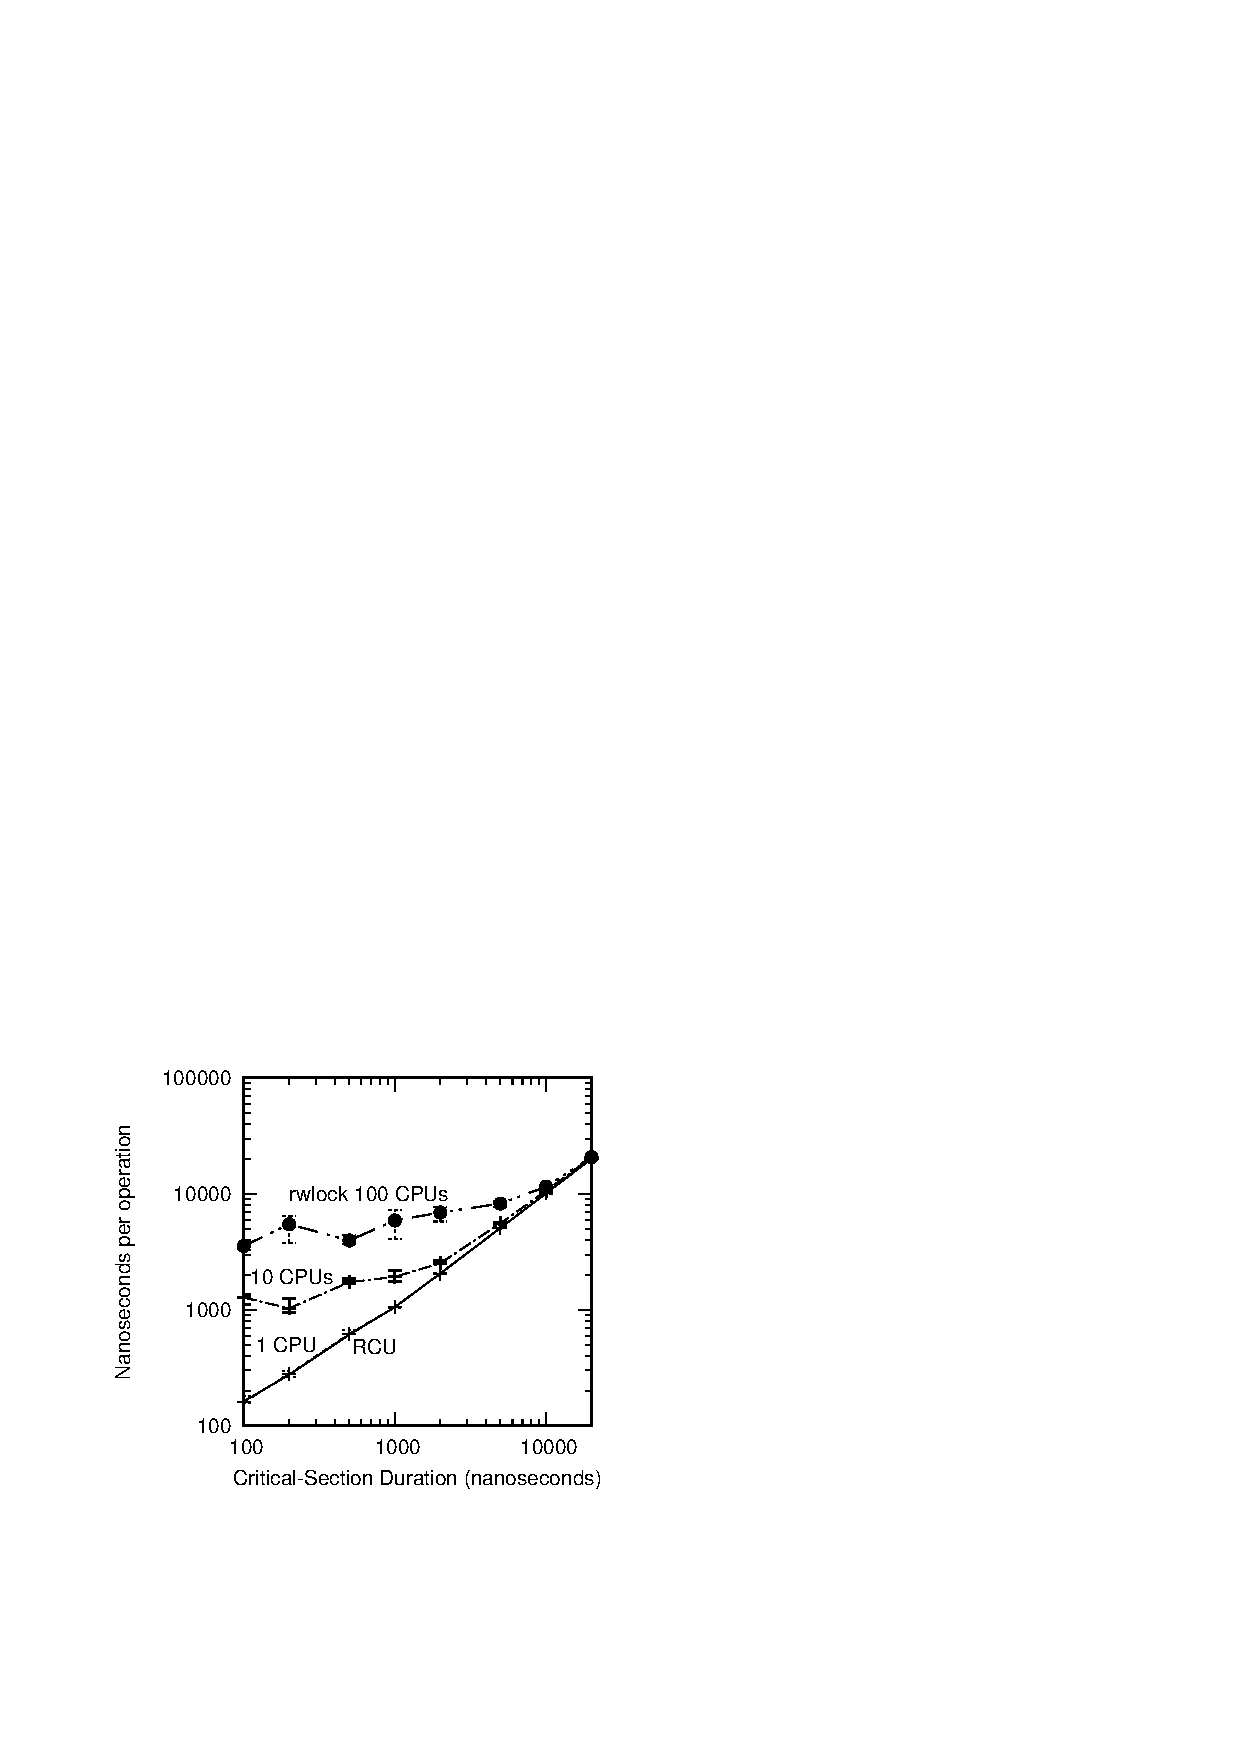
\includegraphics{CodeSamples/defer/data/rcuscale.hps.2020.05.28a/rwlockRCUperfwt}}
\caption{Comparison of RCU to Reader-Writer Locking as Function of Critical-Section Duration, 192 CPUs}
\label{fig:defer:Comparison of RCU to Reader-Writer Locking as Function of Critical-Section Duration}
\end{figure}

Of course, the low performance of reader-writer locking in
\cref{fig:defer:Performance Advantage of RCU Over Reader-Writer Locking,%
fig:defer:Performance Advantage of Preemptible RCU Over Reader-Writer Locking}
is exaggerated by the unrealistic zero-length critical sections.
The performance advantages of RCU decrease as the overhead of the critical
sections increase, as shown in
\cref{fig:defer:Comparison of RCU to Reader-Writer Locking as Function of Critical-Section Duration},
which was run on the same system as the previous plots.
Here, the y-axis represents the sum of the overhead of the read-side
primitives and that of the critical section and the x-axis represents
the critical-section overhead in nanoseconds.
But please note the logscale y~axis, which means that the small
separations between the traces still represent significant differences.
This figure shows non-preemptible RCU, but given that preemptible RCU's
read-side overhead is only about three nanoseconds, its plot would be
nearly identical to
\cref{fig:defer:Comparison of RCU to Reader-Writer Locking as Function of Critical-Section Duration}.

\QuickQuiz{
	Why the larger error ranges for the submicrosecond durations in
	\cref{fig:defer:Comparison of RCU to Reader-Writer Locking as Function of Critical-Section Duration}?
}\QuickQuizAnswer{
	Because smaller disturbances result in greater relative errors
	for smaller measurements.
	Also, the Linux kernel's \co{ndelay()} nanosecond-scale primitive
	is (as of 2020) less accurate than is the \co{udelay()} primitive
	used for the data for durations of a microsecond or more.
	It is instructive to compare to the zero-length case shown in
	\cref{fig:defer:Performance Advantage of RCU Over Reader-Writer Locking}.
}\QuickQuizEnd

There are three traces for reader-writer locking, with the upper trace
being for 100~CPUs, the next for 10~CPUs, and the lowest for 1~CPU\@.
The greater the number of CPUs and the shorter the critical sections,
the greater is RCU's performance advantage.
These performance advantages are underscored by the fact that 100-CPU
systems are no longer uncommon and that a number of system calls (and
thus any RCU read-side critical sections that they contain) complete
within microseconds.

In addition, as is discussed in the next paragraph,
RCU read-side primitives are almost entirely deadlock-immune.


\paragraph{Deadlock Immunity}

Although RCU offers significant performance advantages for
read-mostly workloads, one of the primary reasons for creating
RCU in the first place was in fact its immunity to read-side
deadlocks.
This immunity stems from the fact that
RCU read-side primitives do not block, spin, or even
do backwards branches, so that their execution time is deterministic.
It is therefore impossible for them to participate in a deadlock
cycle.

\QuickQuiz{
	Is there an exception to this deadlock immunity, and if so,
	what sequence of events could lead to deadlock?
}\QuickQuizAnswer{
	One way to cause a deadlock cycle involving
	RCU read-side primitives is via the following (illegal) sequence
	of statements:

\begin{VerbatimU}
rcu_read_lock();
synchronize_rcu();
rcu_read_unlock();
\end{VerbatimU}

	The \co{synchronize_rcu()} cannot return until all
	pre-existing RCU read-side critical sections complete, but
	is enclosed in an RCU read-side critical section that cannot
	complete until the \co{synchronize_rcu()} returns.
	The result is a classic self-deadlock---you get the same
	effect when attempting to write-acquire a reader-writer lock
	while read-holding it.

	Note that this self-deadlock scenario does not apply to
	RCU QSBR, because the context switch performed by the
	\co{synchronize_rcu()} would act as a quiescent state
	for this CPU, allowing a grace period to complete.
	However, this is if anything even worse, because data used
	by the RCU read-side critical section might be freed as a
	result of the grace period completing.
	Plus Linux kernel's lockdep facility will yell at you.

	In short, do not invoke synchronous RCU update-side primitives, which
	are listed in
	\cref{tab:defer:RCU Wait-to-Finish APIs},
	from within an RCU read-side critical section.

	In addition, within the Linux kernel, RCU uses the scheduler
	and the scheduler uses RCU\@.
	In some cases, both RCU and the scheduler must take care to
	avoid deadlock.
}\QuickQuizEnd

An interesting consequence of RCU's read-side deadlock immunity is
that it is possible to unconditionally upgrade an RCU
reader to an RCU updater.
Attempting to do such an upgrade with reader-writer locking results
in deadlock.
A sample code fragment that does an RCU read-to-update upgrade follows:

\begin{VerbatimN}[samepage=true]
rcu_read_lock();
list_for_each_entry_rcu(p, &head, list_field) {
	do_something_with(p);
	if (need_update(p)) {
		spin_lock(&my_lock);
		do_update(p);
		spin_unlock(&my_lock);
	}
}
rcu_read_unlock();
\end{VerbatimN}

Note that \co{do_update()} is executed under
the protection of the lock \emph{and} under RCU read-side protection.

Another interesting consequence of RCU's deadlock immunity is its
immunity to a large class of priority inversion problems.
For example, low-priority RCU readers cannot prevent a high-priority
RCU updater from acquiring the update-side lock.
Similarly, a low-priority RCU updater cannot prevent high-priority
RCU readers from entering an RCU read-side critical section.

\QuickQuiz{
	Immunity to both deadlock and priority inversion???
	Sounds too good to be true.
	Why should I believe that this is even possible?
}\QuickQuizAnswer{
	It really does work.
	After all, if it didn't work, the Linux kernel would not run.
}\QuickQuizEnd

\paragraph{Realtime Latency}

Because RCU read-side primitives neither spin nor block, they offer
excellent realtime latencies.
In addition, as noted earlier, this means that they are
immune to priority inversion
involving the RCU read-side primitives and locks.

However, RCU is susceptible to more subtle priority-inversion scenarios,
for example, a high-priority process blocked waiting for an RCU
grace period to elapse can be blocked by low-priority RCU readers
in \rt\ kernels.
This can be solved by using RCU priority
boosting~\cite{PaulEMcKenney2007BoostRCU,DinakarGuniguntala2008IBMSysJ}.

However, use of RCU priority boosting requires that \co{rcu_read_unlock()}
do deboosting, which entails acquiring scheduler locks.
Some care is therefore required within the scheduler and RCU to avoid
deadlocks, which as of the v5.15 Linux kernel requires RCU to avoid
invoking the scheduler while holding any of RCU's locks.

This in turn means that \co{rcu_read_unlock()} is not always lockless
when RCU priority boosting is enabled.
However, \co{rcu_read_unlock()} will still be lockless if its
critical section was not priority-boosted.
Furthermore, critical sections will not be priority boosted unless they
are preempted, or, in -rt kernels, they acquire non-raw spinlocks.
This means that \co{rcu_read_unlock()} will normally be lockless from the
perspective of the highest priority task running on any given CPU.

\paragraph{RCU Readers and Updaters Run Concurrently}

Because RCU readers never spin nor block, and because updaters are not
subject to any sort of rollback or abort semantics, RCU readers and
updaters really can run concurrently.
This means that RCU readers might access stale data, and might even
see inconsistencies, either of which can render conversion from reader-writer
locking to RCU non-trivial.

\begin{figure}
\centering
\resizebox{3in}{!}{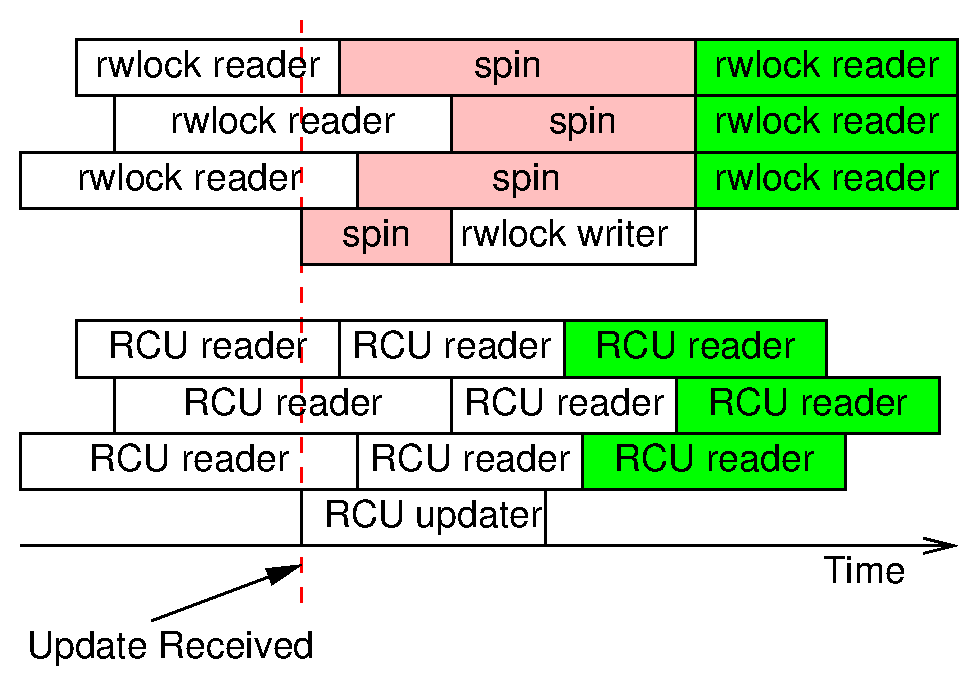
\includegraphics{defer/rwlockRCUupdate}}
\caption{Response Time of RCU vs.\@ Reader-Writer Locking}
\label{fig:defer:Response Time of RCU vs. Reader-Writer Locking}
\end{figure}

However, in a surprisingly large number of situations, inconsistencies and
stale data are not problems.
The classic example is the networking routing table.
Because routing updates can take considerable time to reach a given
system (seconds or even minutes), the system will have been sending
packets the wrong way for quite some time when the update arrives.
It is usually not a problem to continue sending updates the wrong
way for a few additional milliseconds.
Furthermore, because RCU updaters can make changes without waiting for
RCU readers to finish,
the RCU readers might well see the change more quickly than would
batch-fair
reader-writer-locking readers, as shown in
\cref{fig:defer:Response Time of RCU vs. Reader-Writer Locking}.
This faster RCU response time has since been corroborated (if perhaps
a bit unrealistically) by Markov-model
analysis~\cite[Figures 3 and 5]{VishakhaRamani2023LockBasedLocklessFresh}.

\QuickQuiz{
	But how many other algorithms really tolerate stale and
	inconsistent data?
}\QuickQuizAnswer{
	Quite a few!

	Please keep in mind that the finite speed of light means that
	data reaching a given computer system is at least slightly stale
	at the time that it arrives, and extremely stale in the case
	of astronomical data.
	The finite speed of light also places a sharp limit on the
	consistency of data arriving from different sources or via
	different paths.

	You might as well face the fact that the laws of physics
	are incompatible with naive notions of perfect freshness and
	consistency.
}\QuickQuizEnd

Once the update is received, the rwlock writer cannot proceed until the
last reader completes, and subsequent readers cannot proceed until the
writer completes.
However, these subsequent readers are guaranteed to see the new value,
as indicated by the green shading of the rightmost boxes.
In contrast, RCU readers and updaters do not block each other, which permits
the RCU readers to see the updated values sooner.
Of course, because their execution overlaps that of the RCU updater,
\emph{all} of the RCU readers might well see updated values, including
the three readers that started before the update.
Nevertheless only the green-shaded rightmost RCU readers
are \emph{guaranteed} to see the updated values.

Reader-writer locking and RCU simply provide different guarantees.
With reader-writer locking, any reader that begins after the writer begins
is guaranteed to see new values, and any reader that attempts to
begin while the writer is spinning might or might not see new values,
depending on the reader/writer preference of the rwlock implementation in
question.
In contrast, with RCU, any reader that begins after the updater completes
is guaranteed to see new values, and any reader that completes after the
updater begins might or might not see new values, depending on timing.

The key point here is that, although reader-writer locking does
indeed guarantee consistency within the confines of the computer system,
there are situations where this consistency comes at the price of
increased \emph{inconsistency} with the outside world, courtesy of
the finite speed of light and the non-zero size of atoms.
In other words, reader-writer locking obtains internal consistency at the
price of silently stale data with respect to the outside world.

Note that if a value is computed while read-holding a reader-writer
lock, and then that value is used after that lock is released, then
this reader-writer-locking use case is using stale data.
After all, the quantities that this value is based on could change
at any time after that lock is released.
This sort of reader-writer-locking use case is often easy to
convert to RCU, as will be shown in
\cref{lst:defer:Converting Reader-Writer Locking to RCU: Data,%
lst:defer:Converting Reader-Writer Locking to RCU: Search,%
lst:defer:Converting Reader-Writer Locking to RCU: Deletion}
and the accompanying text.

\paragraph{Low-Priority RCU Readers Can Block High-Priority Reclaimers}

In Realtime RCU~\cite{DinakarGuniguntala2008IBMSysJ} or
SRCU~\cite{PaulEMcKenney2006c},
a preempted reader will prevent a grace period from completing, even if
a high-priority task is blocked waiting for that grace period to complete.
Realtime RCU can avoid this problem by substituting \co{call_rcu()}
for \co{synchronize_rcu()} or by using RCU priority
boosting~\cite{PaulEMcKenney2007BoostRCU,DinakarGuniguntala2008IBMSysJ}.
It might someday be necessary to augment SRCU and RCU Tasks Trace with
priority boosting, but not before a clear real-world need is demonstrated.

\QuickQuiz{
	If Tasks RCU Trace might someday be priority boosted, why
	not also Tasks RCU and Tasks RCU Rude?
}\QuickQuizAnswer{
	Maybe, but these are less likely.

	In the case of Tasks RCU, recall that the quiescent state is
	a voluntary context switch.
	Thus, all tasks not blocked after a voluntary context switch
	might need to be boosted, and the mechanics of deboosting would
	not likely be at all pretty.

	In the case of Tasks RCU Rude, as was the case with the old
	RCU Sched, any preemptible region of code is a quiescent state.
	Thus, the only tasks that might need boosting are those currently
	running with preemption disabled.
	But boosting the priority of a preemption-disabled task has no
	effect.
	It therefore seems doubly unlikely that priority boosting will
	ever be introduced to Tasks RCU Rude, at least in its current
	form.
}\QuickQuizEnd

\paragraph{RCU Grace Periods Extend for Many Milliseconds}

With the exception of userspace
RCU~\cite{MathieuDesnoyers2009URCU,PaulMcKenney2013LWNURCU},
expedited grace periods, and several of the ``toy''
RCU implementations described in
\cref{chp:app:``Toy'' RCU Implementations},
RCU grace periods extend milliseconds.
Although there are a number of techniques to render such long
delays harmless, including use of the asynchronous interfaces
(\co{call_rcu()} and \co{call_rcu_bh()}) or of the polling interfaces
(\co{get_state_synchronize_rcu()}, \co{start_poll_synchronize_rcu()},
and \co{poll_state_synchronize_rcu()}), this situation is a major reason
for the rule of thumb that RCU be used in read-mostly situations.

As noted in \cref{sec:defer:RCU Linux-Kernel API}, within the Linux
kernel, shorter grace periods may be obtained via expedited grace
periods, for example, by invoking \co{synchronize_rcu_expedited()}
instead of \co{synchronize_rcu()}.
Expedited grace periods can reduce delays to as little as a few tens of
microseconds, albeit at the expense of higher CPU utilization and IPIs.
The added IPIs can be especially unwelcome in some real-time workloads.

\paragraph{Code:
		 Reader-Writer Locking vs.\@ RCU}

In the best case, the conversion from reader-writer locking to RCU
is quite simple, as shown in
\cref{lst:defer:Converting Reader-Writer Locking to RCU: Data,%
lst:defer:Converting Reader-Writer Locking to RCU: Search,%
lst:defer:Converting Reader-Writer Locking to RCU: Deletion},
all taken from
Wikipedia~\cite{WikipediaRCU}.

\begin{listing*}
{ \scriptsize
\begin{verbbox}
 1 struct el {                           1 struct el {
 2   struct list_head lp;                2   struct list_head lp;
 3   long key;                           3   long key;
 4   spinlock_t mutex;                   4   spinlock_t mutex;
 5   int data;                           5   int data;
 6   /* Other data fields */             6   /* Other data fields */
 7 };                                    7 };
 8 DEFINE_RWLOCK(listmutex);             8 DEFINE_SPINLOCK(listmutex);
 9 LIST_HEAD(head);                      9 LIST_HEAD(head);
\end{verbbox}
}
\hspace*{0.9in}\OneColumnHSpace{-0.5in}
\IfEbookSize{\hspace*{-1.05in}}{}\theverbbox
\caption{Converting Reader-Writer Locking to RCU\@:
						    Data}
\label{lst:defer:Converting Reader-Writer Locking to RCU: Data}
\end{listing*}

\begin{listing*}
{ \scriptsize
\begin{verbbox}
 1 int search(long key, int *result)     1 int search(long key, int *result)
 2 {                                     2 {
 3   struct el *p;                       3   struct el *p;
 4                                       4
 5   read_lock(&listmutex);              5   rcu_read_lock();
 6   list_for_each_entry(p, &head, lp) { 6   list_for_each_entry_rcu(p, &head, lp) {
 7     if (p->key == key) {              7     if (p->key == key) {
 8       *result = p->data;              8       *result = p->data;
 9       read_unlock(&listmutex);        9       rcu_read_unlock();
10       return 1;                      10       return 1;
11     }                                11     }
12   }                                  12   }
13   read_unlock(&listmutex);           13   rcu_read_unlock();
14   return 0;                          14   return 0;
15 }                                    15 }
\end{verbbox}
}
\hspace*{0.9in}\OneColumnHSpace{-0.5in}
\IfEbookSize{\hspace*{-1.05in}}{}\theverbbox
\caption{Converting Reader-Writer Locking to RCU\@:
						    Search}
\label{lst:defer:Converting Reader-Writer Locking to RCU: Search}
\end{listing*}

\begin{listing*}
{ \scriptsize
\begin{verbbox}
 1 int delete(long key)                  1 int delete(long key)
 2 {                                     2 {
 3   struct el *p;                       3   struct el *p;
 4                                       4
 5   write_lock(&listmutex);             5   spin_lock(&listmutex);
 6   list_for_each_entry(p, &head, lp) { 6   list_for_each_entry(p, &head, lp) {
 7     if (p->key == key) {              7     if (p->key == key) {
 8       list_del(&p->lp);               8       list_del_rcu(&p->lp);
 9       write_unlock(&listmutex);       9       spin_unlock(&listmutex);
                                        10       synchronize_rcu();
10       kfree(p);                      11       kfree(p);
11       return 1;                      12       return 1;
12     }                                13     }
13   }                                  14   }
14   write_unlock(&listmutex);          15   spin_unlock(&listmutex);
15   return 0;                          16   return 0;
16 }                                    17 }
\end{verbbox}
}
\hspace*{0.9in}\OneColumnHSpace{-0.5in}
\IfEbookSize{\hspace*{-1.05in}}{}\theverbbox
\caption{Converting Reader-Writer Locking to RCU\@:
						    Deletion}
\label{lst:defer:Converting Reader-Writer Locking to RCU: Deletion}
\end{listing*}

However, the transformation is not always this straightforward.
This is because neither the \co{spin_lock()} nor the
\co{synchronize_rcu()} in
\cref{lst:defer:Converting Reader-Writer Locking to RCU: Deletion}
exclude the readers in
\cref{lst:defer:Converting Reader-Writer Locking to RCU: Search}.
First, the \co{spin_lock()} does not interact in any way with
\co{rcu_read_lock()} and \co{rcu_read_unlock()}, thus not excluding them.
Second, although both \co{write_lock()} and \co{synchronize_rcu()}
wait for pre-existing readers, only \co{write_lock()} prevents
subsequent readers from commencing.\footnote{
	Kudos to whoever pointed this out to Paul.}
Thus, \co{synchronize_rcu()} cannot exclude readers.
Nevertheless, a great many situations using reader-writer locking can
be converted to RCU\@.

More-elaborate cases of replacing reader-writer locking with RCU
may be found
elsewhere~\cite{NeilBrown2015PathnameLookup,NeilBrown2015RCUwalk}.

\paragraph{Semantics:
		      Reader-Writer Locking vs.\@ RCU}

Expanding on the previous section, reader-writer locking semantics can
be roughly and informally summarized by the following three temporal
constraints:

\begin{enumerate}
\item	Write-side acquisitions wait for any read-holders to release
	the lock.
\item	Write-side acquisitions wait for any write-holder to release
	the lock.
\item	Read-side acquisitions wait for any write-holder to release
	the lock.
\end{enumerate}

RCU dispenses entirely with constraint~\#3 and weakens the other two
as follows:

\begin{enumerate}
\item	Writers wait for any pre-existing read-holders before progressing
	to the destructive phase of their update (usually the freeing of
	memory).
\item	Writers synchronize with each other as needed.
\end{enumerate}

It is of course this weakening that permits RCU implementations to attain
excellent performance and scalability.
It also allows RCU to implement the aforementioned unconditional
read-to-write upgrade that is so attractive and so deadlock-prone in
reader-writer locking.
Code using RCU can compensate for this weakening in a surprisingly large
number of ways, but most commonly by imposing spatial constraints:

\begin{enumerate}
\item	New data is placed in newly allocated memory.
\item	Old data is freed, but only after:
	\begin{enumerate}
	\item	That data has been unlinked so as to be inaccessible
		to later readers, and
	\item	A subsequent RCU grace period has elapsed.
	\end{enumerate}
\end{enumerate}

Of course, there are some reader-writer-locking use cases for which
RCU's weakened semantics are inappropriate, but experience in the Linux
kernel indicates that more than 80\pct\ of reader-writer locks can in fact
be replaced by RCU\@.
For example, a common reader-writer-locking use case computes some value
while holding the lock and then uses that value after releasing that lock.
This use case results in stale data, and therefore often accommodates
RCU's weaker semantics.

\begin{listing}
\input{CodeSamples/defer/singleton@get.fcv}
\caption{RCU Singleton Get}
\label{lst:defer:Singleton Get}
\end{listing}

\begin{listing}
\input{CodeSamples/defer/singleton@set.fcv}
\caption{RCU Singleton Set}
\label{lst:defer:Singleton Set}
\end{listing}

\begin{fcvref}[ln:defer:singleton:get]
This interaction of temporal and spatial constraints is illustrated
by the RCU singleton data structure illustrated in
\cref{fig:defer:Insertion With Concurrent Readers,fig:defer:Deletion With Concurrent Readers}.
This structure is defined on \clnrefrange{myconfig.b}{myconfig.e} of
\cref{lst:defer:Singleton Get}, and contains two integer fields,
\co{->a} and \co{->b} (\path{singleton.c}).
The current instance of this structure is referenced by the \co{curconfig}
pointer defined on \clnref{myconfig.e}.
\end{fcvref}

\begin{fcvref}[ln:defer:singleton:get]
The fields of the current structure are passed back through the
\co{cur_a} and \co{cur_b} parameters to the \co{get_config()} function
defined on \clnrefrange{get_config.b}{get_config.e}.
These two fields can be slightly out of date, but they absolutely must
be consistent with each other.
The \co{get_config()} function provides this consistency
within the RCU read-side critical section starting on
\clnref{rrl} and ending on either \clnref{rrul1} or \clnref{rrul2},
which provides the needed temporal synchronization.
\Clnref{rderef} fetches the pointer to the current \co{myconfig} structure.
This structure will be used regardless of any concurrent changes due
to calls to the \co{set_config()} function, thus providing the needed
spatial synchronization.
If \clnref{nullchk} determines that the \co{curconfig} pointer was
\co{NULL}, \clnref{retfail} returns failure.
Otherwise, \clnref{copya,copyb} copy out the \co{->a} and \co{->b} fields
and \clnref{retsuccess} returns success.
These \co{->a} and \co{->b} fields are from the same \co{myconfig}
structure, and the RCU read-side critical section prevents this structure
from being freed, thus guaranteeing that these two fields are consistent
with each other.
\end{fcvref}

\begin{fcvref}[ln:defer:singleton:set]
The structure is updated by the \co{set_config()} function shown in
\cref{lst:defer:Singleton Set}.
\Clnrefrange{allocinit.b}{allocinit.e} allocate and initialize a
new \co{myconfig} structure.
\Clnref{xchg} atomically exchanges a pointer to this new structure with
the pointer to the old structure in \co{curconfig}, while also providing
full memory ordering both before and after the \co{xchg()} operation,
thus providing the needed updater/reader spatial synchronization on
the one hand and the needed updater/updater synchronization on the other.
If \clnref{if} determines that the pointer to the old structure was
in fact non-\co{NULL}, \clnref{sr} waits for a grace period (thus providing
the needed reader/updater temporal synchronization) and \clnref{free}
frees the old structure, safe in the knowledge that there are no
longer any readers still referencing it.
\end{fcvref}

\begin{figure*}
\centering
\resizebox{\onecolumntextwidth}{!}{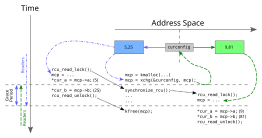
\includegraphics{defer/RCUspacetime}}
\caption{RCU Spatial/Temporal Synchronization}
\label{fig:defer:RCU Spatial/Temporal Synchronization}
\end{figure*}

\Cref{fig:defer:RCU Spatial/Temporal Synchronization} shows an abbreviated
representation of \co{get_config()} on the left and right and a similarly
abbreviated representation of \co{set_config()} in the middle.
Time advances from top to bottom, and the address space of the objects
referenced by \co{curconfig} advances from left to right.
The boxes with comma-separated numbers each represent a \co{myconfig}
structure, with the constraint that \co{->b} is the square of \co{->a}.
Each blue dash-dotted arrow represents an interaction with the old structure
(on the left, containing ``5,25'') and each green dashed arrow represents
an interaction with the new structure (on the right, containing ``9,81'').

The black dotted arrows represent temporal relationships between RCU readers
on the left and right and the RCU grace period at center, with each
arrow pointing from an older event to a newer event.
The call to \co{synchronize_rcu()} followed the leftmost \co{rcu_read_lock()},
and therefore that \co{synchronize_rcu()} invocation must not return
until after the corresponding \co{rcu_read_unlock()}.
In contrast, the call to \co{synchronize_rcu()} precedes the
rightmost \co{rcu_read_lock()}, which allows the return from that same
\co{synchronize_rcu()} to ignore the corresponding \co{rcu_read_unlock()}.
These temporal relationships prevent the \co{myconfig} structures from
being freed while RCU readers are still accessing them.

The two horizontal grey dashed lines represent the period of time during
which different readers get different results, however, each reader
will see one and only one of the two objects.
All readers that end before the first horizontal line will see the
leftmost \co{myconfig} structure, and all readers that start after the
second horizontal line will see the rightmost structure.
Between the two lines, that is, during the grace period, different
readers might see different objects, but as long as each reader
loads the \co{curconfig} pointer only once, each reader will see
a consistent view of its \co{myconfig} structure.

\QuickQuiz{
	But doesn't the RCU grace period start sometime after the
	call to \co{synchronize_rcu()} rather than in the middle
	of that \co{xchg()} statement?
}\QuickQuizAnswer{
	Which grace period, exactly?

	The updater is required to wait for at least one grace
	period that starts at or some time after the removal,
	in this case, the \co{xchg()}.
	So in
	\cref{fig:defer:RCU Spatial/Temporal Synchronization},
	the indicated grace period starts as early as theoretically
	possible and extends to the return from \co{synchronize_rcu()}.
	This is a perfectly legal grace period corresponding to the
	change carried out by that \co{xchg()} statement.
}\QuickQuizEnd

In short, when operating on a suitable linked data structure, RCU
combines temporal and spatial synchronization in order to approximate
reader-writer locking, with RCU read-side critical sections acting as
the reader-writer-locking reader, as shown in
\cref{fig:defer:Relationships Between RCU Use Cases,fig:defer:RCU Spatial/Temporal Synchronization}.
RCU's temporal synchronization is provided by the read-side markers,
for example, \co{rcu_read_lock()} and \co{rcu_read_unlock()}, as well as
the update-side grace-period primitives, for example, \co{synchronize_rcu()}
or \co{call_rcu()}.
The spatial synchronization is provided by the read-side
\co{rcu_dereference()} family of primitives, each of which subscribes
to a version published by \co{rcu_assign_pointer()}.\footnote{
	Preferably with both \co{rcu_dereference()} and
	\co{rcu_assign_pointer()} being embedded in higher-level APIs.}
RCU's combining of temporal and spatial synchronization contrasts to
the schemes presented in
\cref{sec:SMPdesign:Code Locking,sec:SMPdesign:Data Locking,sec:locking:Inefficiency},
in which temporal and spatial synchronization are provided separately by
locking and by static data-structure layout, respectively.

\QuickQuiz{
	Is RCU the only synchronization mechanism that combines temporal
	and spatial synchronization in this way?
}\QuickQuizAnswer{
	Not at all.

	Hazard pointers can be considered to combine temporal and spatial
	synchronization in a similar manner.
	Referring to
	\cref{lst:defer:Hazard-Pointer Recording and Clearing},
	the \co{hp_record()} function's acquisition of a reference
	provides both spatial and temporal synchronization, subscribing
	to a version and marking the start of a reference, respectively.
	This function therefore combines the effects of RCU's
	\co{rcu_read_lock()} and \co{rcu_dereference()}.
	Referring now to
	\cref{lst:defer:Hazard-Pointer Scanning and Freeing},
	the \co{hp_clear()} function's release of a reference provides
	temporal synchronization marking the end of a reference, and is
	thus similar to RCU's \co{rcu_read_unlock()}.
	The \co{hazptr_free_later()} function's retiring of a
	hazard-pointer-protected object provides temporal synchronization,
	similar to RCU's \co{call_rcu()}.
	The primitives used to mutate a hazard-pointer-protected
	structure provide spatial synchronization, similar to RCU's
	\co{rcu_assign_pointer()}.

	Alternatively, one could instead come at hazard pointers by
	analogy with reference counting.
	And, by doing so, learn that reference counting also combines
	temporal and spatial synchronization as described above for
	hazard pointers.
}\QuickQuizEnd

\subsubsection{Quasi Reference Count}
\label{sec:defer:Quasi Reference Count}

Because grace periods are not allowed to complete while
there is an RCU read-side critical section in progress,
the RCU read-side primitives may be used as a restricted
reference-counting mechanism.
For example, consider the following code fragment:

\begin{VerbatimN}
rcu_read_lock();  /* acquire reference. */
p = rcu_dereference(head);
/* do something with p. */
rcu_read_unlock();  /* release reference. */
\end{VerbatimN}

The combination of the \co{rcu_read_lock()} and \co{rcu_dereference()}
primitives can be thought of as acquiring a reference to \co{p},
because a grace period starting after the \co{rcu_dereference()}
assignment to \co{p} cannot possibly end until after we reach the matching
\co{rcu_read_unlock()}.
This reference-counting scheme is restricted in that it is forbidden
to wait for RCU grace periods within RCU read-side critical sections,
and also forbidden to hand off an RCU read-side critical section's
references from one task to another.

Regardless of these restrictions,
the following code can safely delete \co{p}:

\begin{VerbatimN}
spin_lock(&mylock);
p = head;
rcu_assign_pointer(head, NULL);
spin_unlock(&mylock);
/* Wait for all references to be released. */
synchronize_rcu();
kfree(p);
\end{VerbatimN}

The assignment to \co{head} prevents any future references
to \co{p} from being acquired, and the \co{synchronize_rcu()}
waits for any previously acquired references to be released.

\QuickQuiz{
	But wait!
	This is exactly the same code that might be used when thinking
	of RCU as a replacement for reader-writer locking!
	What gives?
}\QuickQuizAnswer{
	This is an effect of the Law of Toy Examples:
	Beyond a certain point, the code fragments look the same.
	The only difference is in how we think about the code.
	For example, what does an \co{atomic_inc()} operation do?
	It might be acquiring another explicit reference to an object
	to which we already have a reference, it might be incrementing
	an often-read/seldom-updated statistical counter, it might
	be checking into an HPC-style barrier, or any of a number of
	other things.

	However, these differences can be extremely important.
	For but one example of the importance, consider that if we think
	of RCU as a restricted reference counting scheme, we would never
	be fooled into thinking that the updates would exclude the RCU
	read-side critical sections.

	It nevertheless is often useful to think of RCU as a replacement
	for reader-writer locking, for example, when you are replacing
	reader-writer locking with RCU\@.
}\QuickQuizEnd

Of course, RCU can also be combined with traditional reference counting,
as discussed in
\cref{sec:together:Refurbish Reference Counting}.

\begin{figure}
\centering
\resizebox{2.5in}{!}{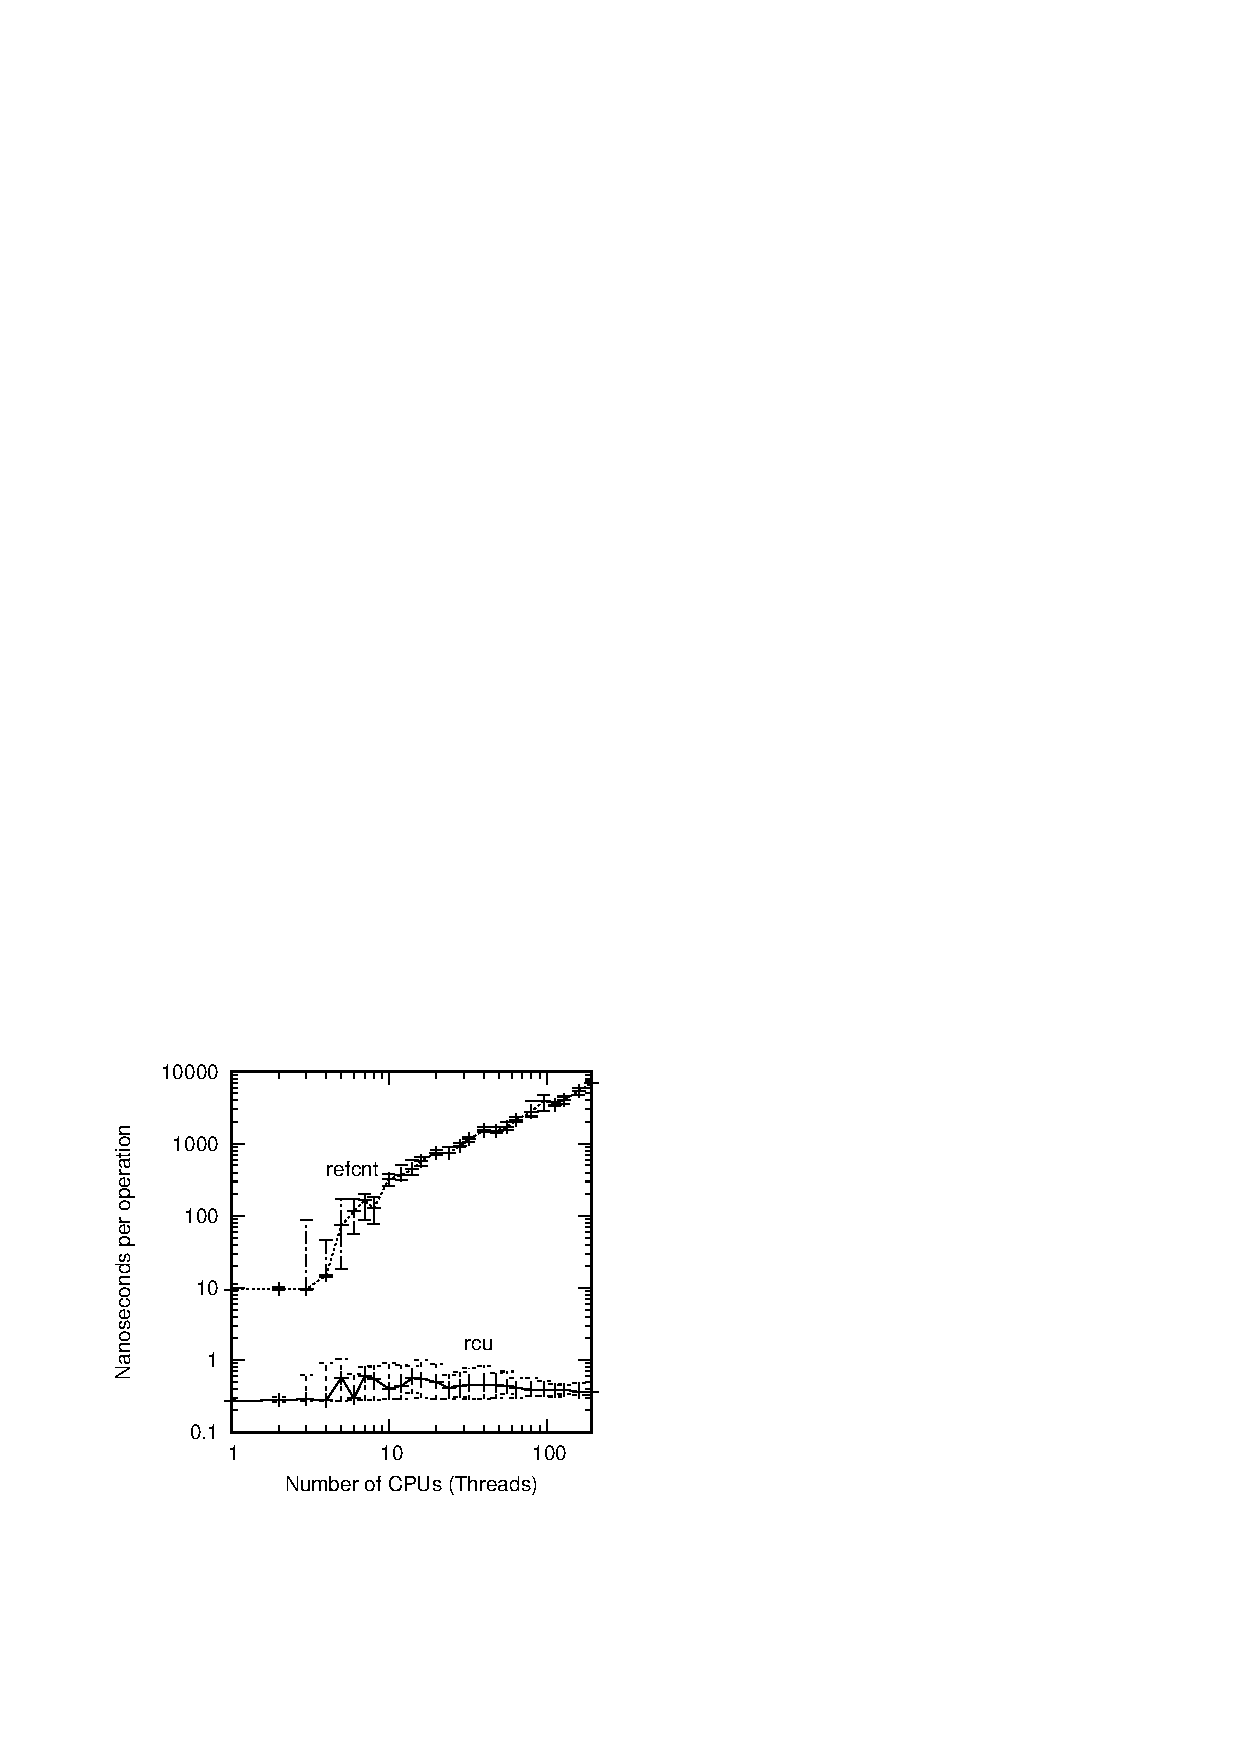
\includegraphics{CodeSamples/defer/data/rcuscale.hps.2020.05.28a/refcntRCUperf}}
\caption{Performance of RCU vs.\@ Reference Counting}
\label{fig:defer:Performance of RCU vs. Reference Counting}
\end{figure}

\begin{figure}
\centering
\resizebox{2.5in}{!}{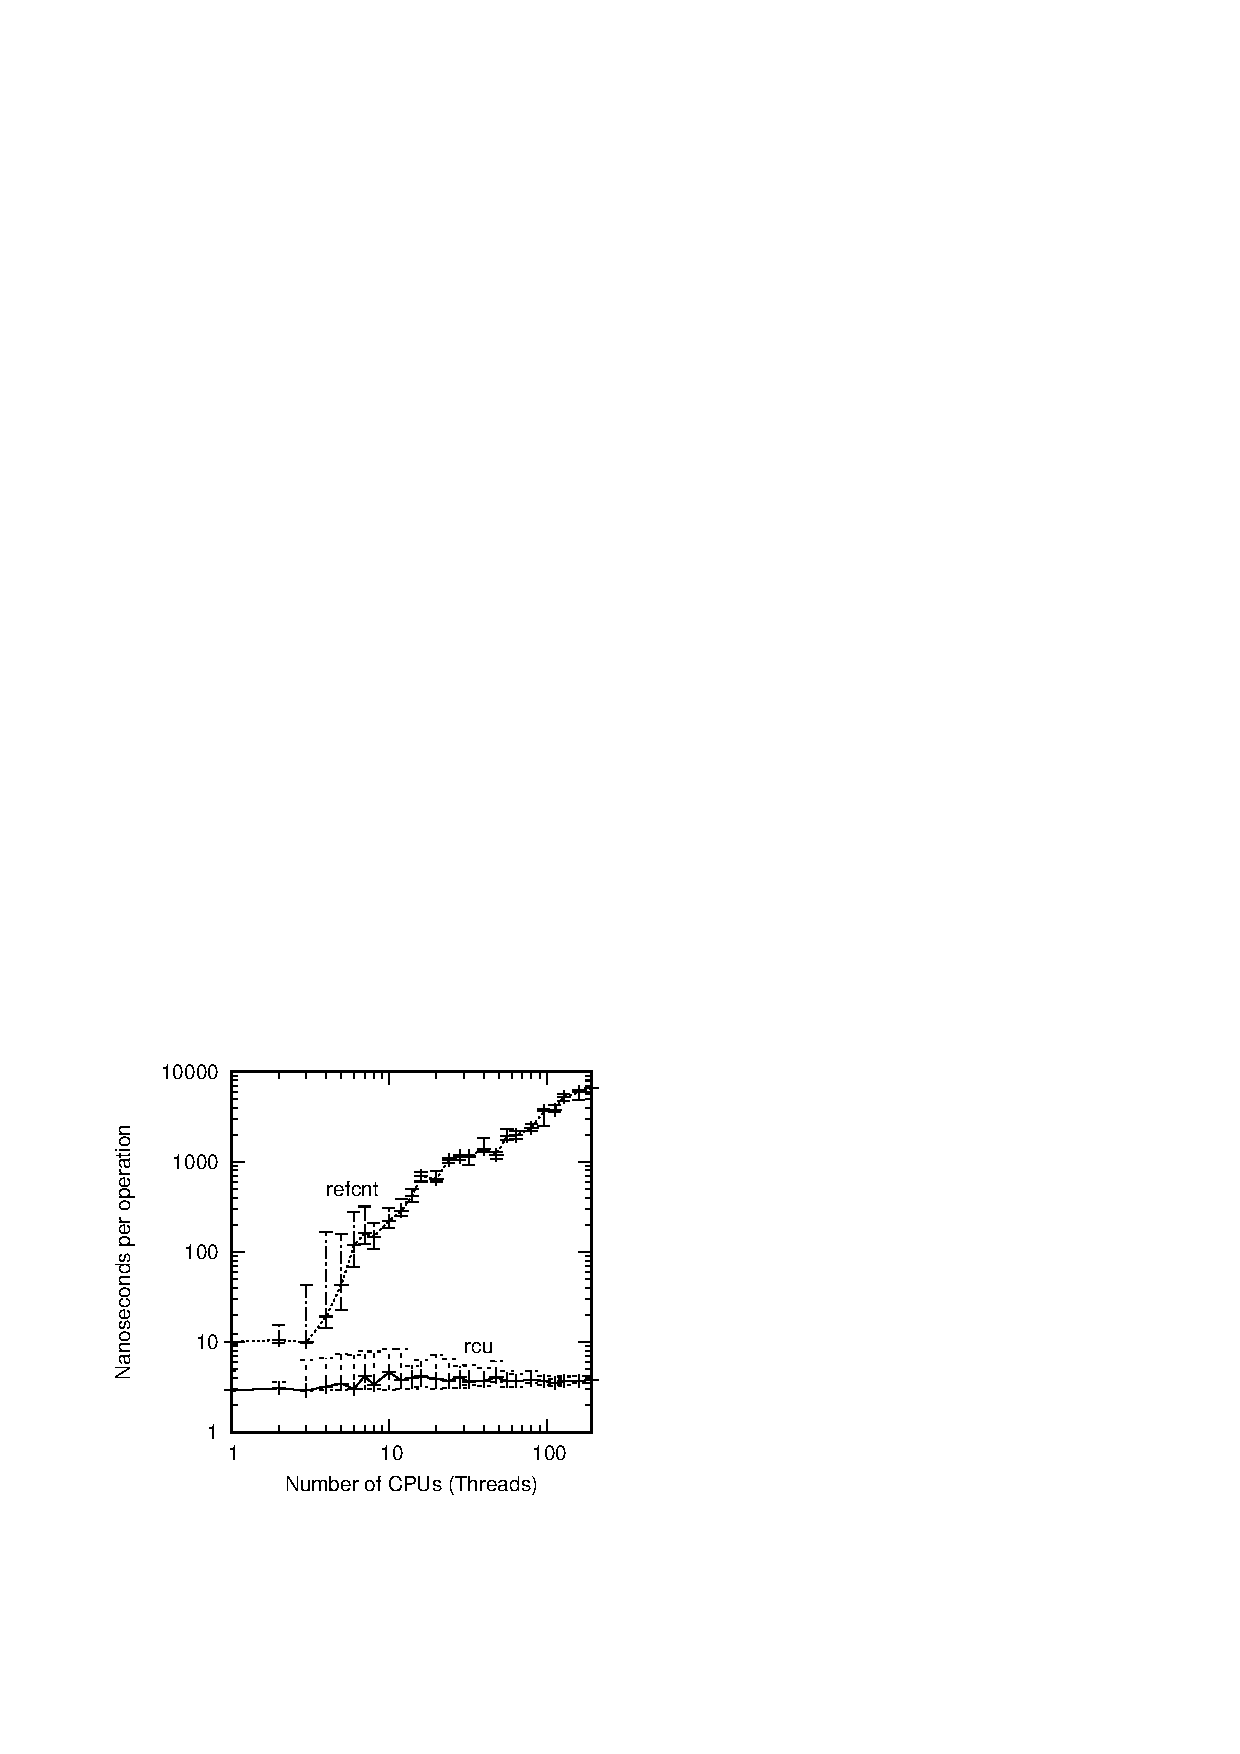
\includegraphics{CodeSamples/defer/data/rcuscale.hps.2020.05.28a/refRCUperfPREEMPT}}
\caption{Performance of Preemptible RCU vs.\@ Reference Counting}
\label{fig:defer:Performance of Preemptible RCU vs. Reference Counting}
\end{figure}

But why bother?
Again, part of the answer is performance, as shown in
\cref{fig:defer:Performance of RCU vs. Reference Counting,%
fig:defer:Performance of Preemptible RCU vs. Reference Counting},
again showing data taken on a 448-CPU 2.1\,GHz Intel x86 system
for non-preemptible and preemptible Linux-kernel RCU, respectively.
Non-preemptible RCU's advantage over
\IXalt{reference counting}{reference count} ranges from
more than an order of magnitude at one CPU up to about four orders of
magnitude at 192~CPUs.
Preemptible RCU's advantage ranges from about a factor of three at
one CPU up to about three orders of magnitude at 192~CPUs.

\begin{figure}
\centering
\resizebox{2.5in}{!}{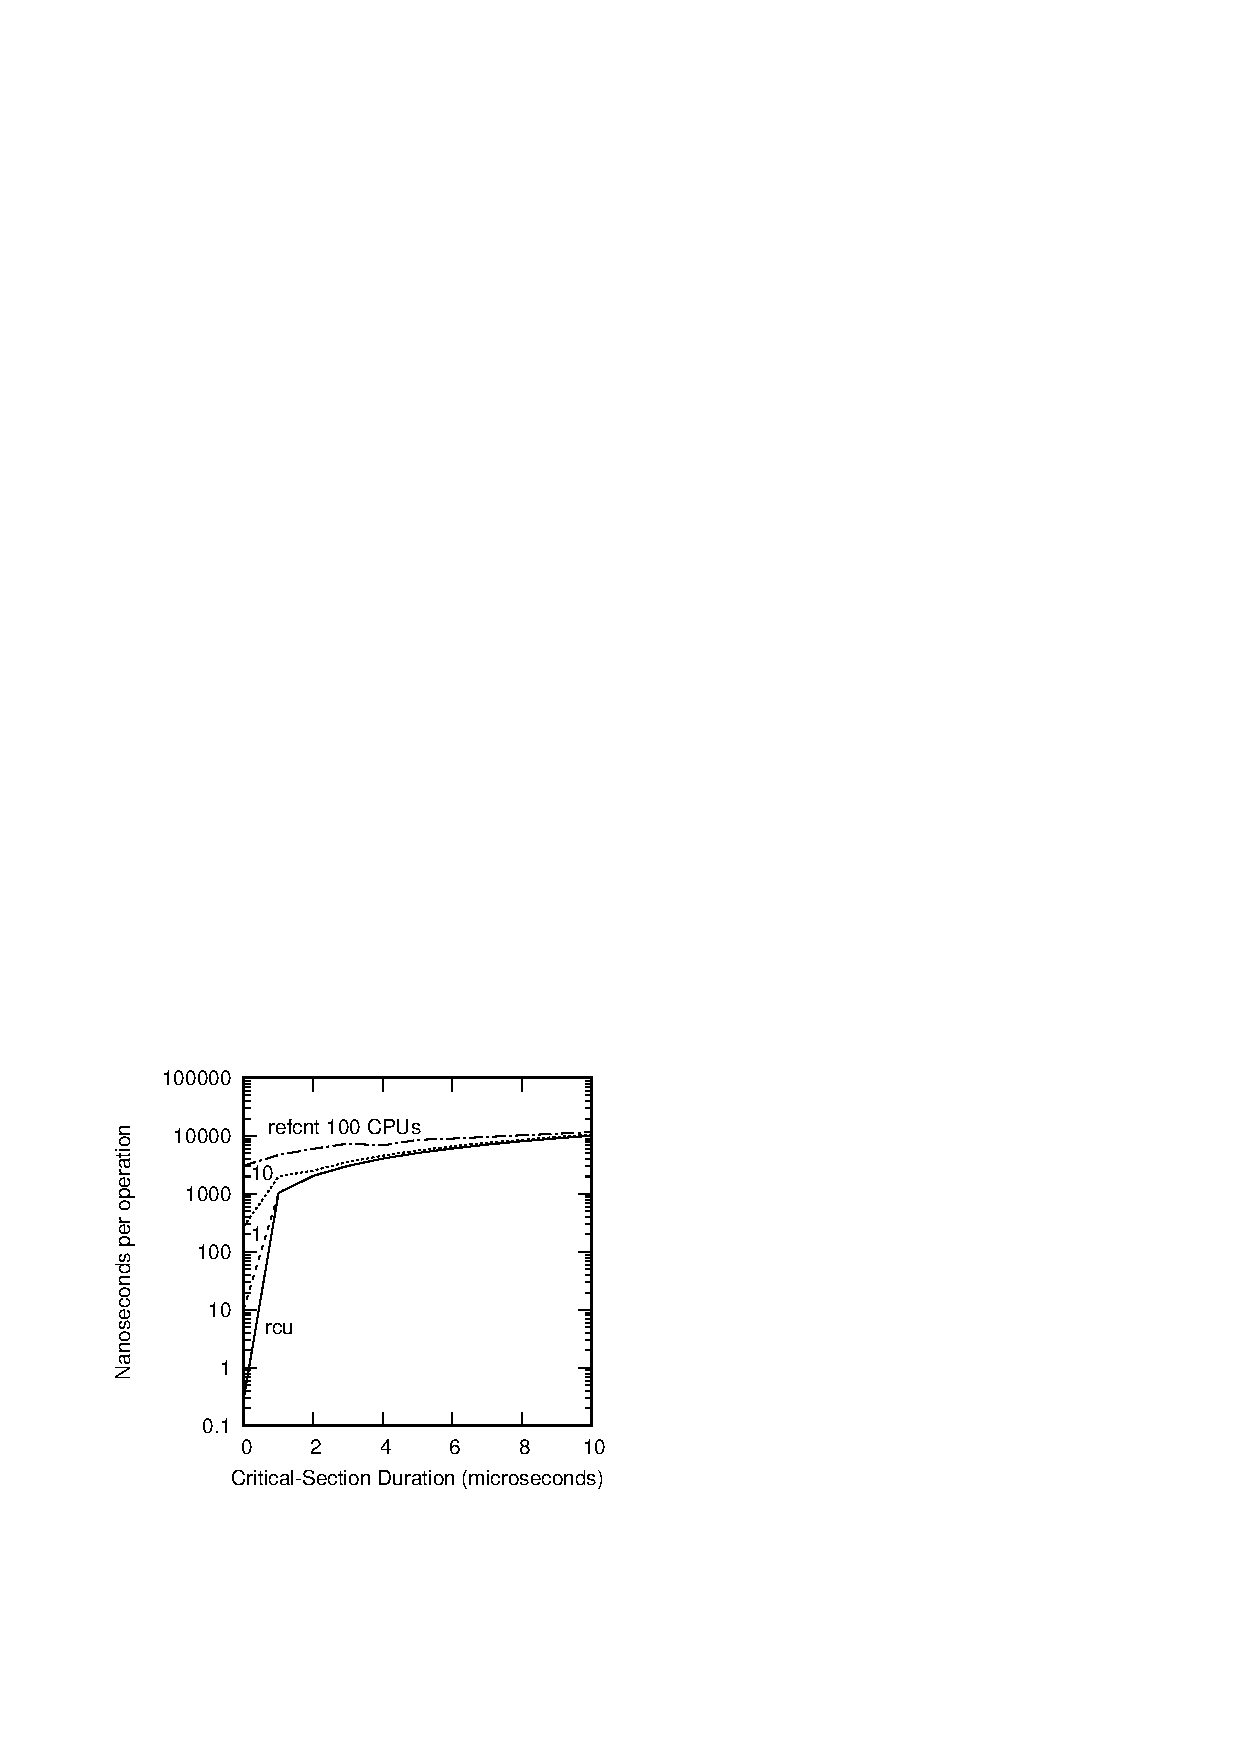
\includegraphics{CodeSamples/defer/data/rcuscale.hps.2020.05.28a/refRCUperfwt}}
\caption{Response Time of RCU vs.\@ Reference Counting, 192 CPUs}
\label{fig:defer:Response Time of RCU vs. Reference Counting}
\end{figure}

However, as with reader-writer locking, the performance advantages of
RCU are most pronounced for short-duration critical sections and for
large numbers of CPUs, as shown in
\cref{fig:defer:Response Time of RCU vs. Reference Counting}
for the same system.
In addition, as with reader-writer locking, many system calls (and thus
any RCU read-side critical sections that they contain) complete in
a few microseconds.

Although traditional reference counters are usually associated with a
specific data structure, or perhaps a specific group of data structures,
this approach does have some disadvantages.
For example, maintaining a single global reference counter for a large
variety of data structures typically results in bouncing the cache line
containing the reference count.
As we saw in
\crefrange{fig:defer:Performance of RCU vs. Reference Counting}{fig:defer:Response Time of RCU vs. Reference Counting},
such cache-line bouncing can severely degrade performance.

In contrast, RCU's lightweight \co{rcu_read_lock()},
\co{rcu_dereference()}, and \co{rcu_read_unlock()} read-side primitives
permit extremely frequent read-side usage with negligible performance
degradation.
Except that the calls to \co{rcu_dereference()} are not doing anything
specific to acquire a reference to the pointed-to object.
The heavy lifting is instead done by the \co{rcu_read_lock()} and
\co{rcu_read_unlock()} primitives and their interactions with RCU
grace periods.

And ignoring those calls to \co{rcu_dereference()} permits RCU to be
thought of as a ``bulk reference-counting'' mechanism, where each call
to \co{rcu_read_lock()} obtains a reference on each and every RCU-protected
object, and with little or no overhead.
However, the restrictions that go with RCU can be quite onerous.
For example, in many cases, the Linux-kernel prohibition against
sleeping while in an RCU read-side critical section would defeat the
entire purpose.
Such cases might be better served by the hazard pointers mechanism
described in \cref{sec:defer:Hazard Pointers}.
Cases where code rarely sleeps have been handled by using RCU as a
reference count in the common non-sleeping case and by bridging
to an explicit reference counter when sleeping is necessary.

Alternatively, situations where a reference must be held by a single task
across a section of code that sleeps may be accommodated with Sleepable
RCU (SRCU)~\cite{PaulEMcKenney2006c}.
This fails to cover the not-uncommon situation where a reference is ``passed''
from one task to another, for example, when a reference is acquired
when starting an I/O and released in the corresponding completion
interrupt handler.
Again, such cases might be better handled by explicit reference counters
or by hazard pointers.

Of course, SRCU brings restrictions of its own, namely that the
return value from \co{srcu_read_lock()} be passed into the
corresponding \co{srcu_read_unlock()}, and that no SRCU primitives
be invoked from hardware interrupt handlers or from \IXacrf{nmi}
handlers.
The jury is still out as to how much of a problem is presented by
this restriction, and as to how it can best be handled.

However, in the common case where references are held within the confines
of a single CPU or task, RCU can be used as a high-performance and highly
scalable reference-counting mechanism.

As shown in \cref{fig:defer:Relationships Between RCU Use Cases},
quasi reference counts add RCU readers as individual or bulk
reference counts, possibly also bridging to reference counters
in corner cases.

\subsubsection{Quasi Multi-Version Concurrency Control}
\label{sec:defer:Quasi Multi-Version Concurrency Control}

RCU can also be thought of as a simplified multi-version concurrency
control (MVCC) mechanism with weak consistency criteria.
The multi-version aspects were touched upon in
\cref{sec:defer:Maintain Multiple Versions of Recently Updated Objects}.
However, in its native form, RCU provides version consistency only
within a given RCU-protected data element.

Nevertheless, there are situations where consistency and fresh data are
required across multiple data elements.
Fortunately, there are a number of approaches that avoid inconsistency
and stale data, including the following:

\begin{enumerate}
\item	Enclose RCU readers within sequence-locking readers, forcing
	the RCU readers to be retried should an update occur,
	as described in
	\cref{sec:together:Correlated Data Elements}
	and
	\cref{sec:together:Atomic Move}.
\item	Place the data that must be consistent into a single element
	of a linked data structure, and refrain from updating those
	fields within any element visible to RCU readers.
	RCU readers gaining a reference to any such element are then
	guaranteed to see consistent values.
	See \cref{sec:together:Correlated Fields} for additional details.
\item	Use a per-element lock that guards a ``deleted'' flag to allow
	RCU readers to reject stale
	data~\cite{PaulEdwardMcKenneyPhD,Arcangeli03}
	as detailed in
	\cref{sec:together:Fresh and Consistent Data}.
\item	Provide an existence flag that is referenced by all data elements
	whose update is to appear atomic to RCU
	readers~\cite{PaulEMcKennneyAtomicTreeN4037,PaulEMcKennneyAtomicTreeCPPCON2014,PaulEMcKenneyIssaquahUpdate2015,PaulEMcKenney2016IssaquahACMApp,PaulEMcKenney2016IssaquahCPPCON}.
\item	Use one of a wide range of counter-based
	methods~\cite{PaulEMcKenney2008cyclicRCU,PaulEMcKenney2010cyclicRCU,PaulEMcKenney2011cyclicparallelRCU,PaulEMcKenney2014cyclicRCU,Matveev:2015:RLS:2815400.2815406,Kim:2019:MSR:3297858.3304040}.
	In these approaches, updaters maintain a version number and maintain links
	to old versions of a given piece of data.
	Readers take a snapshot of the current version number, and, if necessary,
	traverse the links to find a version consistent with that snapshot.
\end{enumerate}

In short, when using RCU to approximate multi-version concurrency control,
you only pay for the level of consistency that you actually need.

As shown in \cref{fig:defer:Relationships Between RCU Use Cases},
quasi multi-version concurrency control is based on existence guarantees,
adding read-side snapshot operations and constraints on readers and
writers, the exact form of the constraint being dictated by the
consistency requirements, as summarized above.

\subsubsection{RCU Usage Summary}
\label{sec:defer:RCU Usage Summary}

At its core, RCU is nothing more nor less than an API that provides:

\begin{enumerate}
\item	A publish-subscribe mechanism for adding new data,
\item	A way of waiting for pre-existing RCU readers to finish, and
\item	A discipline of maintaining multiple versions to permit change
	without harming or unduly delaying concurrent RCU readers.
\end{enumerate}

That said, it is possible to build higher-level constructs on top of RCU,
including the various use cases described in the earlier sections.
Furthermore, I have no doubt that new use cases will continue to be
found for RCU, as well as for any of a number of other synchronization
primitives.
And so it is that RCU's use cases are conceptually more complex than
is RCU itself, as hinted on
\cpageref{sec:defer:Mysteries RCU Use Cases}.

\QuickQuiz{
	Which of these use cases best describes the Pre-BSD routing
	example in
	\cref{sec:defer:RCU for Pre-BSD Routing}?
}\QuickQuizAnswer{
	Pre-BSD routing could be argued to fit into either
	quasi reader-writer lock, quasi reference count, or
	quasi multi-version concurrency control.
	The code is the same either way.
	This is similar to things like \co{atomic_inc()}, another tool
	that can be put to a great many uses.
}\QuickQuizEnd

\begin{figure}
\centering
\resizebox{3in}{!}{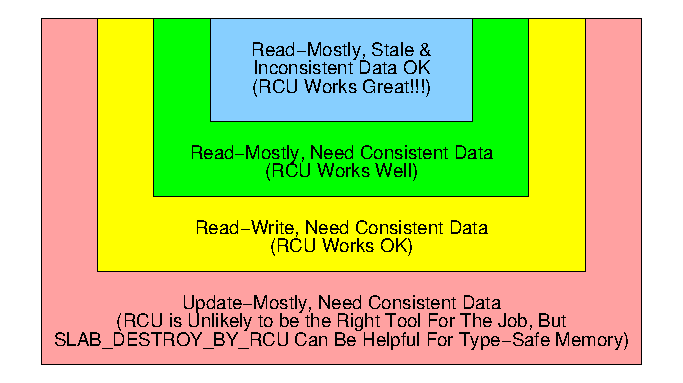
\includegraphics{defer/RCUApplicability}}
\caption{RCU Areas of Applicability}
\label{fig:defer:RCU Areas of Applicability}
\end{figure}

In the meantime,
\cref{fig:defer:RCU Areas of Applicability}
shows some rough rules of thumb on where RCU is most helpful.

As shown in the blue box in the upper-right corner of the figure, RCU
works best if you have read-mostly data where stale and inconsistent
data is permissible (but see below for more information on stale and
inconsistent data).
The canonical example of this case in the Linux kernel is routing tables.
Because it may have taken many seconds or even minutes for the
routing updates to propagate across the Internet, the system
has been sending packets the wrong way for quite some time.
Having some small probability of continuing to send some of them the wrong
way for a few more milliseconds is almost never a problem.

If you have a read-mostly workload where consistent data is required,
RCU works well, as shown by the green ``read-mostly, need consistent data''
box.
One example of this case is the Linux kernel's mapping from user-level
System-V semaphore IDs to the corresponding in-kernel data structures.
Semaphores tend to be used far more frequently than they are created
and destroyed, so this mapping is read-mostly.
However, it would be erroneous to perform a semaphore operation on
a semaphore that has already been deleted.
This need for consistency is handled by using the lock in the
in-kernel semaphore data structure, along with a ``deleted''
flag that is set when deleting a semaphore.
If a user ID maps to an in-kernel data structure with the
``deleted'' flag set, the data structure is ignored, so that
the user ID is flagged as invalid.

Although this requires that the readers acquire a lock for the
data structure representing the semaphore itself,
it allows them to dispense with locking for the
mapping data structure.
The readers therefore locklessly
traverse the tree used to map from ID to data structure,
which in turn greatly improves performance, scalability, and
real-time response.

As indicated by the yellow ``read-write'' box, RCU can also be useful
for read-write
workloads where consistent data is required, although usually in
conjunction with a number of other synchronization primitives.
For example, the directory-entry cache in recent Linux kernels uses RCU in
conjunction with sequence locks, per-CPU locks, and per-data-structure
locks to allow lockless traversal of pathnames in the common case.
Although RCU can be very beneficial in this read-write case, the
corresponding code is often more complex than that of the read-mostly
cases.

Finally, as indicated by the red box in the lower-left corner
of the figure, update-mostly workloads requiring consistent
data are rarely good places to use RCU, though there are some
exceptions~\cite{MathieuDesnoyers2012URCU}.
For example, as noted in
\cref{sec:defer:Type-Safe Memory},
within the Linux kernel, the \co{SLAB_TYPESAFE_BY_RCU}
slab-allocator flag provides type-safe memory to RCU readers, which can
greatly simplify \IXacrl{nbs} and other lockless
algorithms.
In addition, if the rare readers are on critical code paths on real-time
systems, use of RCU for those readers might provide real-time response
benefits that more than make up for the increased update-side overhead,
as discussed in \cref{sec:advsync:The Role of RCU}.

In short, RCU is an API that includes a publish-subscribe mechanism for
adding new data, a way of waiting for pre-existing RCU readers to finish,
and a discipline of maintaining multiple versions to allow updates to
avoid harming or unduly delaying concurrent RCU readers.
This RCU API is best suited for read-mostly situations, especially if
stale and inconsistent data can be tolerated by the application.

% defer/rcurelated.tex
% mainfile: ../perfbook.tex
% SPDX-License-Identifier: CC-BY-SA-3.0

\subsection{RCU Related Work}
\label{sec:defer:RCU Related Work}
\OriginallyPublished{sec:defer:RCU Related Work}{RCU Related Work}{Linux Weekly News}{PaulEMcKenney2014ReadMostly}
\OriginallyPublished{sec:defer:RCU Related Work}{RCU Related Work}{Linux Weekly News}{PaulEMcKenney2015ReadMostly}

The first known mention of anything resembling RCU took the form of a bug
report from
\ppl{Donald}{Knuth}~\cite[page 413 of Fundamental Algorithms]{Knuth73}
against \ppl{Joseph}{Weizenbaum}'s SLIP list-processing facility for
FORTRAN~\cite{Weizenbaum:1963:SLP:367593.367617}.
Knuth was justified in reporting the bug, as SLIP had no notion of
any sort of grace-period guarantee.

The first known non-bug-report mention of anything resembling RCU appeared
in \pplsur{H. T.}{Kung}'s and \pplsur{Philip L.}{Lehman}'s landmark
paper~\cite{Kung80}.
There was some additional use of this technique in
academia~\cite{Manber82,Manber84,BarbaraLiskov1988ArgusCACM,Pugh90,Andrews91textbook,Pu95a,Cowan96a,Rastogi:1997:LPV:645923.671017,Gamsa99},
but much of the work in this area was instead carried out by
practitioners~\cite{RichardRashid87a,Hennessy89,Jacobson93,AjuJohn95,Slingwine95,Slingwine97,Slingwine98,McKenney98}.

\QuickQuiz{
	Garbage collectors?
	Passive serialization?
	System reference points?
	Quiescent states?
	Aging?
	Generations?
	Why on earth couldn't the knuckleheads working on these early
	papers bring themselves to agree on a common terminology???
}\QuickQuizAnswer{
	There were multiple independent inventions of mechanisms
	vaguely resembling RCU\@.
	Each group of inventors was unaware of the others, so each
	made up its own terminology as a matter of course.
	And the different terminology made it quite difficult for
	any one group to find any of the others.

	Sorry, but life is like that sometimes!
}\QuickQuizEnd

By the year 2000, the initiative had passed to open-source projects,
most notably the Linux kernel
community~\cite{RustyRussell2000a,RustyRussell2000b,McKenney01b,McKenney01a,McKenney02a,Arcangeli03}.\footnote{
	A list of citations with well over 200 entries may be found in
	\co{bib/RCU.bib} in the {\LaTeX} source for this book.}
RCU was accepted into the Linux kernel in late 2002, with many subsequent
improvements for scalability, robustness, real-time response, energy
efficiency, and specialized use cases.
As of 2023, Linux-kernel RCU is still under active development.

\QuickQuiz{
	Why didn't Kung's and Lehman's paper result in immediate use
	of RCU?
}\QuickQuizAnswer{
	One reason is that Kung and Lehman were simply ahead of their
	time.
	Another reason was that their approach, ground-breaking though
	it was, did not take a number of software-engineering and
	performance issues into account.

	To see that they were ahead of their time, consider that three
	years after their paper was published, Paul was working on a
	PDP-11 system running BSD 2.8.
	This system lacked any sort of automatic configuration, which
	meant that any hardware modification, including adding a new
	disk drive, required hand-editing and rebuilding the kernel.
	Furthermore, this was a single-CPU system, which meant that
	full-system synchronization was a simple matter of disabling
	interrupts.

	Fast-forward a number of years, and multicore systems permitting
	runtime changes in hardware configuration were commonplace.
	This meant that the hardware configuration data that was implicitly
	represented in 1980s kernel source code was now a mutable
	data structure that was accessed on every I/O\@.
	Such data structures rarely change, but could change at any time.
	And this read-mostly property applies to many other new-age
	data structures, including those concerning networking (rare in
	the 1980s), security policies (physical locks in the 1980s),
	software configuration (immutable at runtime in the 1980s),
	and much else besides.
	There was thus much more opportunity for RCU to demonstrate its
	benefits in the 1990s and 2000s than there was in the 1980s.

	Kung's and Lehman's software-engineering sins included failing
	to mark readers (thus presenting debugging difficulties),
	failing to provide a clean RCU API (thus tying their mechanism
	to a specific data structure), and failing to allow for any
	post-grace-period operation other than freeing memory (thus
	disallowing a number of RCU use cases).

	Kung and Lehman presented two garbage-collection strategies.
	The first waited for all processes running at a given time
	to terminate, which represented another software-engineering
	sin that ruled out their mechanism's use in software that
	runs indefinitely.
	The second used per-object reference counting, which greatly
	complicates their read-side code (thus representing yet
	another software-engineering sin), and, on modern hardware,
	results in severe cache-miss overhead (thus representing a
	performance sin, see for example
	\cref{fig:defer:Performance of RCU vs. Reference Counting,fig:defer:Performance of Preemptible RCU vs. Reference Counting}).

	Despite this long list of software-engineering and performance
	sins, Kung's and Lehman's paper remains a truly impressive piece
	of work, especially considering that much of the later work
	(both independent and not) committed these same sins, plus others
	as well.
}\QuickQuizEnd

However, in the mid 2010s, there was a welcome upsurge in RCU research
and development across a number of communities and
institutions~\cite{FransKaashoek2015ParallelOSHistory}.
\Cref{sec:defer:RCU Uses} describes uses of RCU,
\cref{sec:defer:RCU Implementations} describes RCU implementations
(as well as work that both creates and uses an implementation),
and finally,
\cref{sec:defer:RCU Validation} describes verification and validation
of RCU and its uses.

\subsubsection{RCU Uses}
\label{sec:defer:RCU Uses}

\ppl{Phil}{Howard} and \ppl{Jon}{Walpole} of Portland State University
(PSU) have
applied RCU to red-black
trees~\cite{PhilHowardPhD,PhilHoward2011RCUTMRBTree} combined with updates
synchronized using software transactional memory.
\ppl{Josh}{Triplett} and \ppl{Jon}{Walpole} (again of PSU)
applied RCU to resizable
hash tables~\cite{JoshTriplettPhD,Triplett:2011:RPHash,JonCorbet2014RCUhash1,JonCorbet2014RCUhash2}.
Other RCU-protected resizable hash tables have been created by
\ppl{Herbert}{Xu}~\cite{HerbertXu2010RCUResizeHash} and by
\ppl{Mathieu}{Desnoyers}~\cite{PaulMcKenney2013LWNURCUhash}.

\ppl{Austin}{Clements}, \ppl{Frans}{Kaashoek}, and \ppl{Nickolai}{Zeldovich}
of MIT created an RCU-optimized balanced binary tree
(Bonsai)~\cite{AustinClements2012RCULinux:mmapsem}, and applied this
tree to the Linux kernel's VM subsystem in order to reduce read-side
contention on the Linux kernel's \co{mmap_sem}.
This work resulted in order-of-magnitude speedups and scalability up to
at least 80 CPUs for a microbenchmark featuring large numbers of minor
page faults.
This is similar to a patch developed earlier by
\ppl{Peter}{Zijlstra}~\cite{PeterZijlstra2014SpeculativePageFault}, and both
were limited by the fact that, at the time, filesystem data structures
were not safe for RCU readers.
\pplsur{Austin}{Clements} et al.\ avoided this limitation by
optimizing the page-fault
path for anonymous pages only.
More recently, filesystem data structures have been made safe for RCU
readers~\cite{JonathanCorbet2010dcacheRCU,JonathanCorbet2011dcacheRCUbug},
so perhaps this work can be implemented for all page types, not just
anonymous pages---\ppl{Peter}{Zijlstra} has, in fact, recently prototyped
exactly this, and \ppl{Laurent}{Dufour} and \ppl{Michel}{Lespinasse} have
continued work along these lines.
For their part, \ppl{Matthew}{Wilcox} and \ppl{Liam}{Howlett} are working
towards use of RCU to enable fine-grained locking of and lockless access
to other memory-management data structures.

\ppl{Yandong}{Mao} and \ppl{Robert}{Morris} of MIT and \ppl{Eddie}{Kohler} of
Harvard University created another RCU-protected tree named
Masstree~\cite{Mao:2012:CCF:2168836.2168855} that combines ideas from B+
trees and tries.
Although this tree is about 2.5x slower than an RCU-protected hash table,
it supports operations on key ranges, unlike hash tables.
In addition, Masstree supports efficient storage of objects with long
shared key prefixes and, furthermore, provides persistence via logging
to mass storage.

The paper notes that Masstree's performance rivals that of memcached, even
given that Masstree is persistently storing updates and memcached is not.
The paper also compares Masstree's performance to the persistent
datastores MongoDB, VoltDB, and Redis, reporting significant performance
advantages for Masstree, in some cases exceeding two orders of magnitude.
Another paper~\cite{Tu:2013:STM:2517349.2522713}, by \ppl{Stephen}{Tu},
\ppl{Wenting}{Zheng}, \ppl{Barbara}{Liskov}, and \ppl{Samuel}{Madden}
of MIT and \pplsur{Eddie}{Kohler},
applies Masstree to an in-memory database named Silo, achieving 700K
transactions per second (42M transactions per minute) on a well-known
transaction-processing benchmark.
Interestingly enough, Silo guarantees linearizability without incurring
the overhead of grace periods while holding locks.

\ppl{Maya}{Arbel} and \ppl{Hagit}{Attiya} of Technion took a more rigorous
approach~\cite{MayaArbel2014RCUtree} to an RCU-protected search tree that,
like Masstree, allows concurrent updates.
This paper includes a proof of correctness, including proof that all
operations on this tree are \IX{linearizable}.
Unfortunately, this implementation achieves linearizability by incurring
the full latency of grace-period waits while holding locks, which degrades
scalability of update-only workloads.
One way around this problem is to abandon
linearizability~\cite{AndreasHaas2012FIFOisnt,PaulEMcKennneyAtomicTreeN4037},
however, Arbel and Attiya instead created an RCU variant that reduces
low-end grace-period latency.
Of course, nothing comes for free, and this RCU variant appears to hit
a scalability limit at about 32 CPUs.
Although there is much to be said for dropping linearizability, thus
gaining both performance and scalability, it is very good to see academics
experimenting with alternative RCU implementations.

\subsubsection{RCU Implementations}
\label{sec:defer:RCU Implementations}

\ppl{Timothy}{Harris} created a time-based user-space
RCU~\cite{TimothyLHarris2001} that improves on those created previously
by Jacobson~\cite{Jacobson93} and John~\cite{AjuJohn95}.
These prior two time-based approaches each assume a sharp upper bound on
reader duration, which can work correctly in hard real-time systems.
In non-real-time systems, this type of approach is subject to failure
when readers are interrupted, preempted, or otherwise delayed.
However, the fact that such a failure-prone implementation would be
independently invented twice shows the depth of the need for RCU-like
mechanisms.
\ppl{Timothy}{Harris} improves upon these two earlier efforts by
requiring each reader to take a snapshot of a global timebase before
starting its read-side traversal.
Freeing a reader-visible object is then deferred until all processes'
reader snapshots indicate a time following that of the removal of that object.
However, global timebases can be expensive and inaccurate on some systems.

\ppl{Keir}{Fraser} created a user-space RCU named \IXacr{ebr} for use in
non-blocking synchronization and software transactional
memory~\cite{KeirAnthonyFraserPhD,UCAM-CL-TR-579,KeirFraser2007withoutLocks}.
This work improves on that of \ppl{Timothy}{Harris} by replacing the
global clock with a software counter, thus eliminating much of the
expense and all of the inaccuracy associated with commodity-system
global clocks of that time.
Interestingly enough, this work cites Linux-kernel RCU on the one hand,
but also inspired the name \acr{qsbr} for the original non-preemptible
Linux-kernel RCU implementation.

\ppl{Mathieu}{Desnoyers} created a user-space RCU for use in
tracing~\cite{MathieuDesnoyers2009URCU,MathieuDesnoyersPhD,MathieuDesnoyers2012URCU,PaulMcKenney2013LWNURCU,PaulMcKenney2013LWNURCUhash,PaulMcKenney2013LWNURCUhashAPI,PaulMcKenney2013LWNURCUqueuestack,PaulMcKenney2013LWNURCUqueuestackAPI,PaulMcKenney2013LWNURCUatomicop,PaulMcKenney2013LWNURCUmenagerie,PaulMcKenney2013LWNURCUAPI,PaulMcKenney2013LWNURCUlist,PaulMcKenney2013LWNURCUmenagerieRCU},
which has seen use in a number of projects~\cite{MikeDay2013RCUqemu}.

Researchers at Charles University in Prague have also been
working on RCU implementations, including dissertations by
\ppl{Andrej}{Podzimek}~\cite{AndrejPodzimek2010masters} and
\ppl{Adam}{Hraska}~\cite{AdamHraska2013RCUHelenOS}.

\ppl{Yujie}{Liu} (Lehigh University), \ppl{Victor}{Luchangco} (Oracle Labs), and
\ppl{Michael}{Spear} (also Lehigh)~\cite{Liu:2013:MSA:2549695.2549732}
pressed scalable non-zero indicators
(SNZI)~\cite{FaithEllen:2007:SNZI} into service as a grace-period
mechanism.
The intended use is to implement software transactional memory
(see \cref{sec:future:Transactional Memory}), which
imposes linearizability requirements, which in turn seems to
limit scalability.

RCU-like mechanisms are also finding their way into Java.
\pplsur{KC}{Sivaramakrishnan} et al.~\cite{Sivaramakrishnan:2012:ERB:2258996.2259005}
use an RCU-like mechanism to eliminate the read barriers that are
otherwise required when interacting with Java's garbage collector,
resulting in significant performance improvements.

\ppl{Ran}{Liu}, \ppl{Heng}{Zhang}, and \ppl{Haibo}{Chen} of
Shanghai Jiao Tong University
created a specialized variant of RCU that they used for an optimized
``passive reader-writer lock''~\cite{RanLiu2014PassiveRWLock}, similar to
those created by \ppl{Gautham}{Shenoy}~\cite{GauthamShenoy2006RCUrwlock} and
\ppl{Srivatsa}{Bhat}~\cite{SrivatsaSBhat2014RCUrwlock}.
The Liu et al.\ paper is interesting from a number of
perspectives~\cite{PaulEMcKenney2014ReadMostly}.

\ppl{Mike}{Ash} posted~\cite{MikeAsh2015Apple} a description of an RCU-like
primitive in Apple's Objective-C runtime.
This approach identifies read-side critical sections via designated
code ranges, thus qualifying as another method of achieving
zero read-side overhead, albeit one that poses some interesting
practical challenges for large read-side critical sections that
span multiple functions.

\ppl{Pedro}{Ramalhete} and \ppl{Andreia}{Correia}~\cite{PedroRmalhete2015PoorMansRCU}
produced ``Poor Man's RCU'', which, despite using a pair of
\IXhpl{reader-writer}{lock}, manages to provide \IXalt{lock-free}{lock free}
\IXpl{forward-progress guarantee} to
readers~\cite{PaulEMcKenney2015ReadMostly}.

\ppl{Maya}{Arbel} and \ppl{Adam}{Morrison}~\cite{Arbel:2015:PRR:2858788.2688518}
produced ``Predicate RCU'', which works hard to reduce grace-period
duration in order to efficiently support algorithms that hold
update-side locks across grace periods.
This results in reduced batching of updates into grace periods
and reduced scalability, but does succeed in providing short
grace periods.

\QuickQuiz{
	Why not just drop the lock before waiting for the grace
	period, or using something like \co{call_rcu()}
	instead of waiting for a grace period?
}\QuickQuizAnswer{
	The authors wished to support \IX{linearizable} tree
	operations, so that concurrent additions to, deletions
	from, and searches of the tree would appear to execute
	in some globally agreed-upon order.
	In their search trees, this requires holding locks
	across grace periods.
	(It is probably better to drop linearizability as a
	requirement in most cases, but linearizability is a
	surprisingly popular (and costly!\@) requirement.)
}\QuickQuizEnd

\ppl{Alexander}{Matveev} (MIT), \ppl{Nir}{Shavit} (MIT and Tel-Aviv University),
\ppl{Pascal}{Felber} (University of Neuch\^{a}tel), and \ppl{Patrick}{Marlier} (also
University of Neuch\^{a}tel)~\cite{Matveev:2015:RLS:2815400.2815406}
produced an RCU-like mechanism that can be thought of as
software transactional memory that explicitly marks
read-only transactions.
Their use cases require holding locks across grace periods, which limits
scalability~\cite{PaulEMcKenney2015ReadMostly,PaulEMcKenney2015ReadMostlySidebar}.
This appears to be the first academic RCU-related work to
make good use of the \co{rcutorture} test suite, and also the
first to have submitted a performance improvement to Linux-kernel
RCU, which was accepted into v4.4.

\ppl{Alexander}{Matveev}'s RLU was followed up by MV-RLU from
\ppl{Jaeho}{Kim} et al.~\cite{Kim:2019:MSR:3297858.3304040}.
This work improves scalability over RLU by permitting multiple concurrent
updates, by avoiding holding locks across grace periods, and by using
asynchronous grace periods, for example, \co{call_rcu()} instead of
\co{synchronize_rcu()}.
This paper also made some interesting performance-evaluation choices that
are discussed further in
\cref{sec:future:Deferred Reclamation}
on
\cpageref{sec:future:Deferred Reclamation}.

\ppl{Adam}{Belay} et al.~created an RCU implementation that guards the
data structures used by TCP/IP's address-resolution protocol (ARP)
in their IX operating system~\cite{Belay:2016:IOS:3014162.2997641}.

\ppl{Geoff}{Romer} and \ppl{Andrew}{Hunter} (both at Google) proposed
a cell-based API for RCU
protection of singleton data structures for inclusion in the
C++ standard~\cite{GeoffRomer2018C++DeferredReclamationP0561R4}.

\ppl{Dimitrios}{Siakavaras} et al.~have applied
HTM and RCU to search trees~\cite{Siakavaras2017CombiningHA,DimitriosSiakavaras2020RCU-HTM-B+Trees},
\ppl{Christina}{Giannoula} et al.~have used HTM and RCU to color
graphs~\cite{ChristinaGiannoula2018HTM-RCU-graphcoloring},
and
\ppl{SeongJae}{Park} et al.~have used HTM and RCU to optimize high-contention
locking on \IXacr{numa} systems.

\ppl{Alex}{Kogan} et al.~applied RCU to the construction of range locking
for scalable address spaces~\cite{AlexKogan2020RCUrangelocks}.

On June 17, 2023, the ISO C++ Standards committee voted RCU into
C++26~\cite{PaulEMcKennney2023C++26RCU4}.

Production uses of RCU are listed in
\cref{sec:defer:Production Uses of RCU}.

\subsubsection{RCU Validation}
\label{sec:defer:RCU Validation}

In early 2017, it is commonly recognized that almost any bug is a potential
security exploit, so validation and verification are first-class concerns.

Researchers at Stony Brook University have produced an RCU-aware data-race
detector~\cite{AbhinavDuggal2010Masters,JustinSeyster2012PhD,Seyster:2011:RFA:2075416.2075425}.
\ppl{Alexey}{Gotsman} of IMDEA, \ppl{Noam}{Rinetzky} of Tel Aviv University,
and \ppl{Hongseok}{Yang} of the University of Oxford have published a
paper~\cite{AlexeyGotsman2012VerifyGraceExtended} expressing the formal
semantics of RCU in terms of separation logic, and have continued with
other aspects of concurrency.

\ppl{Joseph}{Tassarotti} (Carnegie-Mellon University), \ppl{Derek}{Dreyer} (Max
Planck Institute for Software Systems), and \ppl{Viktor}{Vafeiadis}
(also MPI-SWS)~\cite{JosephTassarotti2015RCUproof}
produced a manual formal proof of correctness of the \IXacrf{qsbr}
variant of userspace
RCU~\cite{MathieuDesnoyers2009URCU,MathieuDesnoyers2012URCU}.
\ppl{Lihao}{Liang} (University of Oxford), \pplmdl{Paul E.}{McKenney} (IBM),
\ppl{Daniel}{Kroening}, and \ppl{Tom}{Melham}
(both also Oxford)~\cite{LihaoLiang2016VerifyTreeRCU}
used the \IXacrf{cbmc}~\cite{EdmundClarke2004CBMC}
to produce a mechanical proof of correctness of a significant portion
of Linux-kernel Tree RCU\@.
\ppl{Lance}{Roy}~\cite{LanceRoy2017CBMC-SRCU} used CBMC to produce a similar
proof of correctness for a significant portion of Linux-kernel
sleepable RCU (SRCU)~\cite{PaulEMcKenney2006c}.
Finally, \ppl{Michalis}{Kokologiannakis} and \ppl{Konstantinos}{Sagonas}
(National Technical University of
Athens)~\cite{MichalisKokologiannakis2017NidhuggRCU,MichalisKokologiannakis2019RCUstatelessModelCheck}
used the Nidhugg tool~\cite{CarlLeonardsson2014Nidhugg}
to produce a mechanical proof of correctness of a somewhat larger
portion of Linux-kernel Tree RCU\@.

None of these efforts located any bugs other than bugs injected into
RCU specifically to test the verification tools.
In contrast,
\ppl{Alex}{Groce} (Oregon State University), \ppl{Iftekhar}{Ahmed},
\ppl{Carlos}{Jensen} (both also OSU), and \pplmdl{Paul E.}{McKenney}
(IBM)~\cite{Groce:2015:VMC:2916135.2916190}
automatically mutated Linux-kernel RCU's source code to test the
coverage of the \co{rcutorture} test suite.
The effort found several holes in this suite's coverage, one of which
was hiding a real bug (since fixed) in Tiny RCU\@.

With some luck, all of this validation work will eventually result in
more and better tools for validating concurrent code.

